\documentclass[12pt,a4paper,oneside,ngerman,
%draft
]{report}

%Packages
\usepackage[utf8]{inputenc}
\usepackage[T1]{fontenc}

\usepackage[table, dvipsnames]{xcolor}
\usepackage{multicol}

\usepackage{amsmath}
\usepackage{amsfonts}
\usepackage{amssymb}
\usepackage{graphicx}
\usepackage[export]{adjustbox} %this is for frames on images
\usepackage{fontspec}
\usepackage{titlesec}
\usepackage{tocloft}
\usepackage[margin=2.5cm]{geometry}
\usepackage{lipsum}
\usepackage[skip=10pt]{parskip}
\usepackage{mwe,tikz}
\usepackage{tabto}
\usepackage{dashrule}
\usepackage[backend=biber,style=numeric]{biblatex}
\usepackage{listings,lstautogobble}
\usepackage{scrextend}
\usepackage{enumitem}
\usepackage[hidelinks]{hyperref} %hidelinks removes red borders around hyperlinks
\usepackage{float}
\usepackage{wrapfig}
\usepackage{makecell}
\usepackage[german,english]{babel}
\usepackage{pdfpages}
\usepackage{tabularx}

\usepackage[onehalfspacing]{setspace}

\usepackage{fancyhdr}
\pagestyle{fancy}
\fancyhead{}
\fancyfoot{}
\renewcommand{\headrulewidth}{0pt}
\renewcommand{\footrulewidth}{0.4pt}
\rfoot{\thepage}
\lfoot{Endkundenportal: Registrierung und Maschinenpark}
\lhead{}
\rhead{}



%Commands
\newcommand{\ThRealAuthorNameOne}{Valentin Hörzi}
\newcommand{\ThRealAuthorNameTwo}{Alexander Schörgendorfer}
\newcommand{\ThRealAuthorOneEmail}{valentin.hoerzi@gmail.com}
\newcommand{\ThRealAuthorTwoEmail}{alex.schoergi@gmail.com}
\newcommand{\ThAuthorsClass}{5AHIF}
\newcommand{\ThAuthorOneNumber}{13}
\newcommand{\ThAuthorTwoNumber}{22}
\newcommand{\ThPartner}{Pöttinger Landtechnik GmbH, Industriestraße 1, 4710 Grieskirchen}
\newcommand{\ThPartnerName}{Pöttinger Landtechnik GmbH}
\newcommand{\ThPartnerPersonName}{Dominik Augustin}
\newcommand{\ThPartnerPersonEmail}{Dominik.Augustin@poettinger.at}
\newcommand{\ThSchoolName}{HTBLA Grieskirchen}
\newcommand{\ThPhysicalLocation}{Grieskirchen}
\newcommand{\ThSupervisorName}{Mag. Dipl.-Ing. Rainer Sickinger}
\newcommand{\ThSupervisorEmail}{sickinger@docsced.at}

\renewcaptionname{english}{\figurename}{Abb.}
\renewcaptionname{english}{\tablename}{Tab.}


\addbibresource{citations.bib}

\setcounter{secnumdepth}{3}
\addtolength{\textwidth}{-1cm}
\addtolength{\oddsidemargin}{1cm}
\addtolength{\evensidemargin}{1cm}

\lstset{autogobble=true}
\lstset{language=sh,basicstyle=\ttfamily}
\lstset{language=,basicstyle=\ttfamily}

\definecolor{MyLightGrayBackgroundForCode}{RGB}{227,227,227}

% C# listing
\definecolor{bluekeywords}{rgb}{0,0,1}
\definecolor{greencomments}{rgb}{0,0.5,0}
\definecolor{redstrings}{rgb}{0.64,0.08,0.08}
\definecolor{xmlcomments}{rgb}{0.5,0.5,0.5}
\definecolor{types}{rgb}{0.17,0.57,0.68}
\lstset{language=[Sharp]C,	
	%backgroundcolor=\color{black!10}
	captionpos=b,
	numbers=left, %Nummerierung
	%numberstyle=\tiny, % kleine Zeilennummern
	%frame=lines, % Oberhalb und unterhalb des Listings ist eine Linie
	showspaces=false,
	showtabs=false,
	breaklines=true,
	showstringspaces=false,
	breakatwhitespace=true,
	escapeinside={(*@}{@*)},
	morekeywords={partial, var, value, get, set},
	keywordstyle=\color{bluekeywords},
	commentstyle=\color{greencomments},
	stringstyle=\color{greencomments},
	basicstyle=\ttfamily\small,
	backgroundcolor=\color{MyLightGrayBackgroundForCode},
	tabsize=4,
}
% End of C# listing

%TypeScript listing	, class, private, constructor, string, T
\lstdefinelanguage{JavaScript}{
	morekeywords=[1]{break, continue, delete, else, for, function, class, constructor, if, in,
		new, return, this, typeof, var, void, while, with,const},
	% Literals, primitive types, and reference types.
	morekeywords=[2]{false, null, true, boolean, number, undefined, private, public,
		Array, Boolean, Date, Math, Number, String, string, T, Object},
	% Built-ins.
	morekeywords=[3]{eval, parseInt, parseFloat, escape, unescape},
	sensitive,
	morecomment=[s]{/*}{*/},
	morecomment=[l]//,
	morecomment=[s]{/**}{*/}, % JavaDoc style comments
	morestring=[b]',
	morestring=[b]",
	backgroundcolor=\color{MyLightGrayBackgroundForCode},
	tabsize=4,
}[keywords, comments, strings]
%End of TypeScript listing

%Json listing
\definecolor{delim}{RGB}{20,105,176}
\definecolor{numb}{RGB}{106, 109, 32}
\definecolor{string}{rgb}{0.64,0.08,0.08}

\lstdefinelanguage{json}{
	captionpos=b,
	numbers=left,
	%numberstyle=\small,
	%frame=single,
	%rulecolor=\color{black},
	showspaces=false,
	showtabs=false,
	breaklines=true,
	showstringspaces=false,
	postbreak=\raisebox{0ex}[0ex][0ex]{\ensuremath{\color{gray}\hookrightarrow\space}},
	breakatwhitespace=true,
	basicstyle=\ttfamily\small,
	upquote=true,
	morestring=[b]",
	stringstyle=\color{string},
	backgroundcolor=\color{MyLightGrayBackgroundForCode},
	tabsize=4,
	literate=
	*{0}{{{\color{numb}0}}}{1}
	{1}{{{\color{numb}1}}}{1}
	{2}{{{\color{numb}2}}}{1}
	{3}{{{\color{numb}3}}}{1}
	{4}{{{\color{numb}4}}}{1}
	{5}{{{\color{numb}5}}}{1}
	{6}{{{\color{numb}6}}}{1}
	{7}{{{\color{numb}7}}}{1}
	{8}{{{\color{numb}8}}}{1}
	{9}{{{\color{numb}9}}}{1}
	{\{}{{{\color{delim}{\{}}}}{1}
	{\}}{{{\color{delim}{\}}}}}{1}
	{[}{{{\color{delim}{[}}}}{1}
	{]}{{{\color{delim}{]}}}}{1}
}
%End of Json listing

%YAML listing
\lstdefinelanguage{yaml}{
	keywords={image, stage, script, tags, artifacts, paths, expire_in, rules,name,cache,services,before_script},
	keywordstyle=\color{blue}\bfseries,
	identifierstyle=\color{black},
	sensitive=false,
	comment=[l]{\#},
	commentstyle=\color{purple}\ttfamily,
	stringstyle=\color{red}\ttfamily,
	morestring=[b]',
	morestring=[b]",
	backgroundcolor=\color{MyLightGrayBackgroundForCode},
	tabsize=4,
}

\lstset{basicstyle=\ttfamily,
	showstringspaces=false,
	commentstyle=\color{red},
	keywordstyle=\color{blue},
	inputencoding=utf8,
	extendedchars=true
}

%%End of YAML listing

% Calibri or sans-serif as default font
\defaultfontfeatures{Mapping=tex-text,Scale=MatchLowercase}
\IfFontExistsTF{Calibre}{
	\setmainfont{Calibre}
}{
	\renewcommand{\familydefault}{\sfdefault}
}

% TOC horizontal spacing
\cftsetindents{chapter}{0cm}{1cm}
\cftsetindents{section}{1cm}{1cm}
\cftsetindents{subsection}{2cm}{1.2cm}

% TOC vertical spacing
\renewcommand{\cftchapfont}{
	\bfseries
	\fontsize{13pt}{13pt}
	\selectfont
	\vspace{6pt}
}
\cftbeforechapskip12pt
\renewcommand{\cftsecfont}{
	\fontsize{11pt}{11pt}
	\selectfont
	\vspace{6pt}
}
\cftbeforesecskip6pt
\renewcommand{\cftsubsecfont}{
	\fontsize{10pt}{10pt}
	\selectfont
	\vspace{3pt}
}
\cftbeforesubsecskip6pt

% TOC title
\renewcommand\cfttoctitlefont{
	\hfill
	\fontsize{16pt}{16pt}
	\selectfont
	\bfseries
}
\cftbeforetoctitleskip6pt
\cftaftertoctitleskip12pt

% Title format for chapter, section, sub- and subsubsection
% See https://tex.stackexchange.com/questions/511981/titlesec-vertical-align-chapter-and-section
% The -5pt is just pixel pushing bc I couldn't figure out why my chapter/section/subsection/subsubsection headings are slightly indented
\titleformat{\chapter}[hang]{
	\normalfont
	\bfseries
	\filright
	\fontsize{16pt}{16pt}
	\selectfont
	\thispagestyle{fancy}
}{
	\makebox[1.7cm][l]{\thechapter}
}{0em}{}
\titlespacing{\chapter}{-5pt}{18pt}{12pt}

\titleformat{\section}[hang]{
	\normalfont
	\bfseries
	\filright
	\fontsize{14pt}{14pt}
	\selectfont
}{
	\makebox[1.7cm][l]{\thesection}
}{0em}{}
\titlespacing{\section}{-5pt}{18pt}{12pt}

\titleformat{\subsection}[hang]{
	\normalfont
	\bfseries
	\filright
	\fontsize{12pt}{12pt}
	\selectfont
}{
	\makebox[1.7cm][l]{\thesubsection}
}{0em}{}
\titlespacing{\subsection}{-5pt}{18pt}{12pt}

\titleformat{\subsubsection}[hang]{
	\normalfont
	\bfseries
	\filright
	\fontsize{11pt}{11pt}
	\selectfont
}{
	\makebox[1.7cm][l]{\thesubsubsection}
}{0em}{}
\titlespacing{\subsubsection}{-5pt}{12pt}{12pt}

% Have list of figures title style be the same as TOC title stile
\renewcommand{\cftloftitlefont}{\cfttoctitlefont}

% list of tables title style same as toc title style
\renewcommand{\cftlottitlefont}{\cfttoctitlefont}

\newcommand{\SignatureLine}[1]{
	\vskip15pt
	\tabto{9cm}#1
	\vskip10pt
	\tabto{9cm}\hdashrule[0pt][x]{\fill}{.5pt}{.75mm}
}

\newcounter{appendix}
\newcommand{\Appendix}[1]{
	\stepcounter{appendix}
	\chapter*{\hspace{\fill}Anhang \Alph{appendix}} \label{app:\Alph{appendix}}
	#1
}

\newcommand{\RefAppendix}[1]{\hyperref[app:#1]{Appendix~#1}}


\title{ERM-Diplomarbeit}
\author{Valentin Hörzi, Alexander Schörgendorfer}

	%%%%%%%%%%%%%%%%%%%%%%%%%%%%%%%%%%%%%%%%%
	%%%   Beginn   %%%%%%%%%%%%%%%%%%%%%%%%%%
	%%%%%%%%%%%%%%%%%%%%%%%%%%%%%%%%%%%%%%%%%

\begin{document}
	
	\pagestyle{empty}
	
	%%%%%%%%%%%%%%%%%%%%%%%%%%%%%%%%%%%%%%%%%
	%%%   TITELBLATT   %%%%%%%%%%%%%%%%%%%%%%
	%%%%%%%%%%%%%%%%%%%%%%%%%%%%%%%%%%%%%%%%%
	\newcommand{\IncludeSchoolTemplate}[2]{
	\vspace*{-7em}
	\makebox[\textwidth]{
		\begin{tikzpicture}[
			every node/.style={anchor=north west,inner sep=0pt},
			x=1mm, y=1mm]
			\node (templatepage) at (0,0)
			{\includegraphics[width=\paperwidth,page=#1]{./summary.pdf}};
			#2
		\end{tikzpicture}
	}
	\newpage
}

\pagenumbering{gobble}

\selectlanguage{german}

\includegraphics[width=\textwidth]{./grafiken/school-header.png}
{\centering
	\vskip1cm
	Fachrichtung Informatik
	\vskip2cm
	Schuljahr 2020/21
	\vskip4cm
	\Huge\textbf{ERM}
	\vskip10pt
	\large
	Gesamtprojekt
	\vskip5pt
	\Huge\textbf{Endkundenportal: Registrierung und Maschinenpark}
	\small
	\vskip4cm
	\begin{flushleft}
		\textbf{Ausgeführt von:}\tabto{9cm}\textbf{Betreuer/Beteuerin:}\linebreak
		\ThRealAuthorNameOne, \ThAuthorsClass-\ThAuthorOneNumber\tabto{9cm}\ThSupervisorName\linebreak
		\ThRealAuthorNameTwo, \ThAuthorsClass-\ThAuthorTwoNumber
		\vskip1cm
		\ThPhysicalLocation, am \today
		\vskip1cm
		\hrule
		Abgabevermerk:\linebreak
		Datum:\tabto{10cm}Betreuer/Beteuerin:
	\end{flushleft}
}



\selectlanguage{german}
\chapter*{\hspace{5pt}Erklärung gemäß Prüfungsordnung}
„Ich erkläre an Eides statt, dass ich die vorliegende Diplomarbeit selbstständig und ohne fremde Hilfe verfasst, andere als die angegebenen Quellen und Hilfsmittel nicht benutzt und alle den benutzten Quellen wörtlich oder sinngemäß entnommenen Stellen als solche kenntlich gemacht habe.“

\ThPhysicalLocation, \today\tabto{9cm}{Verfasser*innen:}
\selectlanguage{english}

\SignatureLine{\ThRealAuthorNameOne}
\SignatureLine{\ThRealAuthorNameTwo}
\newpage
\IncludeSchoolTemplate{1}{
	\node at (77,-28)
		{Informatik};
	\node at (77,-63)
		{\ThRealAuthorNameOne};
	\node at (77,-70)
		{\ThRealAuthorNameTwo};
	\node at (77,-80)
		{2020/21};
	\node at (77,-92)
		{Beispielarbeit};
	\node at (77,-109)
		{\ThPartner};
	\node at (77,-127) [text width=305,align=justify] {
		\fontsize{12pt}{12pt}
		\selectfont
		\par
		Ziel des Projekts war die Entwicklung einer Plattform mit einer i18n und dynamischen Registrierungsmöglichkeit. Kunden können in Zukunft ihre eigenen Maschinen im Endkundenportal hinzufügen. Auch soll es im Endkundenportal verschiedene Benutzergruppen mit dementsprechenden Rechten geben. Das Portal soll verschiedene Funktionen und Berechtigungen darstellen.
		%Im Rahmen der Matura besteht die Aufgabe von ERM darin, eine länderspezifische Registrierung mit jeweiliger Validierung für die Endkunden auf der ganzen Welt bereitzustellen und dieser Prozess soll so einfach und schnell wie möglich für den Benutzer sein. Nach der Registrierung soll jeder registrierte Benutzer einen Maschinenpark anlegen können, wo dieser sich seine eigenen Maschinen speichern kann und somit schnell zu näheren Infos zu diesem Gerät, wie zum Beispiel Highlights, Technische Daten oder Betriebsanleitung, gelangt.
		%\vskip10pt
		\par
		Das Backend soll in C\# und das Frontend in TypeScript realisiert werden.
	};
	\node at (77,-174) [text width=300,align=justify] {
		\fontsize{12pt}{12pt}
		\selectfont
		\par
		Das Registrierungsformular wird im Frontend je nach Länder- und Sprachenwahl dynamisch aufgebaut. Die Auswahl, Anordnung und Validierung variiert je nach Land. Bei erfolgreicher Registrierung über Auth0 wird der User im Backend gespeichert und ihm stehen weitere Features zuverfügung. Die Usereingaben werden im Frontend und im Backend validiert um jegliche Fehler zu vermeiden. Die weiteren Aufrufe sind mit JWT-Tokens gesichert.
		\vskip10pt
		\par
	};
	\node at (77, -222) [text width=300,align=justify] {
		\fontsize{12pt}{12pt}
		\selectfont
		\par
		Das Ergebnis ist ein Endkundenportal, was den User ermöglich, seine Maschinen zu speichern und immer schnell alle wichtigen Informationen darüber herauszufinden. Weiters hat \ThPartnerName \ eine direkte Endkundenverbindung, die es zuvor nicht gab. Dazu wurde das Backend für ein FAQ-Bereich erstellt. Dabei werden die gestellten fragen nach dem beantworten automatisch in 15 Sprachen übersetzt und gespeichert.
	};
}
\IncludeSchoolTemplate{2}{
	\node at (77,-28)
		{Informatik};
	\node at (77,-80){
		
\includegraphics[width=310pt,trim=0pt 0pt 0pt 0pt,clip]{./grafiken/sample_graphic.png}
	};
	\node at (77,-171) [text width=305,align=center]
		{\emph{Screenshot des Programms}};
	\node at (77,-220)
		{--};
	\node at (77,-239)
		{Öffentlich; Bibliothek der \ThSchoolName};
}
\IncludeSchoolTemplate{3}{
	\node at (76,-28)
		{Informatics};
	\node at (77,-63)
		{\ThRealAuthorNameOne};
	\node at (77,-70)
		{\ThRealAuthorNameTwo};
	\node at (77,-80)
		{2019/20};
	\node at (77,-92)
		{Sample Project};
	\node at (77,-109)
		{\ThPartner};
	\node at (77,-125) [text width=305,align=justify] {
		\fontsize{12pt}{12pt}
		\selectfont
		\par
		Ziel des Projekts war die Entwicklung einer Plattform mit einer i18n und dynamischen Registrierungsmöglichkeit. Kunden können in Zukunft ihre eigenen Maschinen im Endkundenportal hinzufügen. Auch soll es im Endkundenportal verschiedene Benutzergruppen mit dementsprechenden Rechten geben. Das Portal soll verschiedene Funktionen und Berechtigungen darstellen.
		%Im Rahmen der Matura besteht die Aufgabe von ERM darin, eine länderspezifische Registrierung mit jeweiliger Validierung für die Endkunden auf der ganzen Welt bereitzustellen und dieser Prozess soll so einfach und schnell wie möglich für den Benutzer sein. Nach der Registrierung soll jeder registrierte Benutzer einen Maschinenpark anlegen können, wo dieser sich seine eigenen Maschinen speichern kann und somit schnell zu näheren Infos zu diesem Gerät, wie zum Beispiel Highlights, Technische Daten oder Betriebsanleitung, gelangt.
		%\vskip10pt
		\par
		Das Backend soll in C\# und das Frontend in TypeScript realisiert werden.
	};
	\node at (77,-173) [text width=300,align=justify] {
		\fontsize{12pt}{12pt}
		\selectfont
		\par
		Das Registrierungsformular wird im Frontend je nach Länder- und Sprachenwahl dynamisch aufgebaut. Die Auswahl, Anordnung und Validierung variiert je nach Land. Bei erfolgreicher Registrierung über Auth0 wird der User im Backend gespeichert und ihm stehen weitere Features zuverfügung. Die Usereingaben werden im Frontend und im Backend validiert um jegliche Fehler zu vermeiden. Die weiteren Aufrufe sind mit JWT-Tokens gesichert.
		\vskip10pt
		\par
	};
	\node at (77, -225) [text width=300,align=justify] {
		\fontsize{12pt}{12pt}
		\selectfont
		\par
		Das Ergebnis ist ein Endkundenportal, was den User ermöglich, seine Maschinen zu speichern und immer schnell alle wichtigen Informationen darüber herauszufinden. Weiters hat \ThPartnerName \ eine direkte Endkundenverbindung, die es zuvor nicht gab.
	};
}
\IncludeSchoolTemplate{4}{
	\node at (76,-28)
		{Informatics};
	\node at (77,-75){
		
\includegraphics[width=310pt,trim=0pt 0pt 0pt 0pt,clip]{./grafiken/sample_graphic.png}
	};
	\node at (77,-166) [text width=305,align=center]
		{\emph{Screenshot of the program}};
	\node at (77,-220)
		{--};
	\node at (77,-240)
		{Public; Library of the \ThSchoolName};
}
	
	\clearpage
	\renewcommand{\contentsname}{Inhaltsverzeichnis}
	\tableofcontents
	\newpage
	\pagestyle{fancy}
	\pagenumbering{arabic}
	
	%%%%%%%%%%%%%%%%%%%%%%%%%%%%%%%%%%%%%%%%%
	%%%   EINLEITUNG   %%%%%%%%%%%%%%%%%%%%%%
	%%%%%%%%%%%%%%%%%%%%%%%%%%%%%%%%%%%%%%%%%
	
	\chapter{Einleitung} \label{sec:einleitung}
Aus Gründen der besseren Lesbarkeit wird in dieser Diplomarbeit die Sprachform des generischen Maskulinums angewandt. An dieser Stelle weisen wir darauf hin, dass die ausschließliche Verwendung der männlichen Form geschlechtsunabhängig verstanden werden soll.
\section{Projektteam}
Das Projektteam besteht aus zwei Entwicklern unter denen die Arbeit gleichmäßig verteilt ist.
\subsection{Alexander Schörgendorfer}
Alexander Schörgendorfer, geboren am 04. Oktober 2001 als Sohn von Franz und Renate Schörgendorfer, wohnt in Schlüßlberg in Oberösterreich. Er besuchte von 2008 bis 2012 die Volksschule in Schlüßlberg und von 2012 bis 2016 die damalige Hauptschule 2 in Grieskirchen. Seit September 2016 besucht er die Höhere Technische Bundeslehranstalt in Grieskirchen, Fachrichtung Informatik, und befindet sich derzeit im Maturajahrgang. Alexander Schörgendorfer war besonders für das Backend und den externen Services der Diplomarbeit zuständig.\\
Die Aufgaben von Alexander Schörgendorfer sind eine FAQ Schnittstelle im Backend mit speziellen Berechtigungen, Adressenvalidierung im Backend, Telefonnummernvalidierung im Backend, Login / Logout mit Auth0, sämtliche Pflichtfeldvalidierung im Backend, Suche nach Services, die die benötigten Daten liefern und diese verschiedenen Services vergleichen, Beschaffung der benötigten Daten für den dynamischen Aufbau des Registrierungsformulars von diversen zuvor recherchierten Services. Die gesamte Arbeit soll in DSGVO konformer Form und unter Berücksichtigung des BSI IT-Grundschutzkompendiums vollzogen werden. Das Design des Frontends erfolgt nach der Designvorlage, die von Pöttinger Landtechnik GmbH erstellt worden ist.

\subsection{Valentin Hörzi}
Valentin Hörzi, geboren am 31. Oktober 2001 als Sohn von Christian Strassl und Monika Hörzi, wohnt in Wels in Oberösterreich. Er besuchte von 2008 bis 2011 das Integrative Schulzentrum in Wels bis er schließlich sein letztes Jahr an der Volksschule von 2011 bis 2012 an der Volksschule 3 in der Doktor Schauer-Straße in Wels absolvierte. Von 2012 bis 2016 schloss er die Unterstufe in dem Bundesgymnasium und Bundesrealgymnasium Wels, ebenfalls in der Doktor Schauer-Straße, ab. Seit September 2016 besucht er die Höhere Technische  Bundeslehranstalt in Grieskirchen, Fachrichtung Informatik und befindet sich derzeit im Maturajahrgang. Das Hauptaugenmerk von Valentin galt bei der Entwicklung der Diplomarbeit vor Allem dem Algorithmus, welcher den Aufbau des Registrierungsformulars steuert.
Dieser Algorithmus gewährleistet, dass sich das RF, sowie die Profilübersicht, dynamisch an das jeweilige ausgewählte Land und der derzeitigen Benutzergruppe anpasst. So entsteht die Möglichkeit für amerikanische Benutzer, zusätzlich ihren Bundesstaat auswählen zu können, beziehungsweise italienische Kunden ihre zugehörige Provinz. Dazu wurde auch eine Validierungsmethodik, welche ebenfalls dynamisch auf neue Anforderungen für das RF reagiert, von Valentin entwickelt. Um die Registrierung für den Benutzer so leicht und so schnell wie möglich zu machen, wurden von Valentin auch mehrere Komfortfunktionen eingebaut: automatische Adressvervollständigungsvorschläge, die Beschaffung der Daten des Standorts durch die IP, welche unmittelbar in das RF eingefügt und validiert werden und eine automatische Telefonnummernpräfix-Erkennung.
Auch sorgte Valentin durch eine komplett überarbeitete GitLab Pipeline für eine erhebliche Verbesserung des CI/CD-Geschehens.

\section{Projektbetreuer}

Herr Professor \ThSupervisorName \, war auf Seiten der HTBLA Grieskirchen unsere Ansprechperson. Bei Fragen über das Projekt oder die Diplomarbeit an sich unterstütze er uns.

\section{Auftraggeber}

Die Diplomarbeit wurde in Kooperation mit dem Unternehmen \ThPartnerName \, durchgeführt. Schörgendorfer Alexander kam in den Sommerferien 2019 erstmals durch ein Praktikum mit diesem Unternehmen in Kontakt. Durch diesen Bezug entwickelte sich auch die Zusammenarbeit mit der Diplomarbeit. \ThPartnerName \, wurde 1871 gegründet und produziert Landmaschinen. Der Hauptsitz des Unternehmens liegt in Grieskirchen.

\subsection{Hubert Kerschhuber}

Herr Kerschhuber ist Leiter der Abteilung IT-Softwareentwicklung und war durch diese Position die Hauptansprechperson für die allgemeine Abwicklung der Diplomarbeit.

\subsection{Dominik Augustin}

Herr Augustin war bis Jahresende 2020 unsere Ansprechperson für die technische Abwicklung. Er unterstützte das uns bei jeglichen Fragen über das Projekt und erfüllte jede offene Bitte.

\subsection{Florian Mittlböck}

Herr Mittlböck ist seit Jahresbeginn 2021 unsere Ansprechperson für die technische Abwicklung. Er übernahm ab da an die Stelle von Herrn Augustin in dieser Diplomarbeit.

	
	%%%%%%%%%%%%%%%%%%%%%%%%%%%%%%%%%%%%%%%%%
	%%%   Projektmanagement   %%%%%%%%%%%%%%%%%%%%%%%%
	%%%%%%%%%%%%%%%%%%%%%%%%%%%%%%%%%%%%%%%%%
	
	\chapter{Projektmanagement}
Um ein Projekt ordentlich zu planen und durchzuführen, um häufige Fehler zu vermeiden und maximale Produktivität zu gewährleisten ist ein Projektmanagement unumgänglich. Aus diesem Grund haben wir uns für die Agile Softwareentwicklungsmethode Kanban entschieden. Die Umsetzung erfolgt mit täglichen, morgendlichen Meetings wo wir Absprachen zum Geschafften am Vortag und Ziele des Tages halten um uns so am Laufenden zu halten. Auch wurde als Kanban-Board das in GitLab integrierte Issue-Board verwendet, um den Arbeitsfortschritt laufend zu dokumentieren und um Probleme klar aufzuzeigen.\\

\begin{figure}[h]
	\centerline{
		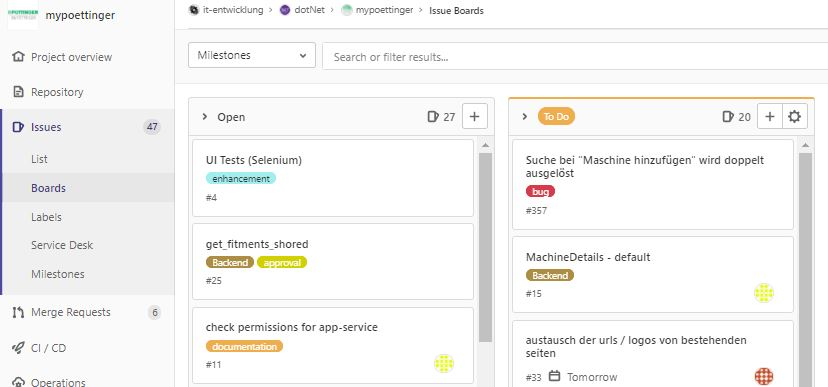
\includegraphics[width=0.8\textwidth]{./grafiken/GitLab_issue_Board.JPG}
	}
	\vskip0pt
	\caption{Das Issue-Board in GitLab (Bild wurde entnommen aus \cite{gitlabIssueBoard})}
\end{figure}


Im November 2019 haben wir begonnen uns mit der Firma Pöttinger Landtechnik GmbH und unserem Betreuer Herrn Rainer Sickinger abzusprechen.\\
Anschließend erfolgte die Erstellung des Pflichtenheftes, welches den Start der Projektarbeit darstellte. Finalisiert wurde das Pflichtenheft in Zusammenarbeit mit \ThPartnerPersonName \ in einem Meeting.\\
Im Juli 2020 begannen wir bei der Firma Pöttinger mit der Arbeit. Projektabschluss war im Februar 2021, wo der letzte Teil implementiert wurde.

\section{Meilensteine}
\begin{table}[H]
	\centering
{\rowcolors{2}{gray!20}{gray!10}
\begin{tabular}[h]{|l|p{8cm}|p{2.5cm}|p{2.5cm}|}
	\hline
	\# & Meilenstein & SOLL-Fertigstellung & IST-Fertigstellung \\
	\hline
	1 & Erstellung eines statischen Registrierungsformulars & Juli 2020 & Juli 2020 \\
	\hline
	2 & Aufbau einer dynamischen Internationalisierungsmöglichkeit & Juli 2020 & Juli 2020 \\	
	\hline
	3 & Erweiterung durch Komfortfeatures zur schnelleren/benutzerfreundlicheren Registrierung & Juli 2020 & Juli 2020 \\
	\hline
	4 & Schaffen von Login/Logout-Möglichkeiten & Juli 2020 & Juli 2020 \\	
	\hline
	5 & Entwicklung einer dynamisch generierten Registrierungsformulars & Juli 2020 & Juli 2020 \\	
	\hline
	6 & Gestaltung und Implementierung einer Profilseite zur Einsicht und Bearbeitung der Daten, sowie An-/Abmeldung zum Newsletter & Juli 2020 & Juli 2020 \\	
	\hline
	7 & Entwicklung des Maschinenparks & Juli 2020 & Juli 2020 \\	
	\hline
	8 & Einbinung der Module in die Startseite (Produktpalette / Maschinensuche / Konfigurator / PÖTSEM) & August 2020 & August 2020 \\	
	\hline
	9 & Implementierung der Startseite & August 2020 & August 2020 \\	
	\hline
	10 & CI/CD Pipeline & Jänner 2021 & Februar 2021 \\	
	\hline	
	11 & Diplomarbeit fertig verfasst & März 2021 & März 2021 \\
	\hline
\end{tabular}
}
\caption{Meilensteine}
\end{table}
Die definierten Meilensteine sind teils kleine Schritte, um den Grundstock für das weiterarbeiten zu ermöglichen. Da das Projektteam den gesamten Juli durcharbeitete, war es möglich, viele der Meilensteine in diesem einem Monat zu erreichen. 

%\section{Soll-Ist-Vergleich des Aufwandes}
%In der darunter stehenden Tabelle wird der geschätzte und der tatsächliche Aufwand in Stunden verglichen. 
	
	%%%%%%%%%%%%%%%%%%%%%%%%%%%%%%%%%%%%%%%%%
	%%%   VERWENDETE TECHNOLOGIEN   %%%%%%%%%
	%%%%%%%%%%%%%%%%%%%%%%%%%%%%%%%%%%%%%%%%%
	
	\chapter{Verwendete Technologien} \label{technologien}

\section{\LaTeX}
Diese Diplomarbeit wurde mit \LaTeX \space (\textit{{\bf{\textit{La}}}mport {\bf{\textit{\TeX}}}}) verfasst. Dieses Softwarepaket stellt eine Bibliothek von \TeX-Makros dar. \LaTeX \space ist plattformunabhängig und eine gute Möglichkeit gegenüber anderen Textverarbeitungsprogrammen. Dieses Softwarepaket funktioniert nach dem WYSIWYAF-Prinzip (\textit{{\bf{W}}hat {\bf{y}}ou {\bf{s}}ee {\bf{i}}s {\bf{w}}hat {\bf{y}}ou {\bf{a}}sked {\bf{f}}or}), das bedeutet es wird in normalen Textdateien mit Befehlen gearbeitet, die dann in verschiedene Formate (PDF, DVI, PostScript) kompiliert werden können. \autocite{wikiLatex}

\section{BibTeX}
BibTeX erstellt in \LaTeX-Dokumenten Literaturangaben und -Verzeichnisse. Dafür wird eine Literaturdatenbank, ein Textdokument mit der Endung .bib, erstellt, wo jedes Buch, Webseite oder Werk nach einer bestimmten Syntax hineingeschrieben wird. Zur Erstellung eines Verzeichnisses werden aus dem \LaTeX-Dokument alle Zitatverweise herausgesucht und mit der Literaturdatenbank zu einem Werk zugewiesen. Das Verzeichnis wird somit automatisch nach dem eingestellten Stil erstellt. \autocite{wikiBibtex}

\section{TeXstudio}
Die \LaTeX-Dokumente dieser Diplomarbeit wurden mit TeXstudio erstellt. Dieser Editor ist plattformunabhängig und er kompiliert und zeigt Dokumente an. Es besitzt eine Autocomplete-Funktion für \LaTeX-Befehle, Echtzeit-Syntaxkontrolle und -Rechtschreibüberprüfung. Weiteres besteht die Möglichkeit, dass Unicode-kodierte Dateien verarbeitet werden. \autocite{wikiTexstudio}


\section{Twilio} \label{sec:twilio}
Twilio wurde 2008 von Jeff Lawson, Evan Cooke und John Wolthuis in Amerika gegründet. Es betreibt eine Cloud-Kommunikationsplattform als Platform as a Service. Mit den von Twilio zur Verfügung gestellten Dienst, können Entwickler Programmierschnittstellen zum ausführen und empfangen von Anrufen, senden von SMS, verifizieren von Telefonnummern sowie für andere Kommunikationsfunktionen nutzen. In unseren Implementationen half Twilio bei der Verifizierung der von den Benutzer angegebenen Telefonnummern. \cite{twilioWebsite}

\section{Address Validator}
Der Address Validator wurde von Byteplant Software Solutions \& Services entwickelt. Dieses Unternehmen wurde 2003 in Deutschland gegründet. Neben dem Address Validator bieten sie auch einen Email Validator und einen Phone Validator an. Die Adressvalidierung hilft dabei, Informationen über die Zustellbarkeit einer Adresse zu sammeln, Korrekturvorschläge zu präsentieren, falls die Adresse nicht ganz gültig ist und eine einheitliche Adressformatierung nach den nationalen Standards anzubieten. Für eine Überprüfung benötigt man Straße, Stadt, Internationales Länderkürzel und den API-Key. Optional kann man noch mehr, wie beispielsweise Postleitzahl oder die Locale in der man das Ergebnis erhalten möchte, validieren. Als Antwort bekommt man eine Datei im JSON-Format. Aus dieser JSON-Datei ist es möglich, viele Informationen über die Adresse auszulesen. Falls die Adresse gültig ist, bekommt man im Feld Status ein VALID, bei ungültiger Adresse ein INVALID und falls die Überprüfung kein genaues Ergebnis herausgefunden hat, aber eine Adresse gefunden hat, die es sein könnte, ist der Status SUSPECT mit einen Adressvorschlag. Weiteres beinhaltet die Antwort alles von den einzelnen Adressfelder bis hin zu der formatierten Adresse des Landes und den Geografischen Koordinaten. \cite{addressValidator}

\section{Google Translator}
Die Schnittstelle für den Google Cloud Translator wurde von Google LLC entwickelt. Damit kann man schnell Texte in mehr als 100 Sprachen im eigenen Programm übersetzen lassen. Als Antwort der Übersetzung bekommt man den Titel, den Inhalt und die Abkürzung der Sprache. Nun kann man die Übersetzungen speichern und man braucht nur nach der Spachenabkürzung suchen.
\cite{googleTranslator}

\section{Auth0}
Auth0 wurde 2013 gegründet. Der Hauptsitz dieses Unternehmen liegt in Bellevue, Amerika. "Auth0 ist eine Identitätsmanagement Lösung, welche Sie in den Bereichen Authentifizierung, Registrierung und der Speicherung von Userdaten unterstützt. Über Auth0 kann ein Single sign-on von verschiedenen Plattformen und Applikationen (inklusive sozialer Kanäle wie Facebook, LinkedIn und Twitter) realisiert werden. Im Hintergrund können mehrere Datenquellen zum Login verwendet werden (Datenbank, ADFS, LDAP, etc.) Da Auth0 bereits mit einer Vielzahl an Connectors daher kommt, ist der Entwicklungsaufwand um ein Vielfaches kleiner als bei herkömmlichen Projekten." \autocite{auth0}

\section{Visual Studio Code}
Das Frontend dieser Diplomarbeit wurde in Visual Studio Code programmiert. Dieser Quelltexteditor erschien 2015 von Microsoft und arbeitet mit Quelldateien und Ordnern in Workspaces. Es bietet Versionsverwaltung, Autovervollständigung, Debugging und Syntaxhervorhebung. Es unterstützt Programmiersprachen wie Java, C++, C\#, JavaScript, TypeScript, Python und viele mehr. Für Visual Studio Code gibt es Plug-ins, die das programmieren sehr vereinfachen können. \autocite{wikiVisualStudioCode}

\begin{figure}[H]
	\centerline{
		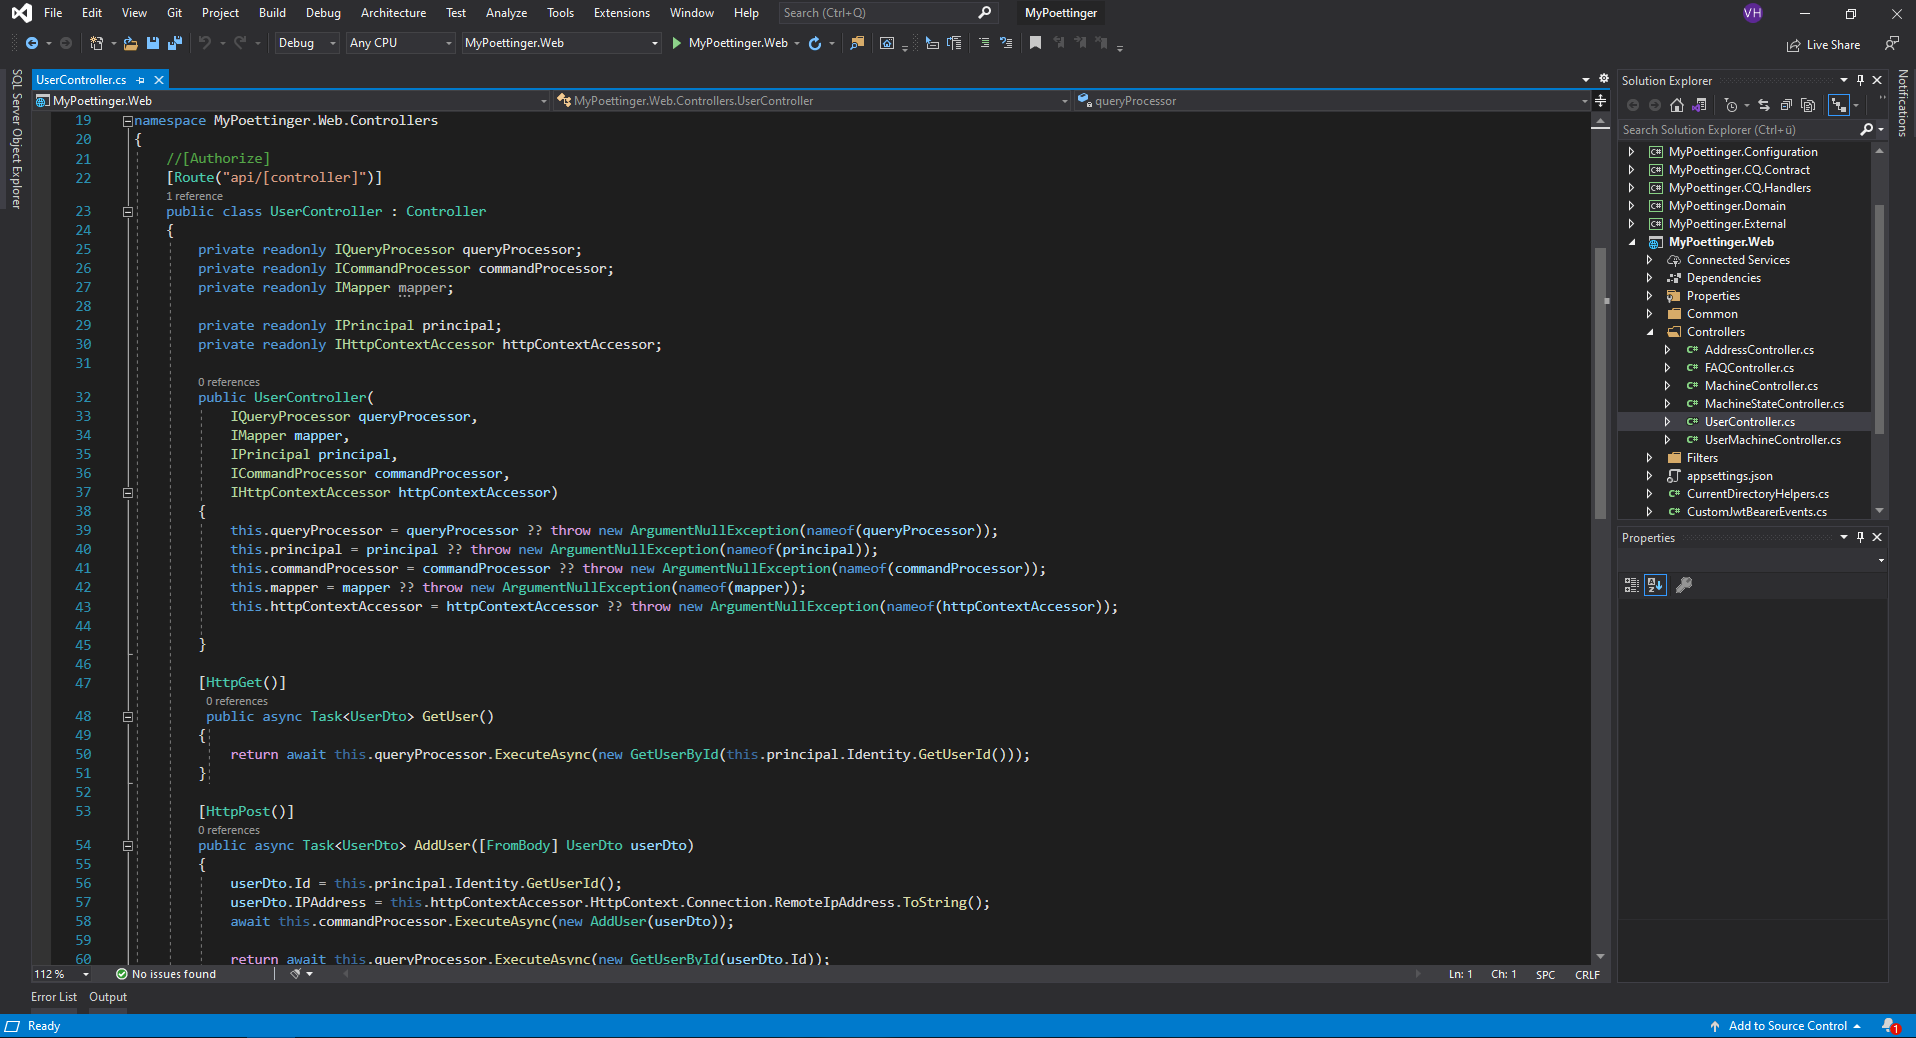
\includegraphics[width=0.8\textwidth]{./grafiken/visual_studio_startview.png}
	}
	\vskip0pt
	\caption{Screenshot vom Startbildschirm von Visual Studio Code} \label{fig:visualStudioCodeStartview}
\end{figure}

\section{Visual Studio 2019}
%Das Backend dieser Diplomarbeit wurde im Visual Studio programmiert. Die von Microsoft stammende Entwicklungsumgebung ist 1997 erschienen und arbeitet mit Projektdateien. Visual Studio bietet viele Funktionen wie IntelliSense, automatische Syntaxprüfung, Debugger mit Bearbeiten und Fortfahren und vieles mehr. Seit 2005 hat es einen integrierten Webserver. Es unterstützt einige Programmiersprachen, wie C\#, C++, C, Visual Basic .NET, TypeScript und viele mehr. \autocite{wikiVisualStudio}

Für das Backend der Diplomarbeit wurde Microsoft Visual Studio gewählt. Diese IDE (Integrated Development Environment) unterstützt den Programmierer durch eine ausgereifte Entwicklungsumgebung mit vielen Features.\\

Am nachfolgenden Screenshot sieht man den Startbildschirm von Microsoft Visual Studio 2019
\begin{figure}[h]
	\centerline{
	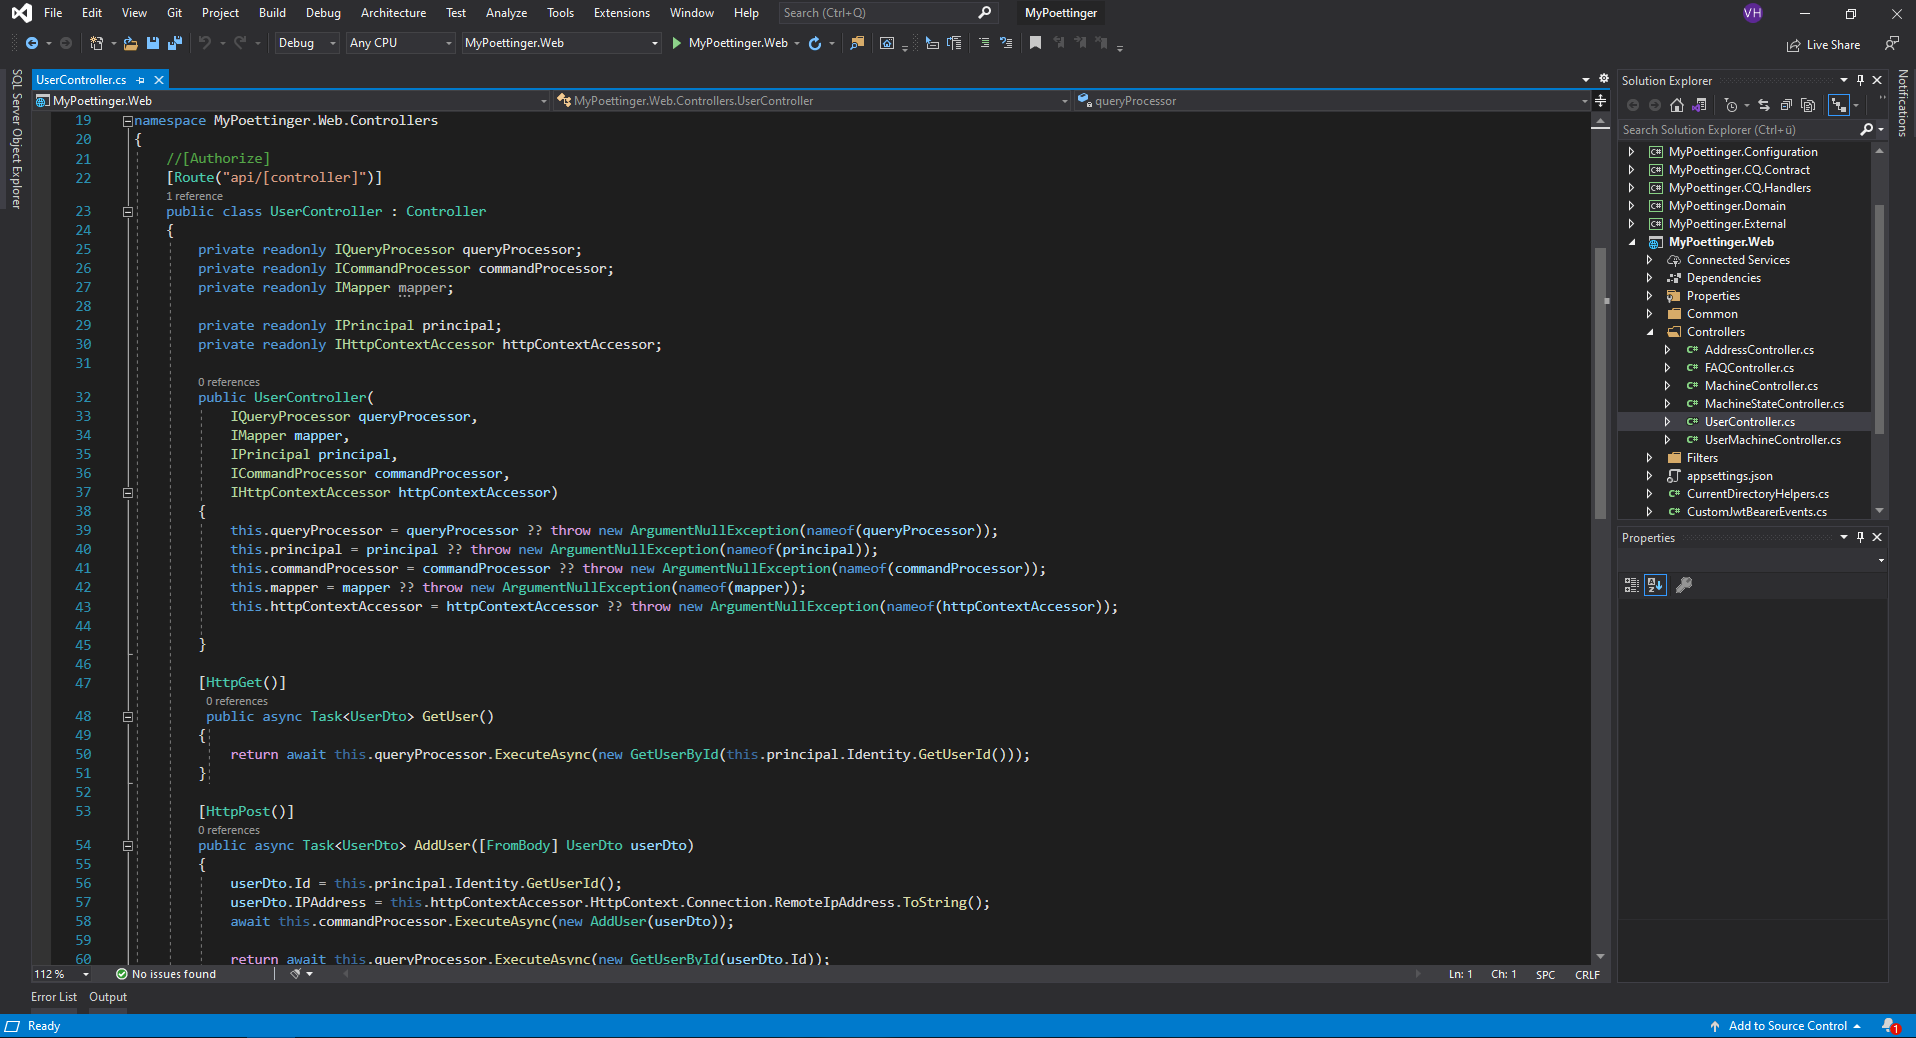
\includegraphics[width=0.8\textwidth]{./grafiken/visual_studio_startview.png}
	}
	\vskip0pt
	\caption{Screenshot vom Startbildschirm von Microsoft Visual Studio 2019} \label{fig:visualStudioStartview}
\end{figure}

Es gibt folgende Editionen von Microsoft Visual Studio 2019, wobei sie sich in den vorhandenen Funktionen unterscheiden:
\begin{itemize}
	\item Community Edition
	\item Professional Edition
	\item Test Professional Edition
	\item Enterprise Edition
\end{itemize}

Diese Diplomarbeit wurde mit der Community Edition erstellt, da diese Version alles zur Verfügung stellt, was gebraucht wurde. \autocite{wikiVisualStudio}

Micrsofot Visual Studio 2019 bietet viele unterstützende Features:
\begin{itemize}
	\item Online-Hilfe, die von der Cursorposition abhängig ist
	\item Ein- und Ausblenden von Codeblöcken
	\item Server-Explorer zum Zugriff auf Datenquellen
	\item Automatische Syntaxprüfung und IntelliSense
	\item Automatische Methoden- und Funktionsergänzung während der Quelltext-Eingabe
	\item Einbindung von Web Services
	\item ActiveX- und .NET-Bibliotheken
    \item Farbliche Kennung von Schlüsselwörtern
    \item Integrierter Debugger mit der Bearbeiten-und-Fortfahren-Funktion
	\item Windows-Nachrichtendienst
	\item WYSIWYG-Editoren zur Benutzeroberflächenentwicklung
\end{itemize}

\section{Postman}
Um die APIs (application programming interface) des Backendes der Diplomarbeit zu testen, wurde Postman verwendet. Postman bietet die Funktion, Http-Requests an jede beliebige URL mit jeder verfügbaren HTTP-Methode zu senden. Somit besteht die Möglichkeit, die programmierten Schnittstellen mit verschiedenen Daten schnell zu testen. Dieses Tool unterstützt SOAP, GraphQL und REST. Des weiteren ist Automated Testing möglich und es lassen sich Endpoints simulieren. Somit kann man das Verhalten der APIs sehr gut beobachten, was es einem Programmierer leichter macht Fehler zu finden. \autocite{postmanDocs} \\
Da das Backend dieser Diplomarbeit mit JWT (JSON Web Token) geschützt ist, ist es bei einem Postman-Request nötig diesen Token in den Header einzufügen, um die API zu testen.  \\
Am nachfolgenden Screenshot sieht man einen Request von Postman.
\begin{figure}[H]
	\centerline{
		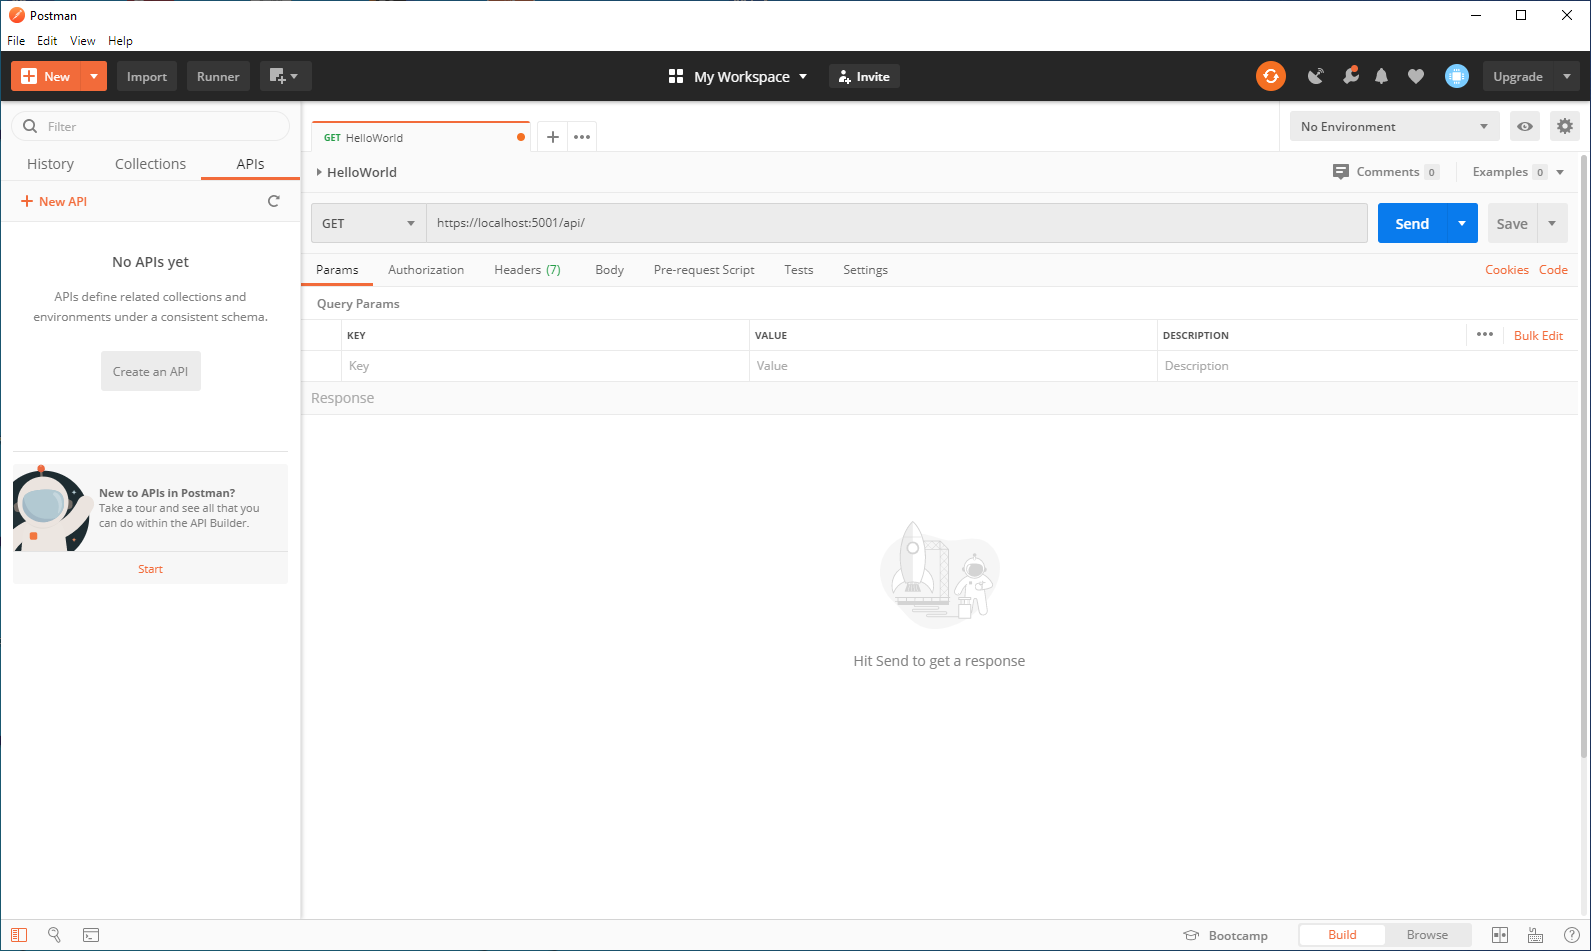
\includegraphics[width=0.8\textwidth]{./grafiken/postman.png}
	}
	\vskip0pt
	\caption{Screenshot von Postman} \label{fig:postman}
\end{figure}

\section{.NET Core 3.1 und C\#}
Für das Backend der Diplomarbeit wurde das Microsoft .NET Framework .NET Core 3.1 verwendet. Die Anwendungen wurden mit der objektorientierten Programmiersprache C\#  erstellt. \autocite{wikiDotnet}

\subsection{.NET Core 3.1}
.NET Core wurde 2015 als Abzweigung vom .NET Framework vorgestellt. Es wurde für eine bessere Modularität und eine leichtere Portierbarkeit auf Microsoft-fremde Plattformen entwickelt. 2016 wurde angekündigt, dass .NET Core mit mehr APIs ausgestatted wird, um die Kompatibilität zwischen verschiedenen .NET Frameworks zu verbessern. \autocite{wikiDotnet} \\
.NET Core 3.1 wurde am 03.12.2019 als Nachfolger von der Version 2.2 veröffentlicht. Dieses Framework unterstützt die Programmiersprachen C#, F#, C++/CLI und Visual Basic .NET. \autocite{wikiDotnetCore}

\subsection{C\#}
C\# wurde von Microsoft entwickelt und 2001 veröffentlicht. Diese plattformunabhängige, objektorientierte Programmiersprache basiert auf Konzepte von den Programmiersprachen Delphi, C, Haskell, C++ und Java.
C\# wird meist nicht gleich von den Compiler in die Maschinensprache, sondern in die Zwischensprache Common Intermediate Language (CIL) übersetzt. \autocite{wikiCSharp}

\begin{lstlisting}[caption={C\#-Syntaxbeispiel},captionpos=b, numbers=left, backgroundcolor=\color{black!10}, language={[Sharp]C}]
using System;
namespace HelloWorld
{
	public class Program
	{
		public static void Main(string[] args)
		{
			Console.WriteLine("Hello World!");
		}
	}
}
\end{lstlisting}

\section{JSON Web Token}
JSON Web Token(JWT) ist ein Access-Token, der auf JSON basiert. Durch JWT kann man verifizierbare Claims austauschen. Mit JWT sind Stateless Sessions möglich, da jede benötigte Information für eine Authentifikation mit dem Token übertragen werden kann. Ein JSON Web Token setzt sich aus dem Header, Payload und der Signatur zusammen. Bei einem Request mit einem Token schreibt man vor dem Token noch "Bearer". \autocite{wikiJWT}

Der Header ist ein JSON-Element. Darin ist gespeichert, welcher Token-Typ es ist und welche Verschlüsselungsmethode angewendet wird. Der Typ ist JWT und als Verschlüsselungsmethoden wird meist HMAC mit SHA-256 oder RSA mit SHA-256 verwendet. \autocite{wikiJWT} \\
\begin{lstlisting}[caption={JWT-Header Beispiel},captionpos=b, numbers=left, backgroundcolor=\color{black!10}, language=json]
{
	"alg": "HS256",
	"typ": "JWT"
}
\end{lstlisting}

Der Payload ist ebenfalls ein JSON-Element. In diesem JSON sind die Claims beschrieben. Es gibt einige reservierte Claims, die den Aussteller, das Subject oder das Ablaufdatum beschreiben, jedoch kann der Aussteller auch einen Private Claim definieren. \autocite{wikiJWT} \\
\begin{lstlisting}[caption={JWT-Payload Beispiel},captionpos=b, numbers=left, backgroundcolor=\color{black!10}, language=json]
	{
		"sub": "8135731594",
		"name": "Max Mustermann",
		"admin": true
	}
\end{lstlisting}

Durch JSON Web Signature(JWS) wird die Signature definiert. Die ist nach RFC 7515 genormt. Mit der im Header festgelegten Hashmethode wir der Header und der Payload Base64 kodierten und durch einem Punkt-getrenntem Format gehasht. Das Ergebnis ist die Signature. \autocite{wikiJWT}

Der JWT-Token setzt sich nun aus dem jeweils Base64-Url kodierten Header, Payload und Signature mit einem Punkt getrennt zusammen. \autocite{wikiJWT} \\
Der Nachfolgende Token setzt sich aus den zwei Beispielen zusammen:\\
\texttt{
eyJhbGciOiJIUzI1NiIsInR5cCI6IkpXVCJ9.eyJzdWIiOiI4MTM1NzMxNTk0IiwibmFtZSI6I\\k1heCBNdXN0ZXJtYW5uIiwiYWRtaW4iOnRydWV9.8NyZnCtWX\_QAlNhfl70zD2tHR\\9j1mtSl9Dwdfnnh60k
}
\section{Angular}
Das Frontend dieser Diplomarbeit wurde mit den Webapplikationsframework Angular geschrieben. Angular ist ein Open-Source-Software, basiert auf TypeScript und wird von einer Online-Community und Google LLC entwickelt.\\
Das Architekturkonzept von Angular ist eine Hierarchie von Komponenten. Durch Module wird Code schneller und Funktionalitäten können ausgelagert werden. TypeScript wird als Entwicklungssprache empfohlen, da diese Generics, statische Typisierung und klassenbasierte objektorientierte Programmierung ermöglicht. \autocite{wikiAngular}
Weiters bietet Angular:

\begin{itemize}
	\item Reaktive Programmierung mit RxJs
	\item Einfaches Routing
	\item Asynchrone Kompilierung von Templates
	\item Dynamisches Laden
	\item Dependency Injection
	\item Lazy- \& Eagerloading
\end{itemize}

\section{TypeScript}
TypeScript wurde von Microsoft entwickelt und 2012 veröffentlicht. Diese Programmiersprache basiert auf den ECMAScript6-Standard. Der TypeScript-Compiler kompliliert den Code in plain-JavaScript, deshalb ist jeder JavaScript-Code auch ein gültiger TypeScript-Code. Somit sind Bibliotheken wie jQuery oder AngularJS auch in TypeScript verwendbar. \autocite{wikiTypeScript} \\

TypeScript bietet viele unterstützende Features:

\begin{itemize}
	\item Klassen
	\item Module
	\item Arrow-Syntax für anonyme Funktionen
	\item Optionale Parameter und Standardparameter
	\item Namensräume
	\item Tupel
	\item Async/Await
	\item Generische Programmierung
	\item Aufzählungstyp
	\item Interfaces
	\item Type Erasure
	\item Typinferenz
	\item Methodensignatur
	\item Enums
\end{itemize}

\begin{lstlisting}[caption={TypeScript-Beispiel Function},captionpos=b, numbers=left, backgroundcolor=\color{black!10},language=JavaScript]
public add(a: number, b: number): number {
	return a + b;
}
\end{lstlisting}

\begin{lstlisting}[caption={TypeScript-Beispiel Klasse},captionpos=b, numbers=left, backgroundcolor=\color{black!10},language=JavaScript]
	class Person {
		private name: string;
		private age: number;
		private salary: number;
		
		constructor(name: string, age: number, salary: number) {
			this.name = name;
			this.age = age;
			this.salary = salary;
		}
		
		toString(): string {
			return `${this.name} (${this.age}): (${this.salary})`;
		}
	}
\end{lstlisting}
\begin{lstlisting}[caption={TypeScript-Beispiel Generische Programmierung},captionpos=b, numbers=left, backgroundcolor=\color{black!10},language=JavaScript]
	function doSomething<T>(arg: T): T {
		return arg;
	}
\end{lstlisting}

\section{Git Versionsverwaltung}
Git wurde 2005 veröffentlicht. Diese Software dient zur verteilten Versionsverwaltung von Dateien. Wichtige Bestandteile von Git sind die Erstellung neuer Entwicklungszweige, den sogenannten Branches und das Zusammenführen von zwei Zweigen. Da es keinen zentralen Server gibt, besitzt jeder Benutzer das gesamte Repository als Kopie lokal. Dadurch benötigt man für fast alle Aktionen keinen Internetzugriff. Mit den Hash-Wert eines Commites wird die History eines Projektes gespeichert. Durch diese Speicherung ist die History gesichert, da es nicht möglich ist, einen Commit zu verändern, der dann den selben Hash-Wert hat. \autocite{wikiGit}

\subsection{GitHub}
Für das Diplomarbeitsdokument wurde GitHub verwendet. GitHub wurde 2008 veröffentlicht und gehört seit 2018 zu Microsoft. Es dient zur Versionsverwaltung von Projekten. Diese Open-Source-Software ermöglicht ein leichtes Branching, Merging und Commiting für alle Entwickler. \autocite{wikiGitHub}

\begin{figure}[h]
	\centerline{
		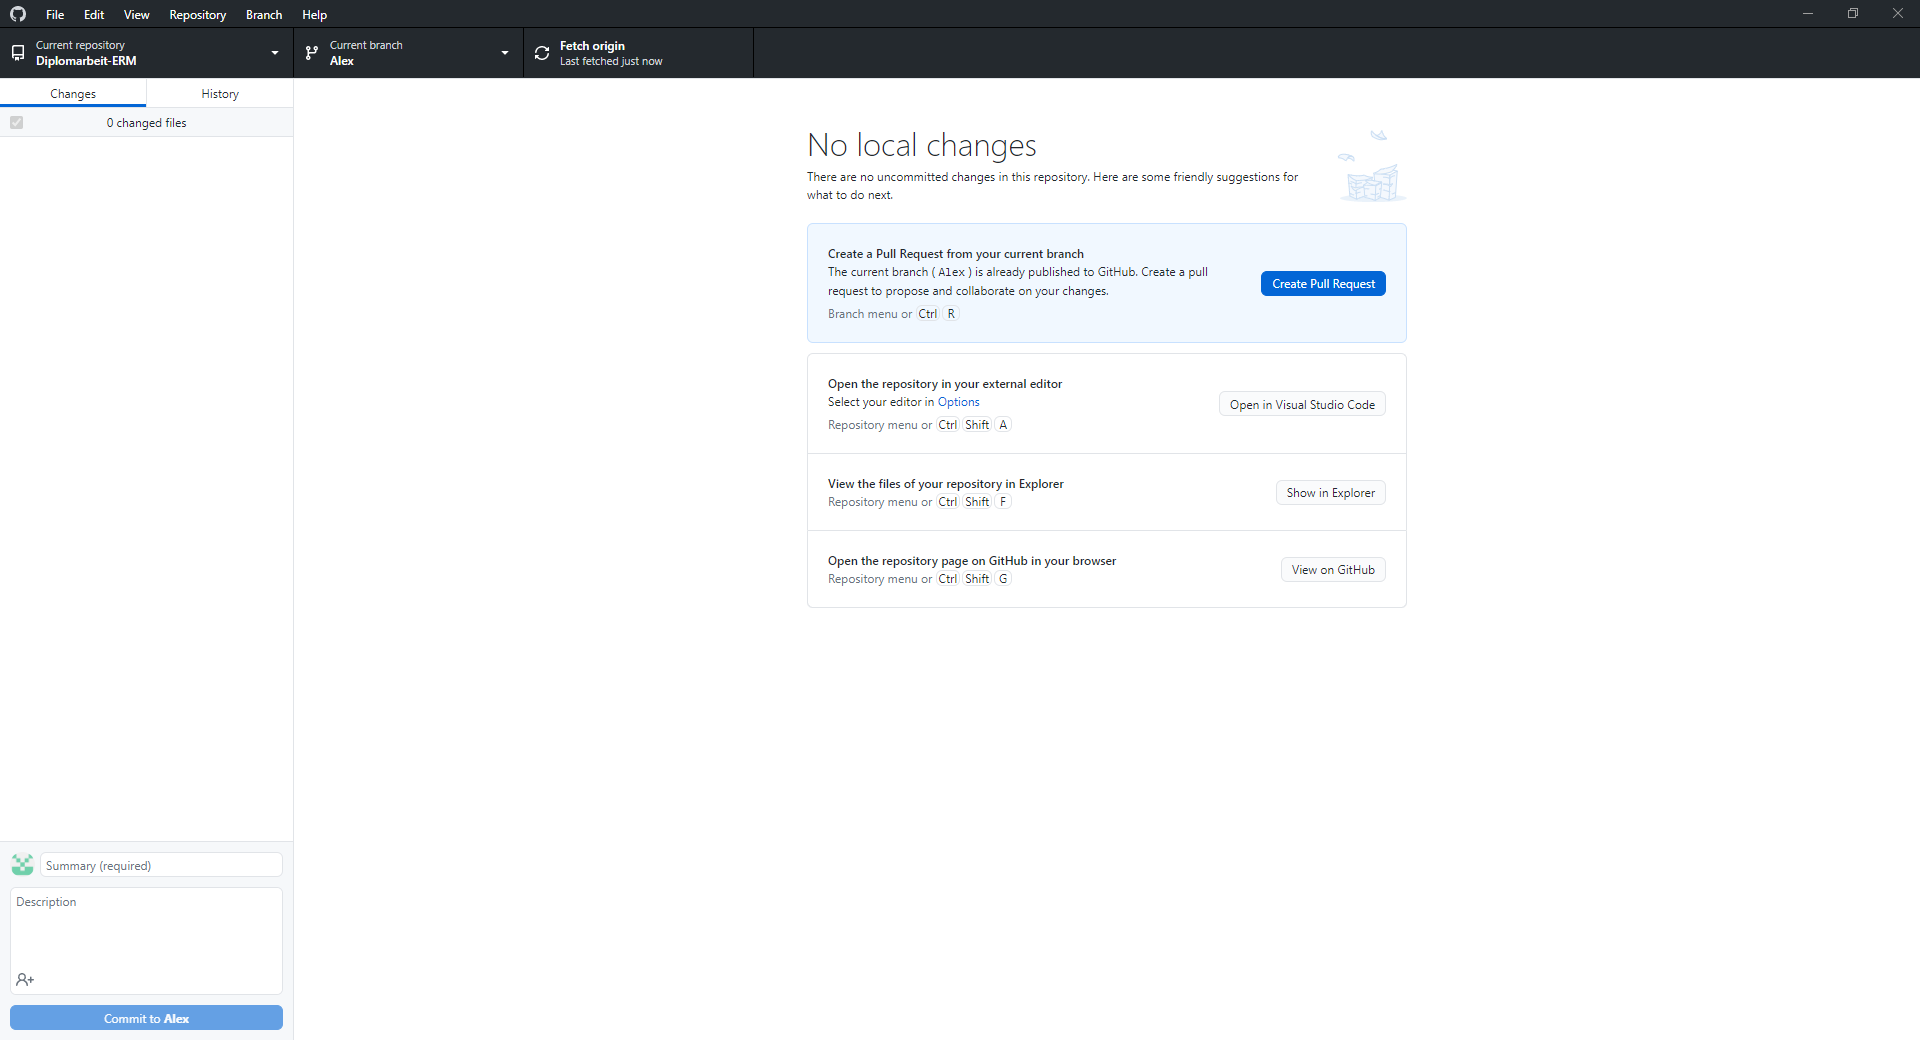
\includegraphics[width=0.8\textwidth]{./grafiken/github_screen.png}
	}
	\vskip0pt
	\caption{Screenshot von GitHub} \label{fig:github}
\end{figure}

\subsection{GitLab}
Für das Projekt der Diplomarbeit wurde GitLab verwendet. Die Versionsverwaltung basiert auf Git und ist eine Webanwendung. Weitere Features von GitLab ist ein Issue-Tracking-System mit einem Kanban-Board, ein Continuous Integration und Continuous Delivery System, eine Projekt-Wiki, eine Container-Registry und eine Multi-Cluster-Verwaltung. GitLab ist eine Open-Source-Software und wird als Software as a Service angeboten. \autocite{wikiGitLab}

\section{zxcvbn}
Um die Passwortstärke herauszufinden, wurde zxcvbn verwendet. Es erkennt und bewertet Passwörter durch Musterabgleich, Vergleich mit häufige Namen und Nachnamen, englische Wörter aus Wikipedia, Fernsehshows und Filme und Wiederholungen und Tastaturmuster. Als Antwort bekommt man Informationen, wie sicher das Passwort ist und ein Feedback mit einer Warnung und einem Tipp, wie man es noch sicherer machen könnte. \autocite{zxcvbn}
	
	%%%%%%%%%%%%%%%%%%%%%%%%%%%%%%%%%%%%%%%%%
	%%%   INTERNATIONALISIERUNG   %%%%%%%%%%%
	%%%%%%%%%%%%%%%%%%%%%%%%%%%%%%%%%%%%%%%%%
	
	\chapter{Internationalisierung}
In der Informatik bezeichnet man ein Programm als internationalisiert, wenn es mit dem unveränderten Quellcode in andere Sprachen und Kulturen übersetzt werden kann. Diese Bezeichnung wird oftmals als i18n abgekürzt. Die Zahl 18 steht für die Anzahl der Buchstaben, die sich zwischen dem ersten und den letzten Buchstaben im englischen Wort "internationalization" stehen. \autocite{wikii18n}
\section{Umsetzung}
Damit für eine Übersetzung der Quellcode nicht verändert werden muss, darf ein Text nicht hartkodiert sein. Für die verwendeten Texte sollen Variablen genutzt werden, die sich der gewünschten Sprache zur Laufzeit anpassen. Die Variablen werden in JSON-Dateien gespeichert und in den jeweiligen verfügbaren Sprachen übersetzt. Somit ergeben sich einige JSON-Dateien, die geladen werden können. Durch spezielle Plug-Ins ist es möglich, die neuen Variablen in einer Sprache selbst zu definieren und danach mit einem Klick in die gewünschten Sprachen übersetzen zu lassen. Dadurch füllen sich die weiteren JSON-Dateien.\autocite{wikii18n}\\
Im Bereich des RFs (Registrierungsformular) ist die Internationalisierung nicht nur für die Übersetzung integriert, sondern auch für den korrekten Aufbau und die Validierung der Felder. Dabei richtet sich die Reihenfolge der personenbezogenen Daten und der Adresseingabe und die Pflichtfelder nach dem Standard des ausgewählten Landes. Beispiele dafür sind Länder mit Provinzen oder welche, die keine Postleitzahlen besitzen. Solche Felder werden je nach Vorgabe angezeigt. Ein Beispiel für die veränderte Validierung ist die Länge der Postleitzahl, die sehr unterschiedlich sein kann.\autocite{wikii18n}
\section{Probleme}
Im Laufe der Zeit kann es sein, dass sich Texte ändern. Somit sind auch alle Translationen neu zu erstellen. Da nun der neu definierte Text möglicherweise länger oder kürzer ist, besteht die Gefahr, dass unerwünschte Lücken oder Textabschnitte entstehen. In verschiedenen Sprachen ist auch die Satzstellung unterschiedlich. Wird nun ein Satz mit einer eingesetzten Variable aus dem Programm angezeigt, ändert sich die Satzstellung. Ein Beispiel für Deutsch gegenüber Englisch wäre: "vor {variablen} Tagen" soll übersetzt "{Variable} days ago" heißen. Ein Lösungsansatz für dieses Problem ist die Verwendung von Platzhaltern.\autocite{wikii18n}
	
	%%%%%%%%%%%%%%%%%%%%%%%%%%%%%%%%%%%%%%%%%
	%%%   CQS   %%%%%%%%%%%%%%%%%%%%%%%%%%%%%
	%%%%%%%%%%%%%%%%%%%%%%%%%%%%%%%%%%%%%%%%%
	
	\chapter{Command-query Separation}
Das Prinzip der Command-query Separation (CQS) steht für die Trennung von Befehlen und Abfragen. In der klassischen Geschäftlogik-Schicht gibt es mehrere Schnittstellen, die verschiedenste Aufgaben abdecken. Da die Möglichkeit besteht, dass  mit der Zeit immer mehr Anforderungen an das System gestellt werden, werden die Schnittstellen und die darin befindenden Methoden immer mehr und möglicherweise auch die Cross-Cutting Concerns. Mit Cross-Cutting Concerns sind Anforderungen gemeint, die das ganze System betreffen, aber nicht von Anwendungsfall. Das können Transaktionen, Validierungen oder Rechteüberprüfungen sein. In dieser Diplomarbeit wurde bei jeden Aufruf geprüft, ob der Benutzer die berechtigten Rechte hat. Somit wäre ohne CQS in jeder Methode etwas zu ändern. \autocite{cqsSOLIDeArchitektur}\\
Um das umzusetzen, werden die zwei generische Schnittstellen benötigt, die man in Listing \ref{lst:cqsSchnittstellen} sieht. \texttt{IQuery} steht für Abfragen und \texttt{ICommand}, die für Aktionen steht.
\begin{lstlisting}[caption={CQS-Schnittstellen},captionpos=b, numbers=left, backgroundcolor=\color{black!10},language={[Sharp]C}, label={lst:cqsSchnittstellen}]
	public interface IQuery<TResult> { }
	public interface ICommand { }
\end{lstlisting}
Eine Methode aus dem Controller wird nun eine eigene Klasse. Als Eigenschaften dieser neuen Klasse werden die Methodenparameter verwendet. Ein Beispiel aus dieser Diplomarbeit kann man im Listing \ref{lst:getFaqbyid} sehen. Es implementiert dass im Listing \ref{lst:cqsSchnittstellen} vorhandene Interface \texttt{IQuery} mit dem Datentyp FAQDto.
\begin{lstlisting}[caption={CQS-Query Beispiel},captionpos=b, numbers=left, backgroundcolor=\color{black!10},language={[Sharp]C}, label={lst:getFaqbyid}]
	public class GetFAQById : IQuery<FAQDto>
	{
		public GetFAQById(Guid faqId)
		{
			this.FAQId = faqId;
		}
		public Guid FAQId { get;}
	}
\end{lstlisting}
Um die gewollte Logik auszuführen, werden zwei weitere generischen Schnittstellen benötigt. Wiederum gitb es eine für Abfragen und eine für Aktionen wie man im Listing \ref{lst:cqsHandler} sehen kann. Diese werden als Handler betitelt. \autocite{cqsSOLIDeArchitektur}
\begin{lstlisting}[caption={CQS-Handler},captionpos=b, numbers=left, backgroundcolor=\color{black!10},language={[Sharp]C}, label={lst:cqsHandler}]
	public interface IQueryHandler<TQuery, TResult>	where TQuery : IQuery<TResult>
	{
		Task<TResult> HandleAsync(TQuery query);
	}
	
	public interface ICommandHandler<TCommand> where TCommand : ICommand
	{
		Task HandleAsync(TCommand command);
	}
\end{lstlisting}
Den Handler für die im Listing \ref{lst:getFaqbyid} zu sehende Abfrage sieht man im Listing \ref{getFaqByIdHandler}.
\begin{lstlisting}[caption={CQS-Handler Beispiel},captionpos=b, numbers=left, backgroundcolor=\color{black!10},language={[Sharp]C}, label={getFaqByIdHandler}]
	internal class GetFAQByIdHandler : IQueryHandler<GetFAQById, FAQDto>
	{
		private readonly FAQRepositoryFactory faqRepositoryFactory;
		private readonly IMapper mapper;
		
		public GetFAQByIdHandler(
		FAQRepositoryFactory faqRepositoryFactory,
		IMapper mapper)
		{
			this.faqRepositoryFactory = faqRepositoryFactory ?? throw new ArgumentNullException(nameof(faqRepositoryFactory));
			this.mapper = mapper ?? throw new ArgumentNullException(nameof(mapper));
		}
		
		public async Task<FAQDto> HandleAsync(GetFAQById query)
		{
			using(var repository = this.faqRepositoryFactory())
			{
				var faq = (await repository.GetAsync(f => f.Id == query.FAQId))
				.SingleOrDefault()
				.ThrowIfNotFound(query.FAQId);
				faq.Fetches++;
				await repository.UpsertOneAsync(f => f.Id == faq.Id, faq);
				return this.mapper.Map<FAQDto>(faq);
			}
		}
	}
\end{lstlisting}
	
	%%%%%%%%%%%%%%%%%%%%%%%%%%%%%%%%%%%%%%%%%
	%%%   FAQ-Backend   %%%%%%%%%%%%%%%%%%%%%
	%%%%%%%%%%%%%%%%%%%%%%%%%%%%%%%%%%%%%%%%%

	\chapter{FAQ}
\section{Was ist FAQ}
FAQ steht für "Frequently Asked Questions". Es handelt sich dabei um eine Ansammlung von häufig gestellten Fragen, die auch für weitere Benutzer interessant sein könnten. Somit findet man auf einer Webseite im Bereich FAQ eine Auflistung dieser Ansammlung der wiederkehrenden Benutzerfragen.
\section{FAQ-Backend}
Eine der Aufgaben war, ein funktionierendes Backend für einen zukünftigen FAQ-Bereich zu programmieren. Im Allgemeinen, ging es darum, wenn eine Frage gestellt wird, wird diese bearbeitet. Wenn die Person, die diese Frage bearbeitet und beantwortet, empfindet, diese Frage könnte auch noch für weitere Benutzer von Interesse sein und diese Person hat auch die benötigten Rechte dafür, kann sie aus dieser Frage ein FAQ erstellen.\\
Dafür wurde zuerst eine Tabelle in der Datenbank definiert. Ein FAQ besteht in der Datenbank aus einer ID, einem Sprachenkürzel, dem Titel, den Inhalt der Frage, einem Zähler, der die Abfragen mitzählt und einer Liste mit den vorhandenen Übersetzungen für diese Frage. Die Berechtigung ist mit einem Claim in dem JWT gespeichert. Wenn nun der Befehl um eine FAQ zu erstellen aufgerufen wird, wird zuerst überprüft, ob die benötigte Berechtigung vorhanden ist. Falls vorhanden, wird die FAQ erstellt und automatisch mit Google Cloud Translate übersetzt und gespeichert. In diesen folgenden Sprachen ist die FAQ danach übersetzt:
\begin{multicols}{2}
	\begin{itemize}
		\item Deutsch
		\item Englisch
		\item Französisch
		\item Niederländisch
		\item Dänisch
		\item Spanisch
		\item Italienisch
		\item Ungarisch
		\item Polnisch
		\item Slowakisch
		\item Finnisch
		\item Schwedisch
		\item Tschechisch
		\item Russisch
		\item Ukrainisch
	\end{itemize}
\end{multicols}
	
	%%%%%%%%%%%%%%%%%%%%%%%%%%%%%%%%%%%%%%%%%
	%%%   REGISTRIERUNGSFORMULAR   %%%%%%%%%%
	%%%%%%%%%%%%%%%%%%%%%%%%%%%%%%%%%%%%%%%%%
	
	\chapter{Das Registrierungsformular}

Der wohl komplizierteste Teil dieser Diplomarbeit ist der Aufbau und die korrekte Validierung des Registrierungsformulars. Das Ziel ist den Benutzern eine möglichst einfache und schnelle Registrierung, unter Berücksichtigung des derzeitigen Standorts und der dazugehörigen Benutzergruppe, anzubieten. Dafür wurde ein Algorithmus entwickelt, welcher bei der \texttt{ngAfterViewInit} Lifecycle-Hook-Methode im \texttt{UserprofileComponent} seinen Start nimmt.

\section{Der Algorithmus hinter dem dynamischen Aufbau}

\begin{figure}[H]
	\centerline{
		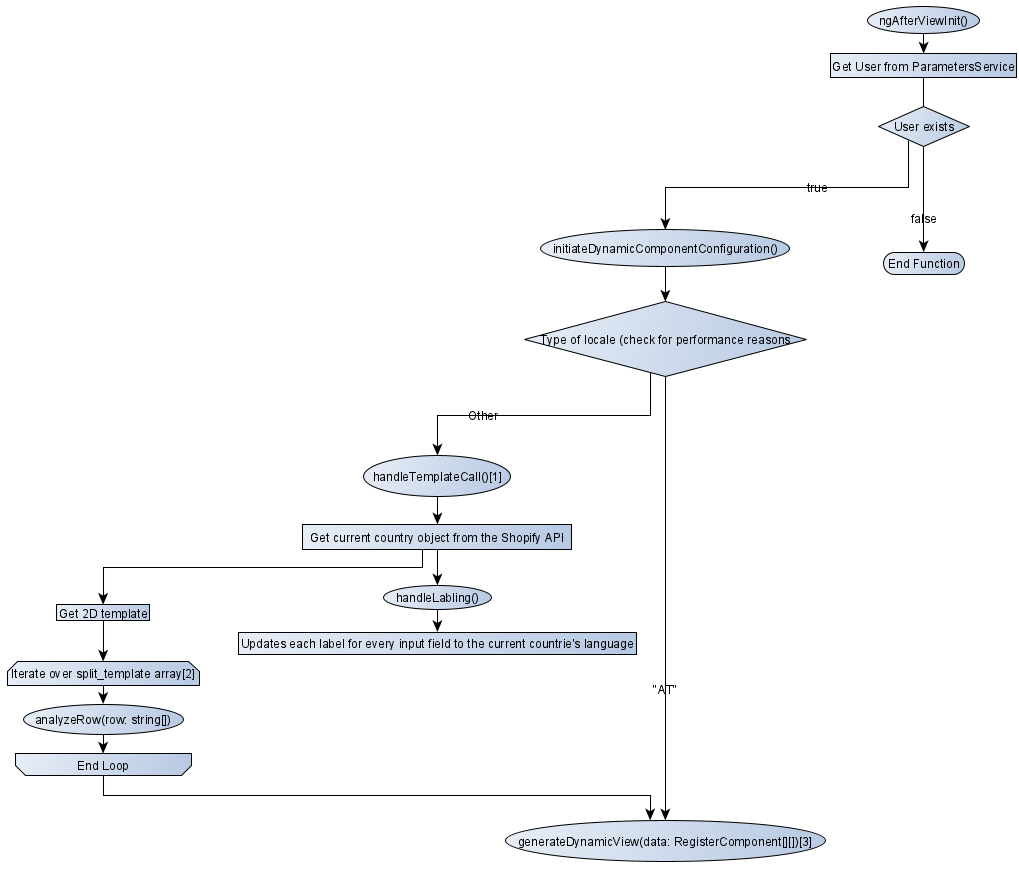
\includegraphics[width=1\textwidth, frame]{./grafiken/RF_Flussdiagramm.png}
	}
	\vskip0pt
	\caption{Flussdiagramm des Algorithmus}
	\label{fig:fc}
\end{figure}

Wenn das User-Objekt, welches von der Backend API abgefragt und erfolgreich als globale Objekt variable gespeichert wurde, wird die \texttt{initiateDynamicComponentConfigu\\ration()}-Methode aufgerufen. Aus Performance-Gründen basiert die nächste Überprüfung auf den Wert der aktuellen Lokale. Gleicht dieser den Wert "AT", so wird ein vorgefertigtes Template für ein österreichisches RF, dargestellt im Listing~\ref{lst:template_form_aut}, für die Weiterverwendung benützt. Da davon ausgegangen wird, dass sich vor allem in der Anfangsphase nach der Veröffentlichung hauptsächlich österreichische Kunden ein Konto erstellen, spart dieser Weg enorm viel Zeit, da sofort mit der Erstellung des RF begonnen werden kann.

\begin{lstlisting}[caption={Vordefiniertes Template für das RF},captionpos=b, language=JavaScript,label={lst:template_form_aut}]
export const AUSTRIAN_PRIVATE_PERSON_FORM_Template = [
	[{ type: GenderComponent }],
	[
		{ type: FirstnameComponent, options: { label: "Vorname" } },
		{ type: LastnameComponent, options: { label: "Nachname" } },
	],
	[{ type: StreetComponent, options: { label: "Straße und Hausnummer" } }],
	[
		{ type: CityComponent, options: { label: "Stadt" } },
		{ type: PostalcodeComponent, options: { label: "Postleitzahl" } },
	],
	[
	{
		type: PhoneComponent,
		options: { label: "Telefonnummer", phonePrefix: 43 },
	},
	{ type: DateofbirthComponent },
	],
];
\end{lstlisting}

Anderenfalls wird als nächster Schritt die \texttt{handleTemplateCall()}-Methode aufgerufen, markiert im Flussdiagramm~\ref{fig:fc} mit [1], welche, basierend auf den Wert der aktuellen Lokale, auf die Shopify API zugreift, um ein \texttt{Country}-Objekt abzurufen. Wurde diese Operation beendet folgt ein Update auf die Labels für den Wrapper der Objekte für das RF. Nach dem das Template geladen wurde, wird über jedes einzelne Element iteriert, markiert im Flussdiagramm~\ref{fig:fc} mit [2], um daraus eine oder mehrere Zeilen zu generieren. Anschließend werden diese in ein 2D Array gespeichert, welches dann der \texttt{generateDynamicView()}-Methode zu Generierung des RF übergeben wird. 

\begin{lstlisting}[caption={Erstellung des 2D Arrays für den Aufbau des RF},captionpos=b, language=JavaScript,label={lst:analyzeRow}]
private analyzeRow(row: string[]): RegisterComponent[][] {
	let addGenderC = false;
	let result: RegisterComponent[][] = [];
	let componentRow: RegisterComponent[] = [];
	
	for (let i = 0; i < row.length; i++) {
		let rowEl = row[i];
		
		if (!addGenderC) {
			if (rowEl.includes("firstName") || rowEl.includes("lastName")) {
				let genderComponent: RegisterComponent[] = [
				{ type: GenderComponent },
				];
				result.push(genderComponent);
				addGenderC = true;
			}
		}
		
		if (rowEl.includes("company") && this.user.isPrivatePerson) {
			break;
		}
		
		for (const x of this.valueMap.keys()) {
			if (rowEl.includes(x)) {
				let compEl: RegisterComponent = {
					type: this.valueMap.get(x),
				};
				
				if (
				compEl.type.prototype ===
				ZoneComponent.prototype
				) {
					compEl.options.zones = this.countryFromService.zones.map(
					(x) => x.name
					);
					this.user.zone = compEl.options.zones[0];
				}
				
				if (
				compEl.type.prototype ===
				PhoneComponent.prototype
				) {
					compEl.options.phonePrefix = this.countryFromService.phoneNumberPrefix;
				}
				
				if (this.labels.get(x)) {
					compEl.options.label = this.labels.get(x);
				}
				
				componentRow.push(compEl);
				if (rowEl.includes("phone")) {
					let dateofbirthComponent: RegisterComponent = {
						type: DateofbirthComponent,
					};
					componentRow.push(dateofbirthComponent);
				}
				break;
			}
		}
	}
	result.push(componentRow);
	return result;
}
\end{lstlisting}

Die im Listing~\ref{lst:analyzeRow} beschriebene \texttt{analyzeRow()}-Methode nimmt ein Array von Zeichenfolgen als Parameter und gibt ein 2D-Array von \texttt{RegisterComponent}-Wrapper-Objekten zurück. Obwohl nur eine Reihe aus dem Template, also z. B. \texttt{[\{firstName\} \{lastname\}]}, überprüft wird, kann es wie in diesem Fall sein, dass ein Input zusätzlich darüber erzeugt werden muss. So wird in Zeile 9 überprüft, ob der \texttt{GenderComponent} schon hinzugefügt wurde. Trifft das und die Überprüfung, ob in diesem Durchgang der \texttt{FirstnameComponent} und der \texttt{LastnameComponent} erzeugt werden, wird der \texttt{GenderComponent} als erster eingefügt. Dieser ist für die Auswahl der Anrede zuständig. Der selbe Mechanismus kann auch in Zeile 51 gefunden werden, wo es nötig ist, den \texttt{DateofbirthComponent}, welcher für die Eingabe des Geburtstages verantwortlich ist, neben den \texttt{PhoneComponent} zu generieren.

Anschließend wird in Zeile 19 sicher gestellt, dass eine Privatperson keine Auswahl einer Firma präsentiert wird.

Um nun tatsächlich aus dem Template Objekte zu erzeugen, wird ab Zeile 23 über Schlüssel einer Map, beschrieben im Listing~\ref{lst:valueMap}, welche den String eines Templates als \texttt{key} und den korrespondierenden Objekten als \texttt{value} hat, iteriert. 

\begin{lstlisting}[caption={Vordefiniertes Template für das RF},captionpos=b, language=JavaScript,label={lst:valueMap}]
export class ValueMapper {
	static COMPONENT_VALUE_MAP: Map<string, Type<any>> = new Map();
	
	static COMPONENT_VALUE_MAPPER(){
		this.COMPONENT_VALUE_MAP.set('firstname', FirstnameComponent);
		this.COMPONENT_VALUE_MAP.set('lastname', LastnameComponent);
		this.COMPONENT_VALUE_MAP.set('company', BusinessNameComponent);
		this.COMPONENT_VALUE_MAP.set('address1', StreetComponent);
		this.COMPONENT_VALUE_MAP.set('zip', PostalcodeComponent);
		this.COMPONENT_VALUE_MAP.set('city', CityComponent);
		this.COMPONENT_VALUE_MAP.set('phone', PhoneComponent);
		this.COMPONENT_VALUE_MAP.set('dateOfBirth', DateofbirthComponent);
		this.COMPONENT_VALUE_MAP.set('gender', GenderComponent);
		this.COMPONENT_VALUE_MAP.set('zone', ZoneComponent);
		this.COMPONENT_VALUE_MAP.set('province', ZoneComponent);
		this.COMPONENT_VALUE_MAP.set('state', ZoneComponent);
		return ValueMapper.COMPONENT_VALUE_MAP;
	}
}
\end{lstlisting}


\section{Die Validierungsmethodik}

\section{Die Komfortfunktionen}

\begin{figure}[H]
	\centerline{
		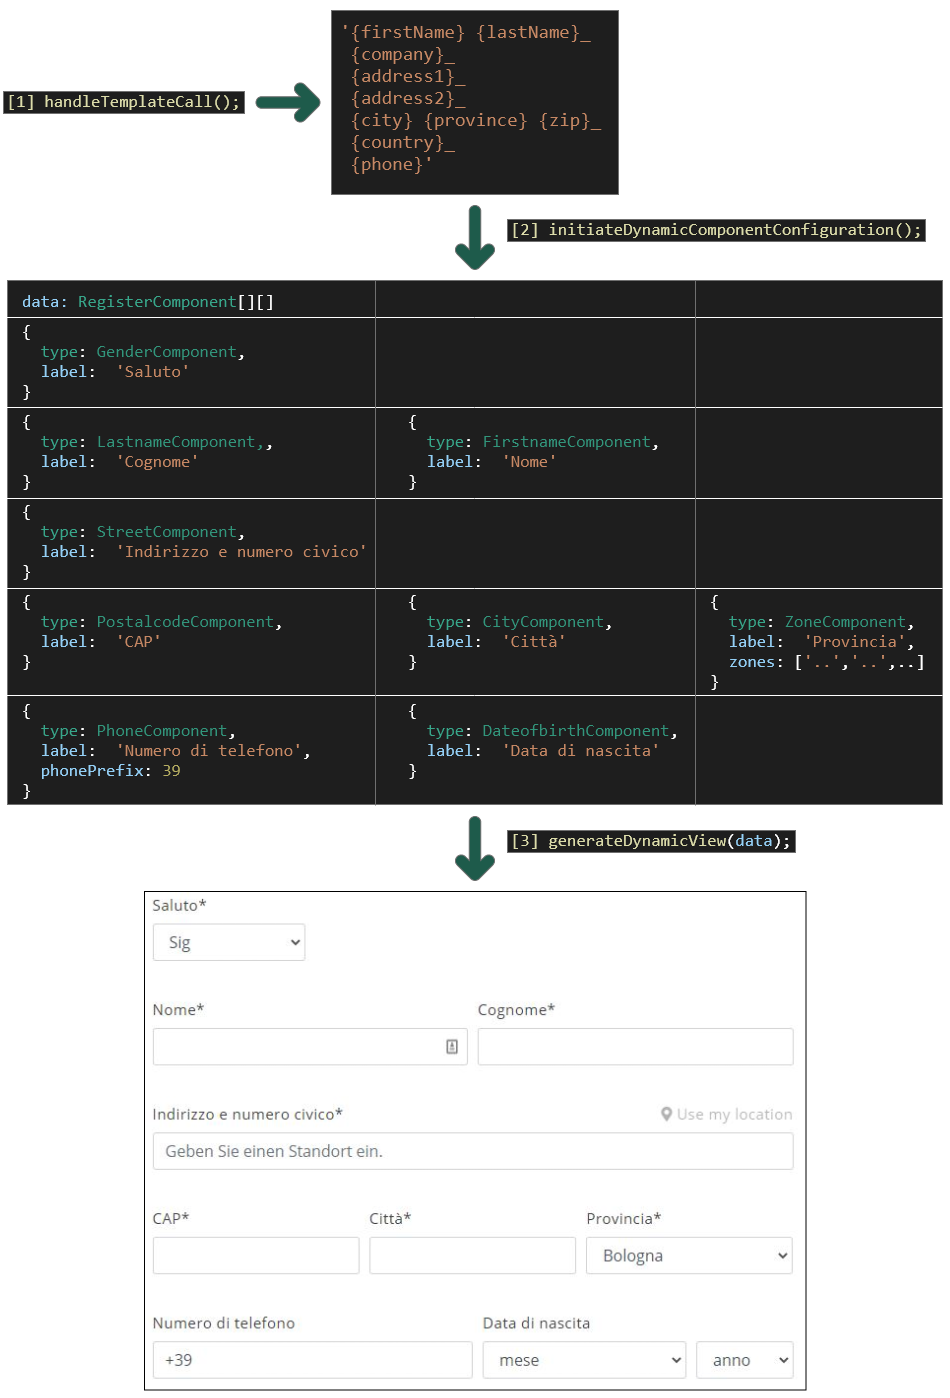
\includegraphics[width=1\textwidth, frame]{./grafiken/RF_Datenvisualisierung.png}
	}
	\vskip0pt
	\caption{Visualisierter Datenfluss vom Template bis zum fertigen RF}
\end{figure}


	
	%%%%%%%%%%%%%%%%%%%%%%%%%%%%%%%%%%%%%%%%%
	%%%   CI / CD   %%%%%%%%%%%%%%%%%%%%%%%%%
	%%%%%%%%%%%%%%%%%%%%%%%%%%%%%%%%%%%%%%%%%
	
	\chapter{CI / CD}
\section{Was ist CI/CD}

Es handelt sich hier um eine Methode, bei der den Kunden regelmäßig Apps bereitgestellt und alle Phasen der Anwendungsentwicklung automatisiert werden. Die Hauptkonzepte von CI/CD sind Continuous Integration, Continuous Delivery und Continuous Deployment. CI/CD löst die Probleme, welche die Integration von neuem Code für DevOps-Teams verursachen kann.\cite{whatIsCICD}

Insbesondere sorgt CI/CD für eine kontinuierliche Automatisierung und Überwachung über den gesamten App-Lifecycle hinweg, von der Integrations- und Test- bis hin zur Bereitstellungs- und Implementierungsphase. Diese zusammenhängenden Praktiken werden oft als „CI/CD-Pipeline“ bezeichnet, und sie werden durch eine agile Zusammenarbeit der DevOps-Teams unterstützt.\autocite{whatIsCICD}

Die Abkürzung CI/CD hat unterschiedliche Bedeutungen. „CI“ bedeutet Continuous Integration, also der Automatisierungsprozess für Entwickler. Bei einer erfolgreichen CI werden regelmäßig neue Codeänderungen für Apps entwickelt, geprüft und in einem gemeinsamen Repository zusammengeführt. Damit soll der Konflikt verhindert werden, den zu viele Branches einer App verursachen können, wenn sie zeitgleich entwickelt werden.\autocite{whatIsCICD}

„CD“ bedeutet Continuous Delivery bzw. Continuous Deployment. Das sind verwandte Konzepte, die zuweilen synonym verwendet werden. Obwohl es bei beiden Konzepten um die Automatisierung weiterer Phasen der Pipeline geht, werden die Begriffe manchmal unterschiedlich verwendet, um das Ausmaß der Automatisierung zu verdeutlichen.\autocite{whatIsCICD}

Continuous Delivery bedeutet üblicherweise, dass App-Änderungen eines Entwicklers automatisch auf Bugs getestet und in ein Repository (wie GitHub oder eine Container-Registry) hochgeladen werden, von wo aus sie vom Operations-Team in einer Live-Produktivumgebung bereitgestellt werden können. Dieser Vorgang ist die Antwort auf Transparenz- und Kommunikationsprobleme zwischen Dev- und Business-Teams. Damit soll sichergestellt werden, dass neuer Code mit minimalem Aufwand implementiert werden kann.\autocite{whatIsCICD}

Continuous Deployment (das andere „CD“) kann sich auf die automatische Freigabe von Entwickleränderungen vom Repository zur Produktivphase beziehen, wo sie direkt vom Kunden genutzt werden können. Dieser Vorgang soll der Überlastung von Operations-Teams bei manuellen Prozessen entgegenwirken, die die Anwendungsbereitstellung verlangsamen. Continuous Development baut die Vorteile der Continuous Delivery aus, indem auch noch die nächste Phase der Pipeline automatisiert wird.\autocite{whatIsCICD}

\begin{figure}[H]
	\centerline{
		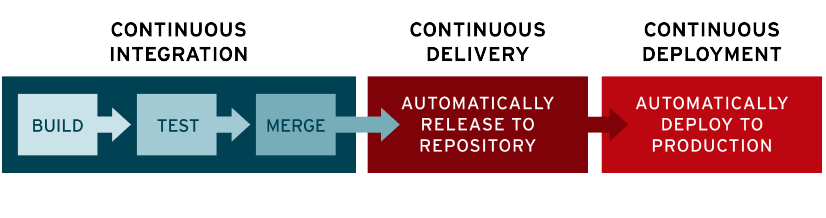
\includegraphics[width=1\textwidth, frame]{./grafiken/ci-cd-flow-redhatsource.png}
	}
	\vskip0pt
	\caption{CI/CD Workflow (Bild wurde entnommen aus \cite{whatIsCICD})}
\end{figure}


Manchmal sind mit CI/CD lediglich die zusammenhängenden Praktiken der Continuous Integration und der Continuous Delivery, manchmal aber auch alle drei Konzepte der Continuous Integration, Continuous Delivery und Continuous Deployment gemeint. Noch komplizierter wird das Ganze dadurch, dass mit Continuous Delivery zuweilen auch die Prozesse des Continuous Deployment mitgemeint sind.\autocite{whatIsCICD}

Letztendlich bringen uns diese Details jedoch nicht weiter. Man sollte CI/CD einfach als Prozess ansehen, der nicht selten als Pipeline visualisiert wird und der ein hohes Maß an kontinuierlicher Automatisierung und Überwachung bei der Anwendungsentwicklung umfasst. Je nach Fall hängt die Auslegung des Begriffs vom Grad der Automatisierung der CI/CD-Pipeline ab. Viele Unternehmen arbeiten zunächst mit CI und setzen den Prozess später mit der automatischen Bereitstellung und Implementierung fort, z. B. bei cloudnative Apps.\autocite{whatIsCICD}

\section{Continuous Integration}

Bei der modernen Anwendungsentwicklung arbeiten mehrere Entwickler an unterschiedlichen Features der gleichen App. Die gleichzeitige Zusammenführung aller Quellcode-Branches an einem Tag (auch bekannt als „Merge Day“) kann einen hohen Arbeits- und Zeitaufwand bedeuten. Der Grund dafür ist, dass Anwendungsänderungen von getrennt arbeitenden Entwicklern miteinander in Konflikt treten können, wenn sie zeitgleich durchgeführt werden. Dieses Problem kann sich verschlimmern, wenn jeder Entwickler seine eigene lokale Integrated Development Environment (IDE) definiert, statt im Team eine gemeinsame cloudbasierte IDE zu erstellen.\autocite{whatIsCICD}

Mithilfe der Continuous Integration (CI) können Entwickler ihre Codeänderungen in einem gemeinsamen „Branch“ oder „Trunk“ der Anwendung viel häufiger zusammenführen, manchmal sogar täglich. Sobald die Änderungen eines Entwicklers zusammengeführt werden, werden sie in automatischen App-Builds und unterschiedlichen Stufen von Automatisierungsprüfungen (normalerweise Einheits- und Integrationstests) validiert. So wird sichergestellt, dass die Funktionsfähigkeit nicht beeinträchtigt wurde. Dabei müssen alle Klassen und Funktionen bis hin zu den verschiedenen Modulen der App getestet werden. Wenn die automatische Prüfung Konflikte zwischen aktuellem und neuem Code erkennt, lassen sich diese mithilfe von CI schneller und häufiger beheben.\autocite{whatIsCICD}

\section{Continuous Delivery}

Nach der Automatisierung von Builds und Einheits- und Integrationstests bei der CI wird bei der Continuous Delivery auch die Freigabe des validierten Codes an ein Repository automatisch durchgeführt. Um also einen effizienten Continuous Delivery-Prozess zu gewährleisten, muss die CI bereits in Ihre Entwicklungs-Pipeline integriert sein. Ziel der Continuous Delivery ist eine Codebasis, die jederzeit in einer Produktivumgebung bereitgestellt werden kann.\autocite{whatIsCICD}

Bei der Continuous Delivery umfasst jede Phase − von der Zusammenführung der Codeänderungen bis zur Bereitstellung produktionsreifer Builds − automatisierte Tests und Code-Freigaben. Am Ende dieses Prozesses kann das Operations-Team eine App schnell und einfach in der Produktivphase bereitstellen.\autocite{whatIsCICD}

\section{Continuous Deployment}

Die abschließende Phase der CI/CD-Pipeline ist das Continuous Deployment. Als Erweiterung der Continuous Delivery, bei der produktionsreife Builds automatisch an ein Code-Repository freigegeben werden, wird beim Continuous Deployment auch die Freigabe einer App in die Produktivphase automatisiert. Da der Produktivphase in der Pipeline kein manuelles Gate vorgeschaltet ist, müssen beim Continuous Deployment die automatisierten Tests immer sehr gut durchdacht sein.\autocite{whatIsCICD}

In der Praxis bedeutet Continuous Deployment, dass App-Änderungen eines Entwicklers binnen weniger Minuten nach ihrer Erstellung live gehen können (vorausgesetzt, sie bestehen den automatischen Test). Dies erleichtert eine kontinuierliche Integration von User Feedback ungemein. All diese zusammenhängenden CI/CD-Praktiken machen eine Anwendungsimplementierung weniger riskant, weil Änderungen in Teilen und nicht auf einmal freigegeben werden. Die Vorabinvestitionen sind allerdings beträchtlich, da automatische Tests für die diversen Prüf- und Release-Phasen in der CI/CD-Pipeline geschrieben werden müssen.\autocite{whatIsCICD}

\section{GitLab Pipeline}

Pipelines sind top-level Komponenten der Continuous Integration, Delivery und Deployment. Pipelines umfassen:\autocite{gitlabPipelines}

\begin{itemize}
	\item Jobs, welche definieren \textit{was} auszuführen ist. Zum Beispiel gibt es Jobs, welche den Code kompilieren, Pakete installieren und testen.
	\item Stages, welche definieren \textit{wann} Jobs auszuführen sind. Beispielsweise ist die Kompile-Stage üblicherweise vor der Test-Stage.
\end{itemize}

Jobs werden von Runner ausgeführt. Mehrere Jobs in der selben Stage werden parallel ausgeführt, wenn genügend simultane Runner bereitstehen.
Wenn \textit{alle} Jobs in einer Stage erfolgreich ausgeführt wurden, geht die Pipeline zur nächsten Stage über.
Wenn \textit{irgendein} Job in einer Stage fehlschlägt, wird die nächste Stage (normalerweise) nicht ausgeführt und die Pipeline endet vorzeitig.\autocite{gitlabPipelines}

Im Allgemeinen werden Pipelines in der Regel automatisch  nach dem Hochladen eines Commits ausgeführt und erfordern nach ihrer Erstellung keinen weiteren manuellen Eingriff.
Eine typische Pipeline kann aus vier Phasen bestehen, die in der folgenden Reihenfolge ausgeführt werden:\autocite{gitlabPipelines}

\begin{itemize}
	\item Eine \texttt{Build-Stage}, mit einem \texttt{Compile-Job}.
	\item Eine \texttt{Test-Stage}, welche mehrere \texttt{Test-Jobs} beinhalten kann.
	\item Eine \texttt{Staging-Stage}, mit einem \texttt{Deploy-to-Stage-Job}.
	\item Eine \texttt{Production-Stage}, mit einem \texttt{Deploy-to-Production-Job}.
\end{itemize}

\section{GitLab Runner} \label{sec:lblGitLabRunner}
\subsection{Registrierung}

GitLab Runner ist eine Anwendung, die mit GitLab CI/CD arbeitet, um Aufträge in einer Pipeline auszuführen.
Man kann die GitLab Runner-Anwendung auf der Infrastruktur installieren, besitzen oder verwalten. In diesem Fall sollte man GitLab Runner auf einem Rechner installieren, der von dem Rechner getrennt ist, der die GitLab-Instanz hostet. GitLab Runner ist Open-Source und in Go geschrieben. Er kann als einzelne Binärdatei ausgeführt werden, wobei es keine sprachspezifischen Anforderungen benötigt.
Es ist auch möglich, GitLab Runner auf verschiedenen unterstützten Betriebssystemen zu installieren. Andere Betriebssysteme sind ebenfalls in der Lage Runner bereitzustellen, sofern diese eine Go-Binärdatei kompilieren können.
GitLab Runner kann auch in einem Docker-Container ausgeführt oder in einem Kubernetes-Cluster bereitgestellt werden.\autocite{gitlabRunner}

\begin{figure}[H]
	\centerline{
		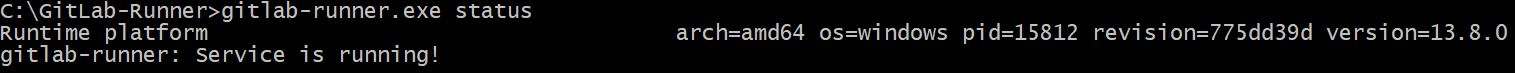
\includegraphics[width=1\textwidth, frame]{./grafiken/gitlab_runner_status.JPG}
	}
	\vskip0pt
	\caption{GitLab Runner Instanz auf einem lokalen Windows-Rechner}
\end{figure}

\subsection{Executors} \label{sssec:lblExecutor}

Wenn Sie einen Runner registrieren, müssen Sie einen Executor auswählen. Ein Executor bestimmt die Umgebung, in der jeder Job läuft.\autocite{gitlabRunner}

Wenn man zum Beispiel will, dass ein CI/CD-Auftrag PowerShell-Befehle ausführt, kann man GitLab Runner auf einem Windows-Server installieren und dann einen Runner registrieren, der den Shell-Executor verwendet.
Wenn man möchte, dass ein CI/CD-Job Befehle in einem benutzerdefinierten Docker-Container ausgeführt wird, muss man GitLab Runner auf einem Linux-Server installieren und einen Runner registrieren, der den Docker-Executor verwendet.
Dies sind nur einige der möglichen Konfigurationen. Man könnte GitLab Runner auch auf einer virtuellen Maschine installieren und eine andere virtuelle Maschine als Executor verwenden lassen.
Wenn man GitLab Runner in einem Docker-Container installieren und den Docker-Executor für die Ausführung der Jobs auswählen, wird dies manchmal als "Docker-in-Docker"-Konfiguration bezeichnet.\autocite{gitlabRunner}

\subsection{Shared Runners}

Shared Runners sind für jedes Projekt in einer GitLab-Instanz verfügbar.

Shared Runners werden verwendet, wenn man mehrere Jobs mit ähnlichen Anforderungen in mehreren Projekten hat. Also anstatt viele Runner für viele Projekte im Leerlauf zu haben, kann man eine Gruppe von Runner für alle Projekte benützen.\autocite{gitlabSharedRunner}

\subsection{Tags}

Registrierte Runner kann man sogenannte Tags zuweisen. Wenn ein CI/CD Job läuft, kann dieser anhand seiner zugewiesener Tags determinieren, welchen Runner er verwenden soll. Das hat den Vorteil, dass man für beispielsweise einen Job, der ein Ruby Projekt kompilieren soll, seinen Runner nicht umkonfigurieren muss, sondern automatisch der Ruby-Runner verwendet wird.

Man muss dazu lediglich folgendes in seine \texttt{.gitlab-ci.yml} Datei einbinden:

\begin{figure}[H]
	\centerline{
		
\includegraphics[width=1\textwidth, frame]{./grafiken/ruby_runner_tag_in_gitlab-ci-yml_file.JPG}
	}
	\vskip0pt
	\caption{ruby Tag in gitlab-ci.yml Datei (Bild wurde entnommen aus \autocite{gitlabRunner})}
\end{figure}

\section{MyPöttinger GitLab Pipeline}

Die Umgestaltung der GitLab Pipeline für das MyPöttinger-Repository ist ein wichtiger Bestandteil der Diplomarbeit. Die neue Pipeline besteht aus drei Stages:

\begin{itemize}
	\item Der \texttt{Build-Stage}
	\item Der \texttt{Test-Stage}
	\item Der \texttt{Release-Stage}
	\item Der \texttt{Image-Stage}
\end{itemize}

\subsection{Die {\texttt{gitlab-ci.yml}} - Datei }

Die \texttt{gitlab-ci.yml} Datei ist in GitLab hauptverantwortlich für die CI/CD Abläufe. Sie beschreibt die Aufgaben der einzelnen Jobs, definiert in welcher Stage diese auszuführen sind und legt die Reihenfolge der Abarbeitung klar fest. Bevor man sich über die \texttt{gitlab-ci.yml} Datei Gedanken macht, ist es wichtig, auf mehrere Aspekte zu achten. Man muss sich überlegen, welchen Runner [\ref{sec:lblGitLabRunner}] man verwenden will, welchen Executor [\ref{sssec:lblExecutor}] dieser ausführt und in welcher Umgebung alles stattfindet.

Zu Beginn der \texttt{gitlab-ci.yml} Datei muss man definieren, in welcher Umgebung Befehle ausgeführt werden sollen. Für MyPöttinger ist standardmäßig das \texttt{mcr.microsoft.com\\/dotnet/sdk:5.0} Image von Microsoft gewählt, da diese bereits .NET CLI, .NET runtime und ASP.NET Core bereit stellt, welche alle für das Kompilieren, Bauen und Veröffentlichen einer .NET-Applikation benötigt werden.

\begin{lstlisting}[caption={Erste Zeilen der gitlab-ci.yml Datei}, language=yaml, label={lst:lstErsteZeilen}]
	default:
		image: mcr.microsoft.com/dotnet/sdk:5.0
	variables:
		ENTRYPOINT_DLL: Tevaluator.dll
		DOCKER_IMAGE_VERSION: latest
	cache:
		paths:
		- src/MyPoettinger.App/node_modules/
	stages:
		- build
		- test
		- release
		- images
\end{lstlisting}

Jetzt wird das Listing~\ref{lst:lstErsteZeilen} beschrieben. Am Start ist die Definition der standardmäßigen Umgebung, welche mit \texttt{image:} angegeben wird. 

Der \texttt{cache:} Befehl ermöglicht es, Dateien oder Verzeichnisse, welche im Laufe der Pipeline-Jobs im angegebenen Ordner erzeugt wurden, zu speichern, um diese im weiteren Verlauf zu verwenden.

Die einzelnen Stages werden mit \texttt{stages:} deklariert. Alle folgenden Jobs können nun zu einer der aufgelisteten Stages hinzugefügt werden und laufen in dieser Reihenfolge ab.

\subsection{Die Build-Stage}\label{sssec:lblBuildStage}

\begin{lstlisting}[caption={Die Build-Stage der gitlab-ci.yml Datei}, language=yaml, label={lst:lstBuildStage}]
	build_dotnet:
		stage: build
		script:
		- dotnet restore --no-cache --force src/MyPoettinger.sln
		- dotnet build -c Release --no-restore src/MyPoettinger.sln
  		artifacts:
			paths:
			- test
			expire_in: 1 hour
		tags:
		- e
	
	build_angular:
		stage: build
		image: trion/ng-cli:10.0.4
		script: 
		- cd src/MyPoettinger.App
		- npm install
		- npm audit fix
		tags:
		- e
\end{lstlisting}

Da die Diplomarbeit aus einem Angular-Frontend (\texttt{src/MyPoettinger.App}) und einem .NET Backend (\texttt{src/MyPoettinger.sln}) besteht, müssen zwei unterschiedliche Projekte in dieser Stage zusammengebaut werden. 

Jetzt wird das Listing~\ref{lst:lstBuildStage} beschrieben. Bei dem \texttt{build\_dotnet} Job wird am Anfang \texttt{dotnet restore} ausgeführt, welcher mithilfe von NuGet die Abhängigkeiten des Projektes wieder herstellt. 

Der \texttt{dotnet build}-Befehl erstellt das Projekt und die zugehörigen Abhängigkeiten in einen Satz von Binärdateien. Die Binärdateien enthalten den Projektcode in IL-Dateien (Intermediate Language) mit der Erweiterung DLL. Abhängig vom Projekttyp und den Einstellungen können auch andere Dateien enthalten sein.\cite{dotnetBuildDesc} Im Anschluss des Vorgangs wird das Test-Verzeichnis als Artefakt gespeichert, um dieses anschließend in der Test-Stage zu testen.

Durch den Node Package Manager, kurz \texttt{npm}, werden mit dem Befehl \texttt{npm install} alle benötigten Pakete für das Angular Projekt heruntergeladen und installiert. Da allerdings im zuvor standardmäßig definierten dotnet-Image kein Node installiert ist, wechseln wir in \texttt{build\_angular} auf das \texttt{trion/ng-cli:10.0.4} Image, da es sich hier um eine sehr kleine Node-Umgebung handelt. Im folgenden Schritt wird mit \texttt{npm audit fix} erörtert, welche Pakete mögliche Sicherheitsrisiken darstellen. Diese werden danach automatisch behoben. 

\subsection{Die Test-Stage}

\begin{lstlisting}[caption={Die Test-Stage der gitlab-ci.yml Datei}, language=yaml, label={lst:lstTestStage}]
	unit_tests:
		stage: test
		script: 
		- dotnet test test/MyPoettinger.UnitTests/bin/Release/
		   net5.0/MyPoettinger.UnitTests.dll
		rules:
		- exists:
		  - test/*UnitTests/*UnitTests.csproj
		tags:
		- i  
	
	integration_tests:
		stage: test
		script: 
		- dotnet test test/MyPoettinger.IntegrationTests/bin/Release/
		   net5.0/MyPoettinger.IntegrationTest
		rules:
		- exists:
		  - test/*IntegrationTests/*IntegrationTests.csproj
		tags:
		- i
\end{lstlisting}

In der Test-Stage, welche im Listing~\ref{lst:lstTestStage} dargestellt wird, werden die Artefakte, welche bei der Build-Stage [\ref{sssec:lblBuildStage}] erzeugt wurden, geladen. Somit entsteht für die Jobs die Möglichkeit, das Test-Verzeichnis zu laden und die Tests mit \texttt{dotnet test} auszuführen. Hier wurde auch eine Regel eingeführt, diese Jobs nur dann auszuführen, wenn das angegebene Verzeichnis existiert. 


\subsection{Die Release-Stage}

\begin{lstlisting}[caption={Die Release-Stage der gitlab-ci.yml Datei}, language=yaml, label={lst:lstReleaseStage}]
	publish_dotnet:
		stage: release
		script:
		- dotnet publish src/MyPoettinger.sln -c Release
		artifacts:
		  name: DotArtifact
		  expire_in: 1 hour
		  paths:
		  - /builds/it-entwicklung/dotnet
		    /mypoettinger/src/MyPoettinger.Web/bin
		    /Release/netcoreapp3.1/publish/
		tags:
		- e
		
	publish_angular:
		stage: release
		image: trion/ng-cli-karma:9.0.1
		script:
		- cd src/MyPoettinger.App
		- ng build --prod --aot=true
		artifacts:
	  	  name: AngularArtifact
		  expire_in: 1 day
		  paths:
		  - src/MyPoettinger.App/dist
		tags:
		- e
\end{lstlisting}

\colorbox{MyLightGrayBackgroundForCode}{\texttt{dotnet publish}} kompiliert die Anwendung, liest ihre Abhängigkeiten, die in der Projektdatei angegeben sind, und veröffentlicht die resultierenden Dateien in einem Verzeichnis. Die Ausgabe umfasst die folgenden Objekte:\cite{dotnetpublish}

\begin{itemize}
	\item Intermediate Language-Code (IL) in einer Assembly mit einer \textit{DLL}-Erweiterung
	\item Die Datei \textit{.deps.json}, die alle Abhängigkeiten des Projekts enthält
	\item Die Datei \textit{.runtimeconfig.json}, die die Shared Runtime, die von der Anwendung erwartet wird, sowie andere Konfigurationsoptionen für die Runtime festlegt (z. B. die Art der Garbage Collection).
	\item Die Abhängigkeiten der Anwendung, die aus dem NuGet-Cache in den Ausgabeordner kopiert werden.
\end{itemize}

Die Ausgabe des Befehls dotnet publish steht für die Bereitstellung zur Ausführung auf einem Hostsystem bereit (z.B. ein Server, Computer, Mac oder Laptop). Es ist die einzige offiziell unterstützte Methode zum Vorbereiten der Anwendung für die Bereitstellung. Je nach Art der Bereitstellung, die im Projekt angegeben ist, ist die Shared Runtime von .NET im Hostsystem installiert oder nicht.\cite{dotnetpublish} Die Artefakte dieses Jobs im Listing~\ref{lst:lstReleaseStage} kann man anschließend in einem Deploy-Job verwenden oder manuell von der GitLab Seite herunterladen.

Bei dem \texttt{publish\_angular} Job im Listing~\ref{lst:lstReleaseStage} wird wieder das \texttt{trion/ng-cli:10.0.4} Image verwendet, um auf eine Node-Umgebung zu wechseln. Der Job ladet automatisch die node\_modules aus dem Cache und verwendet diese, um aus der Angular-Applikation mit dem Befehl \colorbox{MyLightGrayBackgroundForCode}{\texttt{ng build --prod -aot=true}}, welcher im Hintergrund das \texttt{webpack build tool} verwendet, reine Javascript-Dateien zu erzeugen, welche wiederum an einen Deploy-Job weitergeleitet werden können oder manuell von der GitLab Seite heruntergeladen werden können, um diese lokal auszuführen.

\newpage

\subsection{Die Images-Stage}

\begin{lstlisting}[caption={Die Images-Stage der gitlab-ci.yml Datei}, language=yaml, label={lst:lstImagesStage}]
	containerize_dotnet:
		stage: images
		cache: {}
		image:
		name: gcr.io/kaniko-project/executor:debug
		entrypoint: [""]
		script:
		- echo "FROM mcr.microsoft.com/dotnet/sdk:5.0" > $CI_PROJECT_DIR/Dockerfile
		- echo "COPY src/MyPoettinger.Web/bin
			/Release/netcoreapp3.1/publish/ ." >> $CI_PROJECT_DIR/Dockerfile
		- echo "EXPOSE 80" >> $CI_PROJECT_DIR/Dockerfile
		- echo "ENTRYPOINT [\"dotnet\", \"$ENTRYPOINT_DLL\"]" >> $CI_PROJECT_DIR/Dockerfile
		
		- echo "{\"auths\":{\"$CI_REGISTRY\":{\"username\":
			\"$CI_REGISTRY_USER\",\"password\":
			\"$CI_REGISTRY_PASSWORD\"}}}" >
		 	/kaniko/.docker/config.json
		
		- /kaniko/executor --context $CI_PROJECT_DIR --dockerfile $CI_PROJECT_DIR/Dockerfile --destination $CI_REGISTRY_IMAGE:$DOCKER_IMAGE_VERSION
		tags:
		- i
		
	containerize_angular:
		stage: images
		image: docker:stable
		services:
		- docker:dind
		before_script:
		- docker login -u $CI_REGISTRY_USER -p $CI_REGISTRY_PASSWORD $CI_REGISTRY
		script:
		- echo "FROM nginx:latest" > $CI_PROJECT_DIR/Dockerfile
		- echo "COPY src/Tevaluator.App/dist/tevaluator /usr/share/nginx/html" >> $CI_PROJECT_DIR/Dockerfile
		- echo "COPY nginx.conf /etc/nginx/nginx.conf" >> $CI_PROJECT_DIR/Dockerfile
		- cat $CI_PROJECT_DIR/Dockerfile
		
		- IMAGE_NAME="$CI_REGISTRY_IMAGE/angularcontainer"
		- docker build --pull -t "$IMAGE_NAME" -f $CI_PROJECT_DIR/Dockerfile .
		- docker push "$IMAGE_NAME"
\end{lstlisting}

Beide Jobs, \texttt{containerize\_dotnet} und \texttt{containerize\_angular}, kümmern sich um den Abschluss der Continous Delivery. Ziel ist es, die Software in zwei unabhängige Docker-Images zu bündeln, um diese anschließen in die Container-Registry von GitLab zu pushen.

Um ein Docker-Image der gebündelten DotNet-Applikation zu  erstellen, wird im Job \texttt{containerize\_dotnet}, dargestellt im Listing~\ref{lst:lstImagesStage}, ein temporäres \texttt{Dockerfile} im Hauptverzeichnis der Applikation erstellt. Da die Angular-Jobs durchschnittlich 2 Minuten schneller sind als die Dotnet-Jobs, entstehen hier keine Probleme mit dem \texttt{containerize\_\\angular}-Job. Um das Image tatsächlich zu erstellen wird \textbf{\texttt{kaniko}} verwendet.

Das Kaniko-Executor-Image ist dafür verantwortlich, ein Image aus einem Dockerfile zu erstellen und es in eine Container-Registry zu schieben. Innerhalb des Kaniko-Executor-Image extrahieren wir das Dateisystem des Basisabbilds (das FROM-Abbild im Dockerfile). Anschließend führen wir die Befehle in dem Dockerfile aus und erstellen nach jedem Befehl einen Snapshot des Dateisystems im Userspace. Nach jedem Befehl wird eine Schicht mit geänderten Dateien an das Basis-Image angehängt (falls vorhanden) und die Metadaten des Images werden aktualisiert\cite{kaniko}. Kaniko ist nicht von einem Docker-Daemon abhängig und führt jeden Befehl innerhalb eines Dockerfiles vollständig im Userspace aus. Dies ermöglicht die Erstellung von Container-Images in Umgebungen, in denen ein Docker-Daemon nicht einfach oder sicher ausgeführt werden kann, wie z. B. in einem Standard-Kubernetes-Cluster.\cite{kaniko}

Das Dockerimage des Jobs holt sich das \texttt{mcr.microsoft.com/dotnet/sdk:5.0}-Image, kopiert die \texttt{publish\_dotnet}-Artefakte in das Hauptverzeichnis des Containers, öffnet den Port 80, um auf diesen von außen zugreifen zu können und führt die .dll-Datei aus.

Schlussendlich wird im \texttt{containerize\_angular}-Job das Dockerimage erstellt. Sowohl die \texttt{publish\_angular}-Artefakte, als auch die Konfigurationsdatei \texttt{nginx.conf}, werden in das \texttt{nginx:latest}-Image kopiert. Beim Start des Containers wird \texttt{nginx} automatisch ausgeführt.

Im Nachfolgenden Screenshot sieht man einen erfolgreich abgeschlossenen Pipeline-Durchgang:

\begin{figure}[H]
	\centerline{
		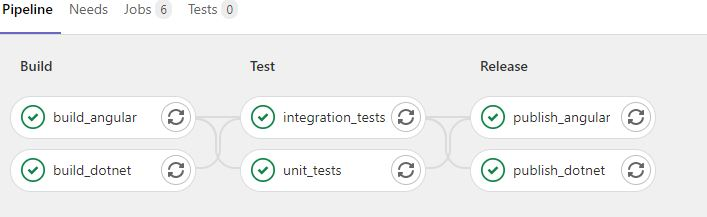
\includegraphics[width=1\textwidth, frame]{./grafiken/build_test_release_successful.JPG}
	}
	\vskip0pt
	\caption{Erfolgreicher Durchgang der Pipeline}
\end{figure}
	
	%%%%%%%%%%%%%%%%%%%%%%%%%%%%%%%%%%%%%%%%%
	%%%   BESCHREIBUNG AUS ANWENDERSICHT   %%
	%%%%%%%%%%%%%%%%%%%%%%%%%%%%%%%%%%%%%%%%%
	
	\chapter{Beschreibung aus Anwendersicht} \label{anwendersicht}
Dieses Projekt wurde für den Kunden entwickelt, daher wird im Folgenden die Anwendersicht beschrieben.
\section{Länderwahl}
\begin{figure}[H]
	\centerline{
		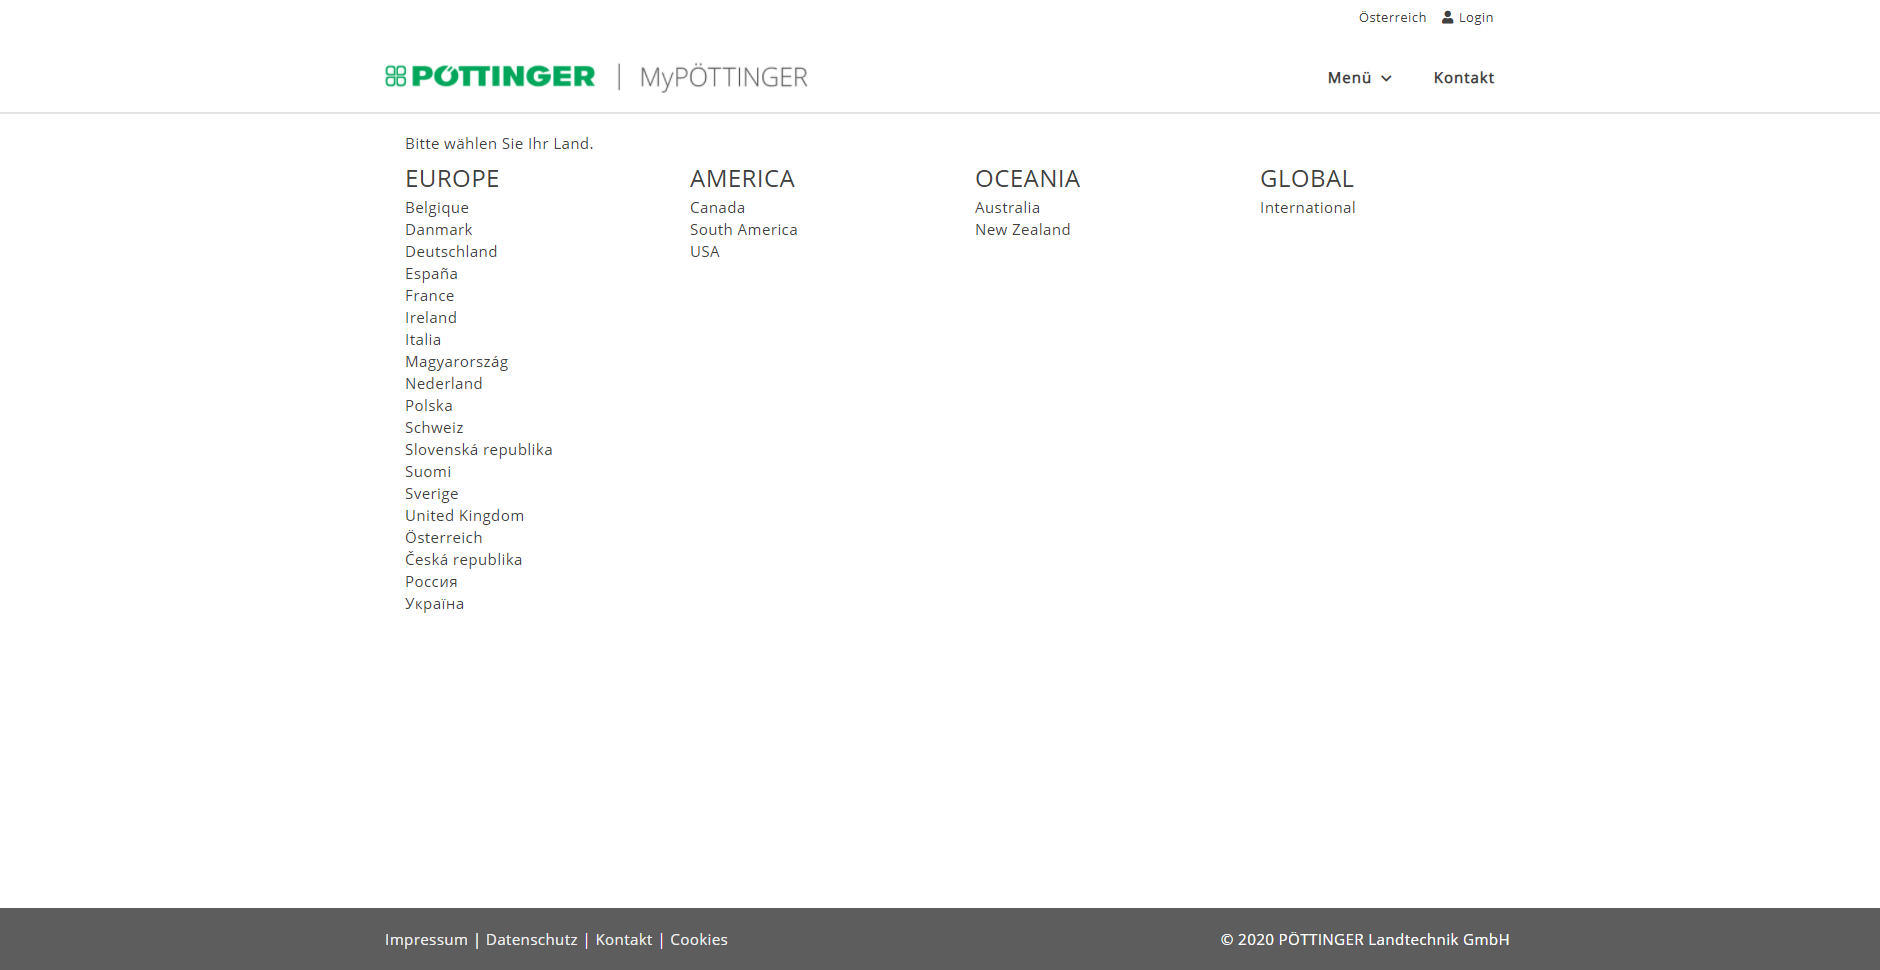
\includegraphics[width=1\textwidth, frame]{./grafiken/erm_country_selection.png}
	}
	\vskip0pt
	\caption{Screenshot der Länderwahl} \label{fig:countrySelection}
\end{figure}
Um auf die Webseite zu gelangen, ist es erforderlich, dass man davor in der Länderwahl, wie in Abbildung \ref{fig:countrySelection} gezeigt wird, sein Land wählt und bei den Ländern, in denen es mehrere Landessprachen gibt, auch die Sprache wählt. Aus dem Länder- und Sprachenkürzel setzt sich die Locale zusammen. Für Österreich wäre die Locale daher "de\_AT" und für Deutschland "de\_DE". Diese Locale wird in den Cookies gespeichert und die Webseite richtet sich nach dieser Locale in den Cookies. Es ist auch möglich, im Nachhinein das Land und die Sprache zu ändern, indem man im Header der Webseite auf das Land klickt. Durch diesen Klick gelangt man von überall auf die Länderwahl.

\section{Startseite}
\subsection{Startseite vor dem Login}
\begin{figure}[H]
	\centerline{
		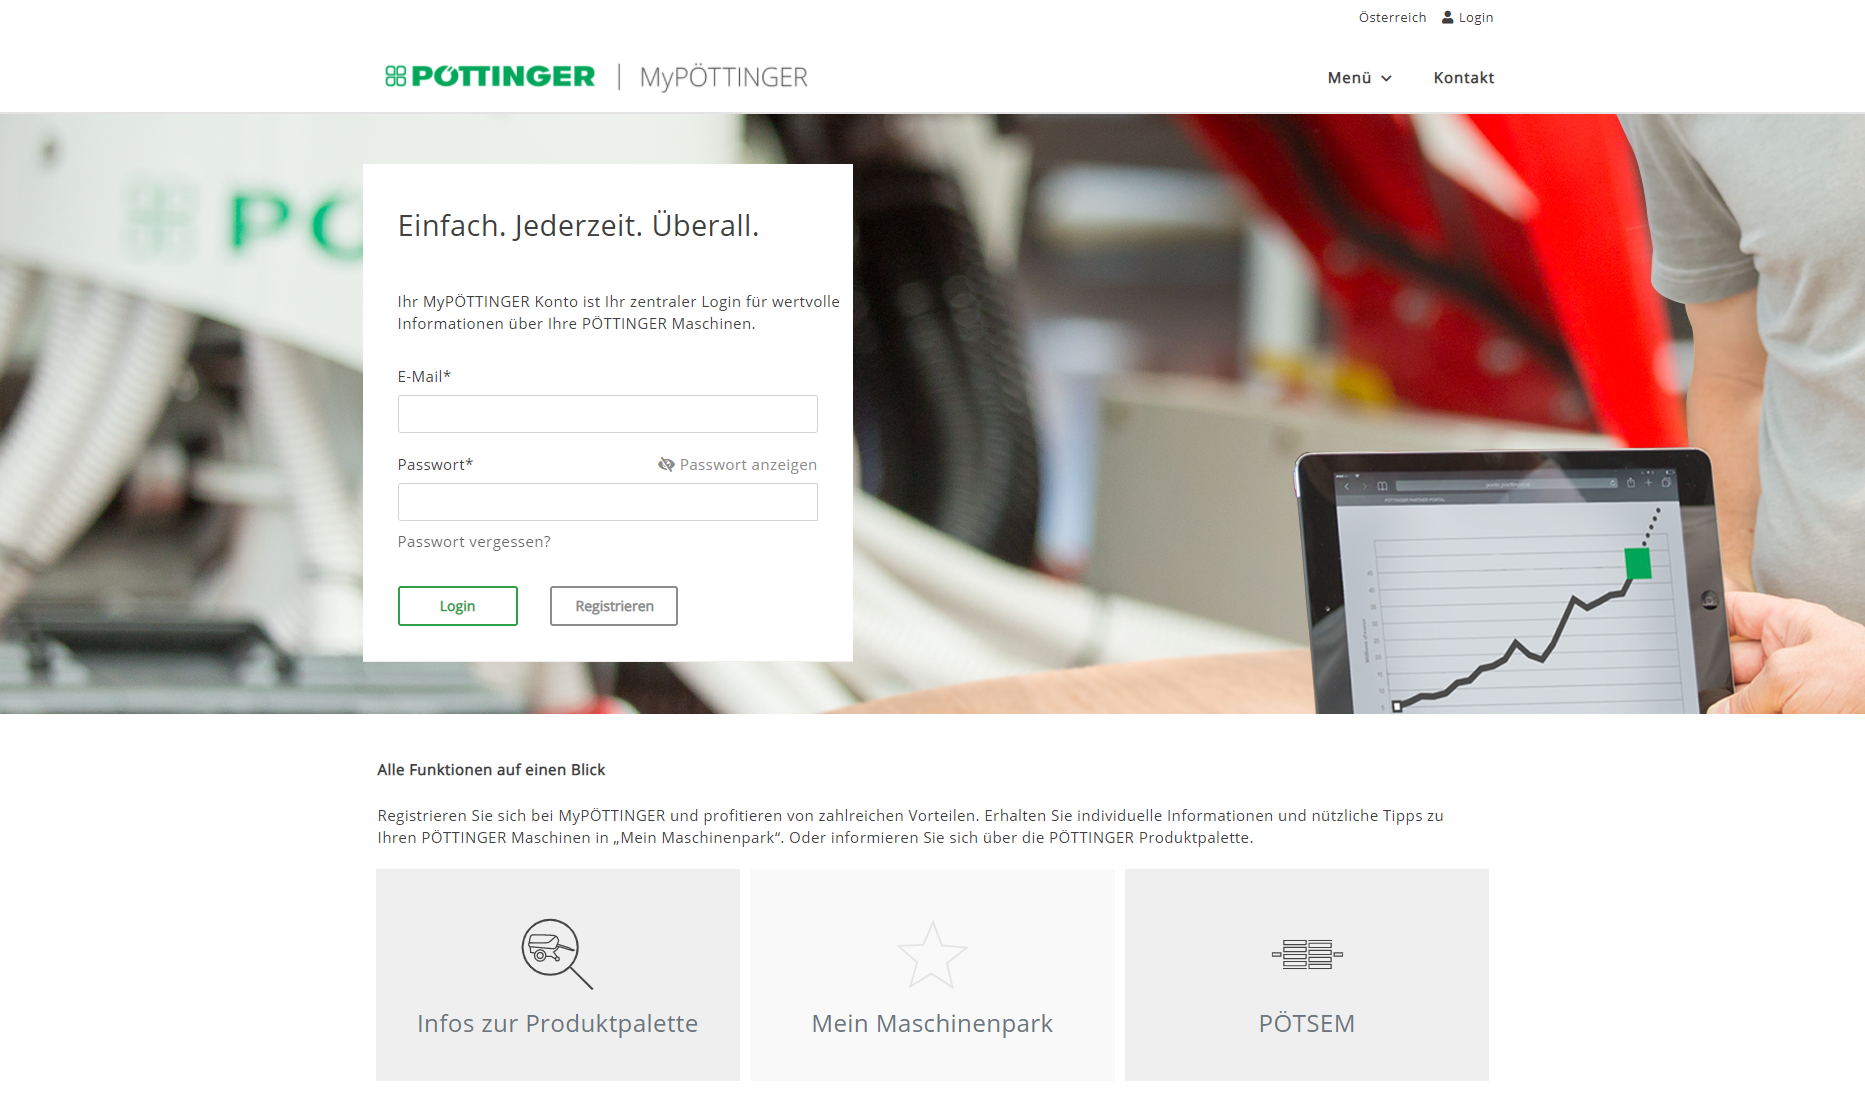
\includegraphics[width=1\textwidth, frame]{./grafiken/erm_home_not_logged_in_1.png}
	}
	\vskip0pt
	\caption{Screenshot von der Startseite nicht eingeloggt} \label{fig:homeNotLoggedIn}
\end{figure}

Nach der Länderwahl gelangt man auf die Startseite. Anfangs ist man noch nicht eingeloggt, daher ist ein Login-Feld in der Mitte, wie man in Abbildung \ref{fig:homeNotLoggedIn} sehen kann. Dort sieht man auch, dass das Feld "Mein Maschinenpark" etwas heller ist als die anderen Felder, da man den Maschinenpark nur als eingeloggter Benutzer verwenden kann. Die beiden anderen Felder sind auch ohne Registrierung nutzbar.
 
\subsection{Startseite nach einem erfolgreichen Login}
\begin{figure}[H]
	\centerline{
		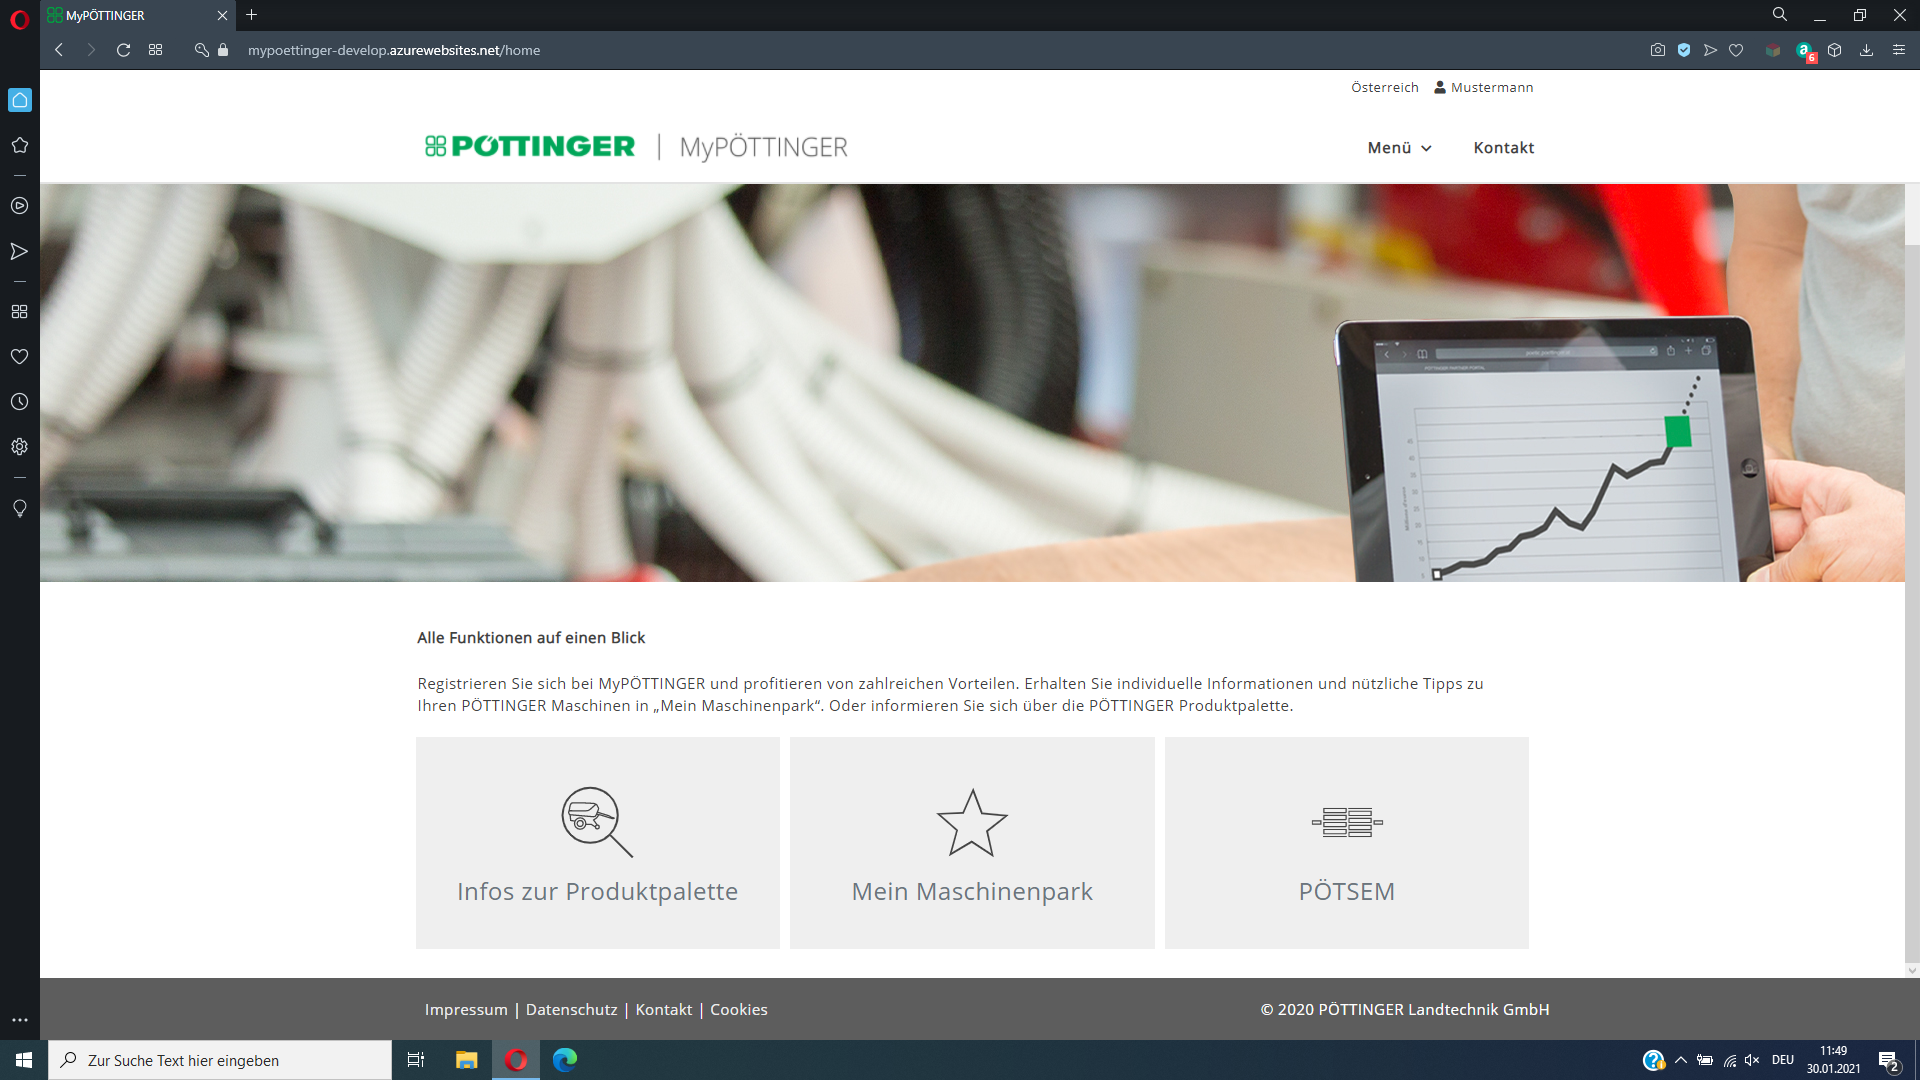
\includegraphics[width=1\textwidth, frame]{./grafiken/erm_home_logged_in.png}
	}
	\vskip0pt
	\caption{Screenshot von der Startseite eingeloggt} \label{fig:homeLoggedIn}
\end{figure}

Nach einem erfolgreichen Login ist das Feld "Mein Maschinenpark" aktiv. Als eingeloggter Benutzer hat man nun Zugriff auf den Maschinenpark. Das erkennt man daran, dass das Feld in Abbildung \ref{fig:homeLoggedIn} den selben Grauton hat, wie die beiden anderen Felder. 

\section{Registrierungsseite}

Falls man noch nicht registriert ist und man auf der Startseite auf "Registrieren" drückt, wird man zur Registrierungsseite weitergeleitet. Den ersten Teil dieser Seite sieht man in Abbildung \ref{fig:register}.

\subsection{Registrierung}
\begin{figure}[H]
	\centerline{
		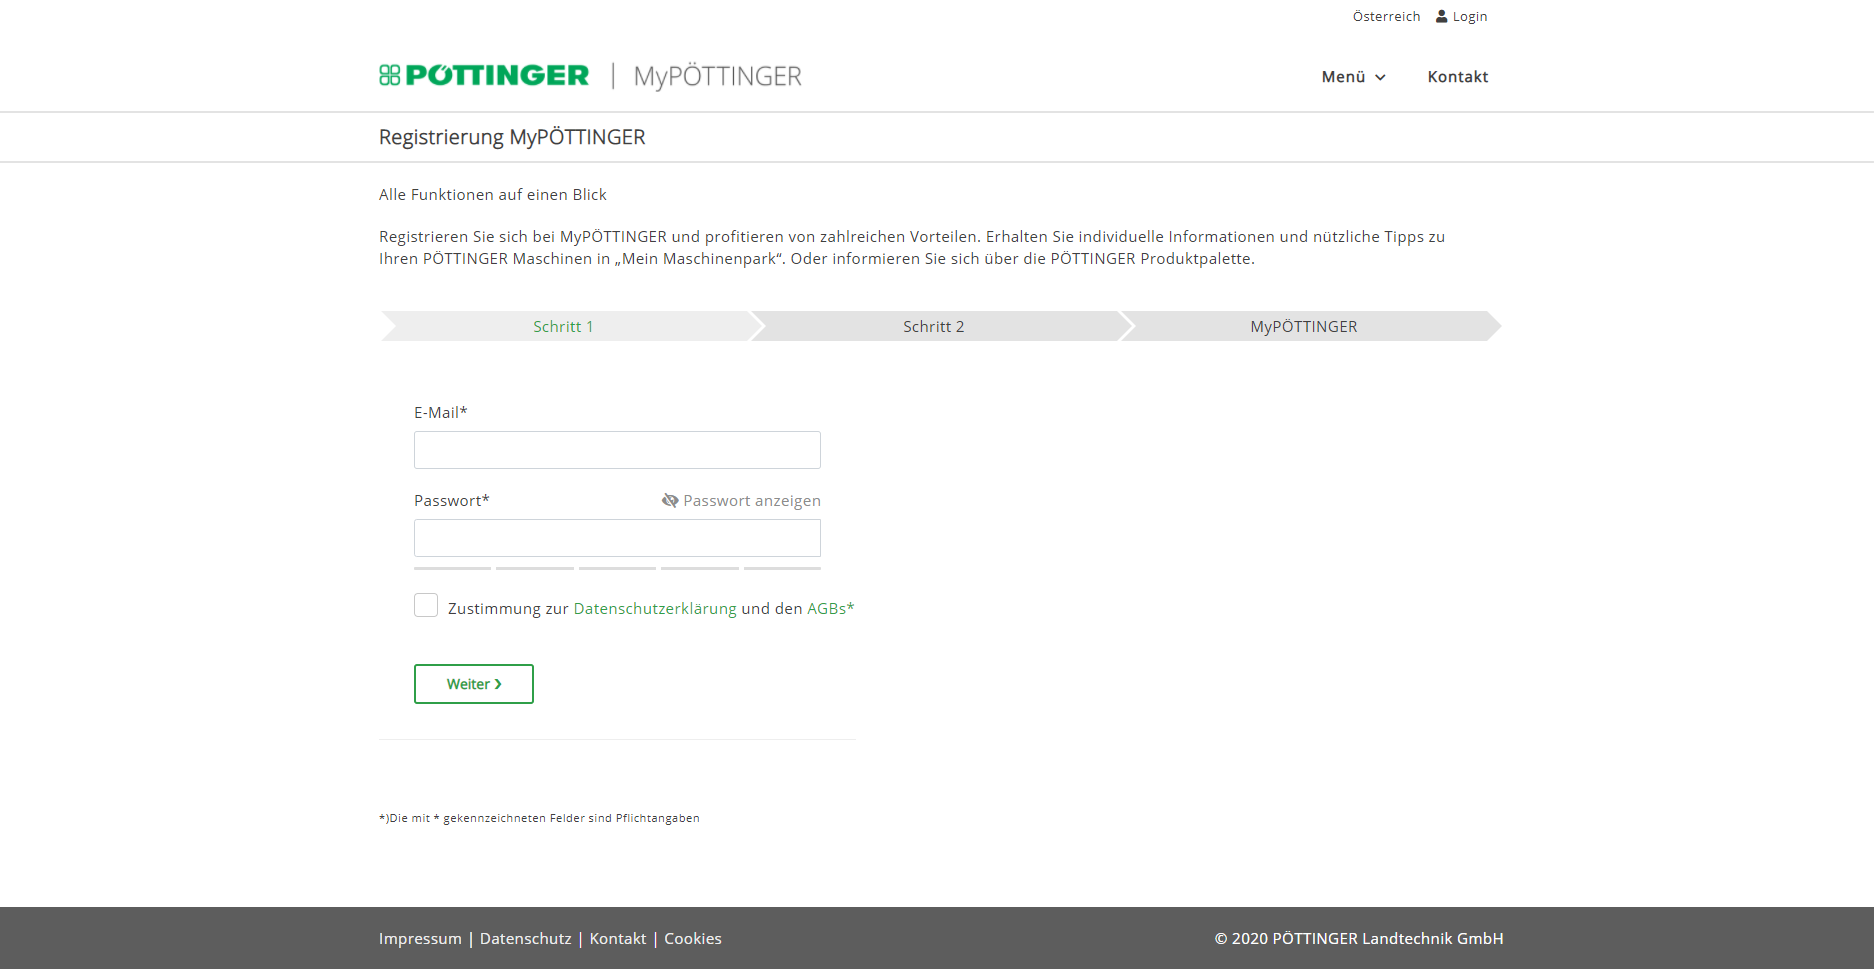
\includegraphics[width=1\textwidth, frame]{./grafiken/erm_register.png}
	}
	\vskip0pt
	\caption{Screenshot von der Registrierungsseite} \label{fig:register}
\end{figure}

Während der Passworteingabe bekommt man Feedback, wie sicher das ausgewählte Passwort ist und ob noch Komponenten fehlen, um den Passwortanforderungen zu entsprechen. Die Passwortanforderungen, die man in Abbildung \ref{fig:pwHints} sieht, entsprechen den Voraussetzungen von Auth0, da die Registrierung über Auth0 läuft. Der Balken unter dem Passwortfeld, wie in Abbildung \ref{fig:pwSec} sichtbar, gibt die Sicherheit des Passwortes an. Das Passwort wird mit gängigen Namen und Nachnamen aus Amerika, beliebten englischen Wörtern und Mustern wie Datumsangaben, Wiederholungen und Tastaturmustern verglichen, um die Stärke angeben zu können.

\begin{figure}[H]
	\centerline{
		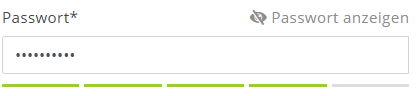
\includegraphics[width=1\textwidth, frame]{./grafiken/passwordSecurity.PNG}
	}
	\caption{Screenshot von der Passwortsicherheit} \label{fig:pwSec}
\end{figure}
\begin{figure}[H]
	\centerline{
	
\includegraphics[width=1\textwidth, frame]{./grafiken/passwordHints.PNG}
	}	
	\caption{Screenshot von den Passworthinweisen} \label{fig:pwHints}
\end{figure}

\subsection{Weitere Daten für die Registrierung} \label{sec:weitereDatenfuer}

In diesem Schritt der Registrierung füllt man persönliche Daten aus. Das Land und die Sprache werden von der am Beginn ausgewählten Locale übernommen. Diese kann man aber auch hier noch ändern. Wenn das Land oder die Sprache geändert wird, wird dieses Formular neu generiert und die Felder werden nach dem Standard des Landes erzeugt. Das bedeutet, dass die Reihenfolge der angezeigten Felder von dem ausgewählten Land abhängt, da in gewissen Ländern in einem Formular der Nachname vor dem Vornamen steht oder in bestimmten Ländern Staaten oder Provinzen dazu kommen. Die Feldbeschreibung wird auch nach der ausgewählten Sprache geändert. Weiters wird auch die Validierung der Felder angepasst, da zum Beispiel die Postleitzahl in den verschiedenen Länder variiert (4-stellig in Österreich, 5-stellig in Deutschland). \\
Für die Adresseingabe in der Abbildung \ref{fig:register2} hat der Benutzer 3 Möglichkeiten:\\
Es besteht die Möglichkeit, jedes Adressfeld selbst auszufüllen. Somit sind die Felder Straße und Hausnummer, Ort, Postleitzahl und bei gewissen Ländern außerdem die Provinzen oder Staaten auszufüllen.\\
Eine etwas schnellere Variante ist die Verwendung von dem integrierten Typeaheads. Bei der Eingabe in das Feld Straße und Hausnummer erscheinen Adresseingabevorschläge darunter. Wenn man auf die gewünschte Adresse klickt, werden die Felder Ort, Postleitzahl und falls vorhanden, die Provinz oder der Staat automatisch ausgefüllt. Alle angezeigten Vorschläge sind in dem ausgewählten Land. Somit wird verhindert, dass der Benutzer eine Adresse eingibt, die sich nicht in dem gewählten Land befindet.\\
Die schnellste Variante ist die Verwendung von der integrierten Standorterkennung. Dafür drückt man "Use my location" über dem Adressfeld. Dadurch wird der Standort bestmöglich erfasst und alle vorhandenen Adressfelder werden automatisch ausgefüllt. Falls der Standort nicht ganz richtig erkannt wurde, kann man diesen anschließend noch bearbeiten. Die Standorterkennung ändert auch das ausgewählte Land, falls dieses nicht übereinstimmt.
\begin{figure}[H]
	\centerline{
		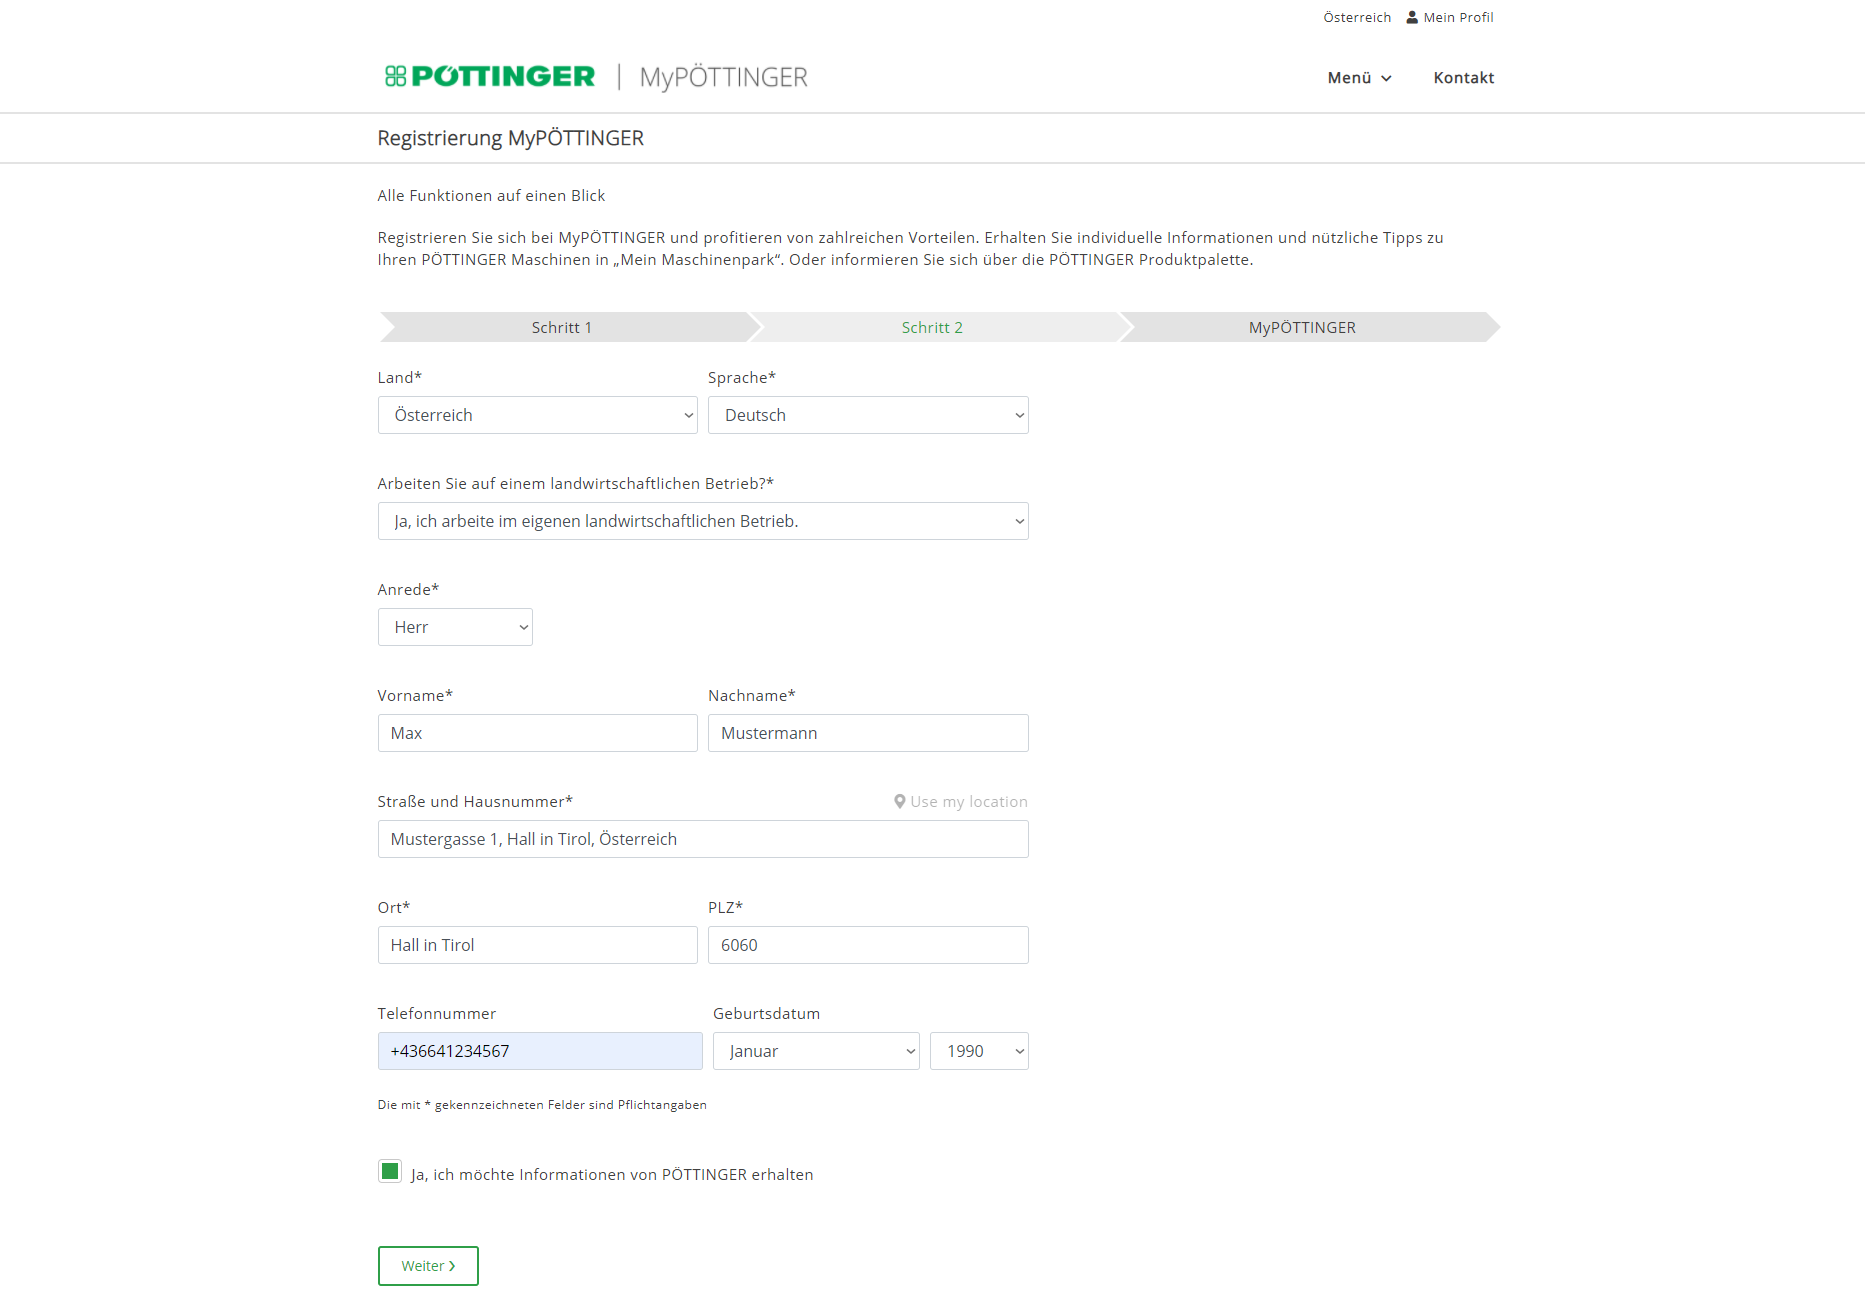
\includegraphics[width=1\textwidth, frame]{./grafiken/erm_register_data.png}
	}
	\vskip0pt
	\caption{Screenshot von der Dateneingabe der Registrierung} \label{fig:register2}
\end{figure}

Um anzugeben, ob der Benutzer auf einem landwirtschaftlichen Betrieb arbeitet, besteht die Möglichkeit auszuwählen, dass er auf dem eigenen landwirtschaftlichen Betrieb arbeitet, auf einem anderen landwirtschaftlichen Betrieb angestellt ist oder, dass er auf keinem Betrieb arbeitet. Falls der Benutzer auswählt, dass er auf einem anderen Betrieb angestellt ist, erscheint zusätzlich das Feld für den Namen des Unternehmens.\\
Jedes Eingabefeld wird sofort nach Abgabe des Cursorfokus validiert. Falls ein Fehler auftritt, wird das Feld rot umrandet und unter dem Feld erscheint eine Fehlermeldung, die angibt was falsch ist. Die Eingaben werden im Frontend und im Backend validiert. In der Abbildung \ref{fig:eingabeError} sieht man die Felder mit einigen möglichen Fehlermeldungen. Bei einer korrekten Eingabe verschwindet der rote Rahmen um das jeweilige Feld wieder.
\begin{figure}[H]
	\centerline{
		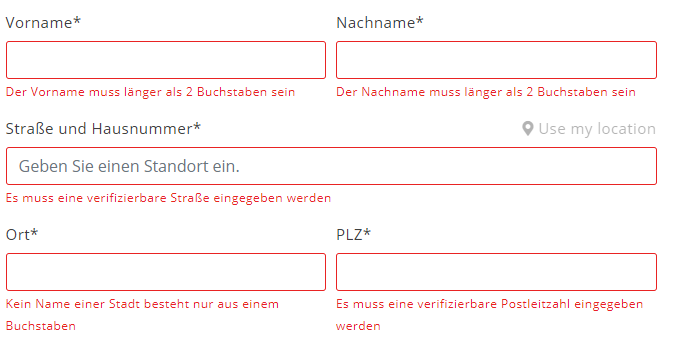
\includegraphics[width=1\textwidth, frame]{./grafiken/dateneingabe_Errors.PNG}
	}
	\vskip0pt
	\caption{Screenshot von den Fehlermeldungen der Eingaben} \label{fig:eingabeError}
\end{figure}

\subsection{Letzter Schritt der Registrierung}
Um die Registrierung erfolgreich abzuschließen, bekommt der User eine Bestätigung per E-Mail zugesendet. Darin befindet sich ein Aktivierungslink. Der letzte Schritt der Registrierung wird in der Abbildung \ref{fig:step3register} angezeigt. Hier wird man nur mehr gebeten, den Link in der E-Mail zu klicken. Nach der Aktivierung ist die Webseite ohne Einschränkungen nutzbar.
\begin{figure}[H]
	\centerline{
		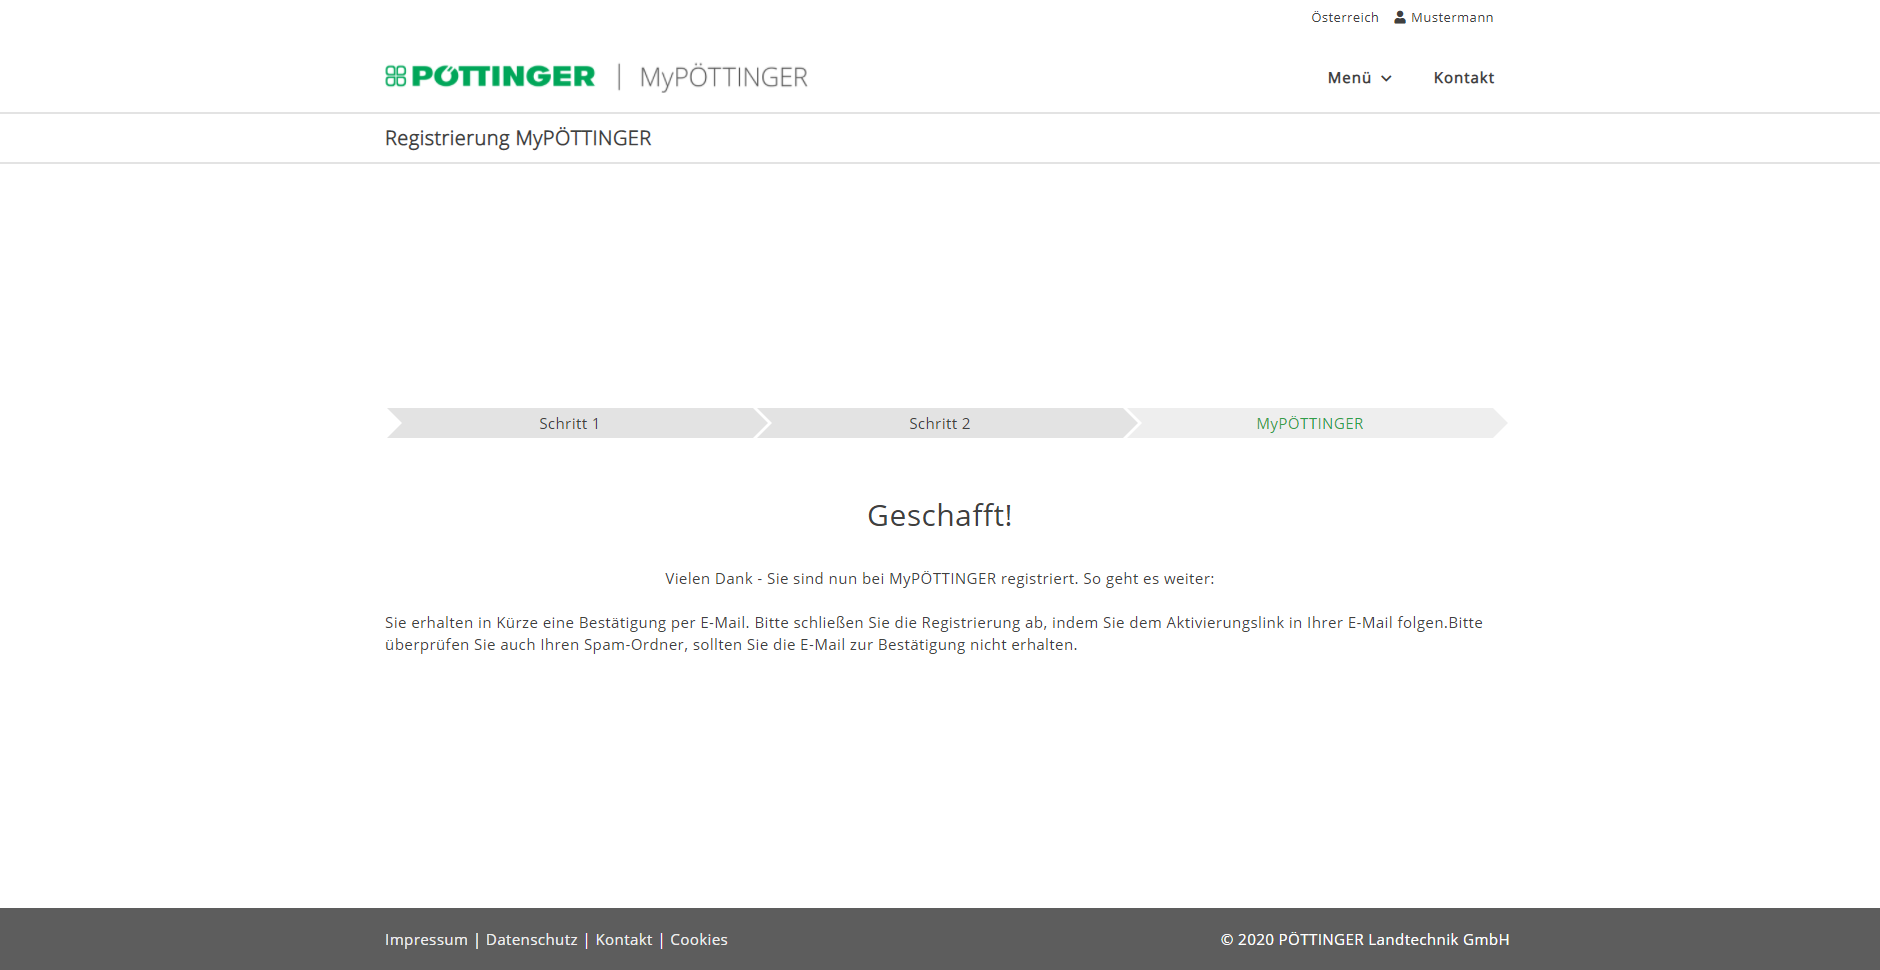
\includegraphics[width=1\textwidth, frame]{./grafiken/erm_register_final.png}
	}
	\vskip0pt
	\caption{Screenshot vom letzten Schritt der Registrierung} \label{fig:step3register}
\end{figure}

Nach der Bestätigung in der E-Mail wird man zurück auf die Startseite geleitet und es erscheint ein Pop-Up, wie die Abbildung \ref{fig:popup} zeigt.

\begin{figure}[H]
	\centerline{
		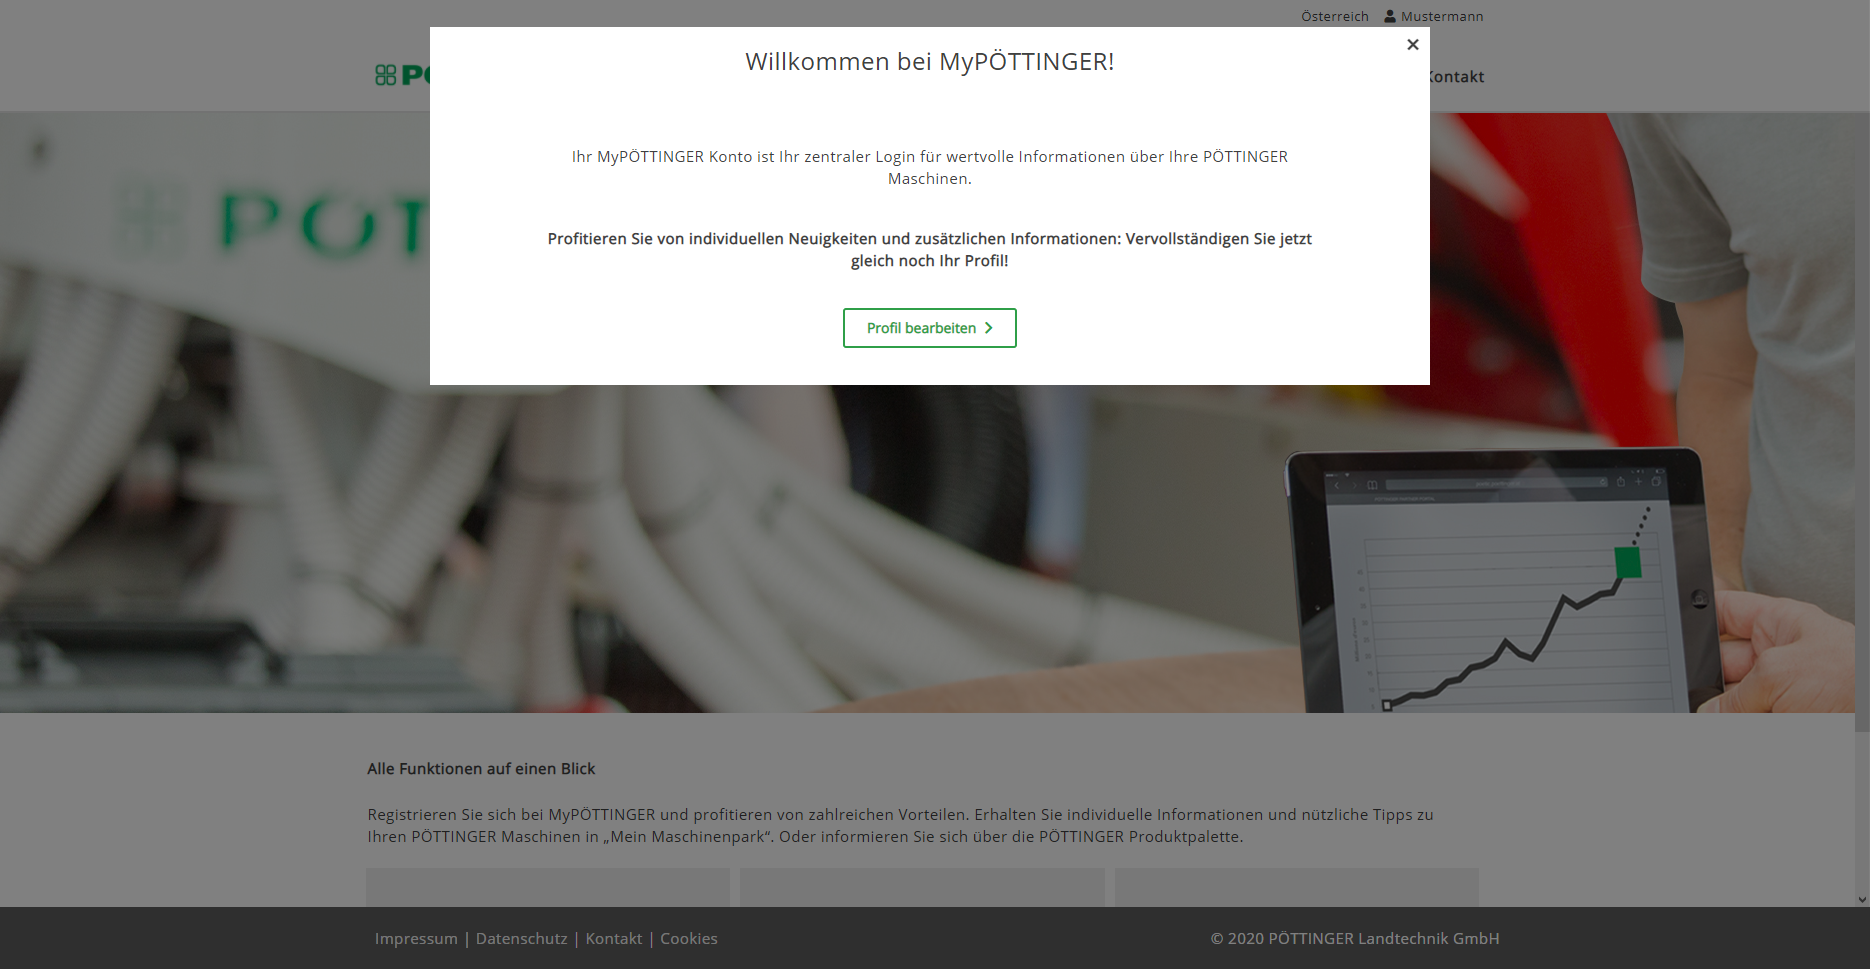
\includegraphics[width=1\textwidth, frame]{./grafiken/erm_home_after_email.png}
	}
	\vskip0pt
	\caption{Screenshot von dem Bestätigungs-Pop-Up} \label{fig:popup}
\end{figure}

\section{Profilübersicht}

Auf die Profilübersicht gelangt man, wenn man in dem Bestätigungs-Pop-Up auf "Profil bearbeiten" klickt oder auf den eigenen Namen rechts oben und direkt danach auf "Mein Profil". Die Profilübersicht sieht man in Abbildung \ref{fig:profil}.

\begin{figure}[H]
	\centerline{
		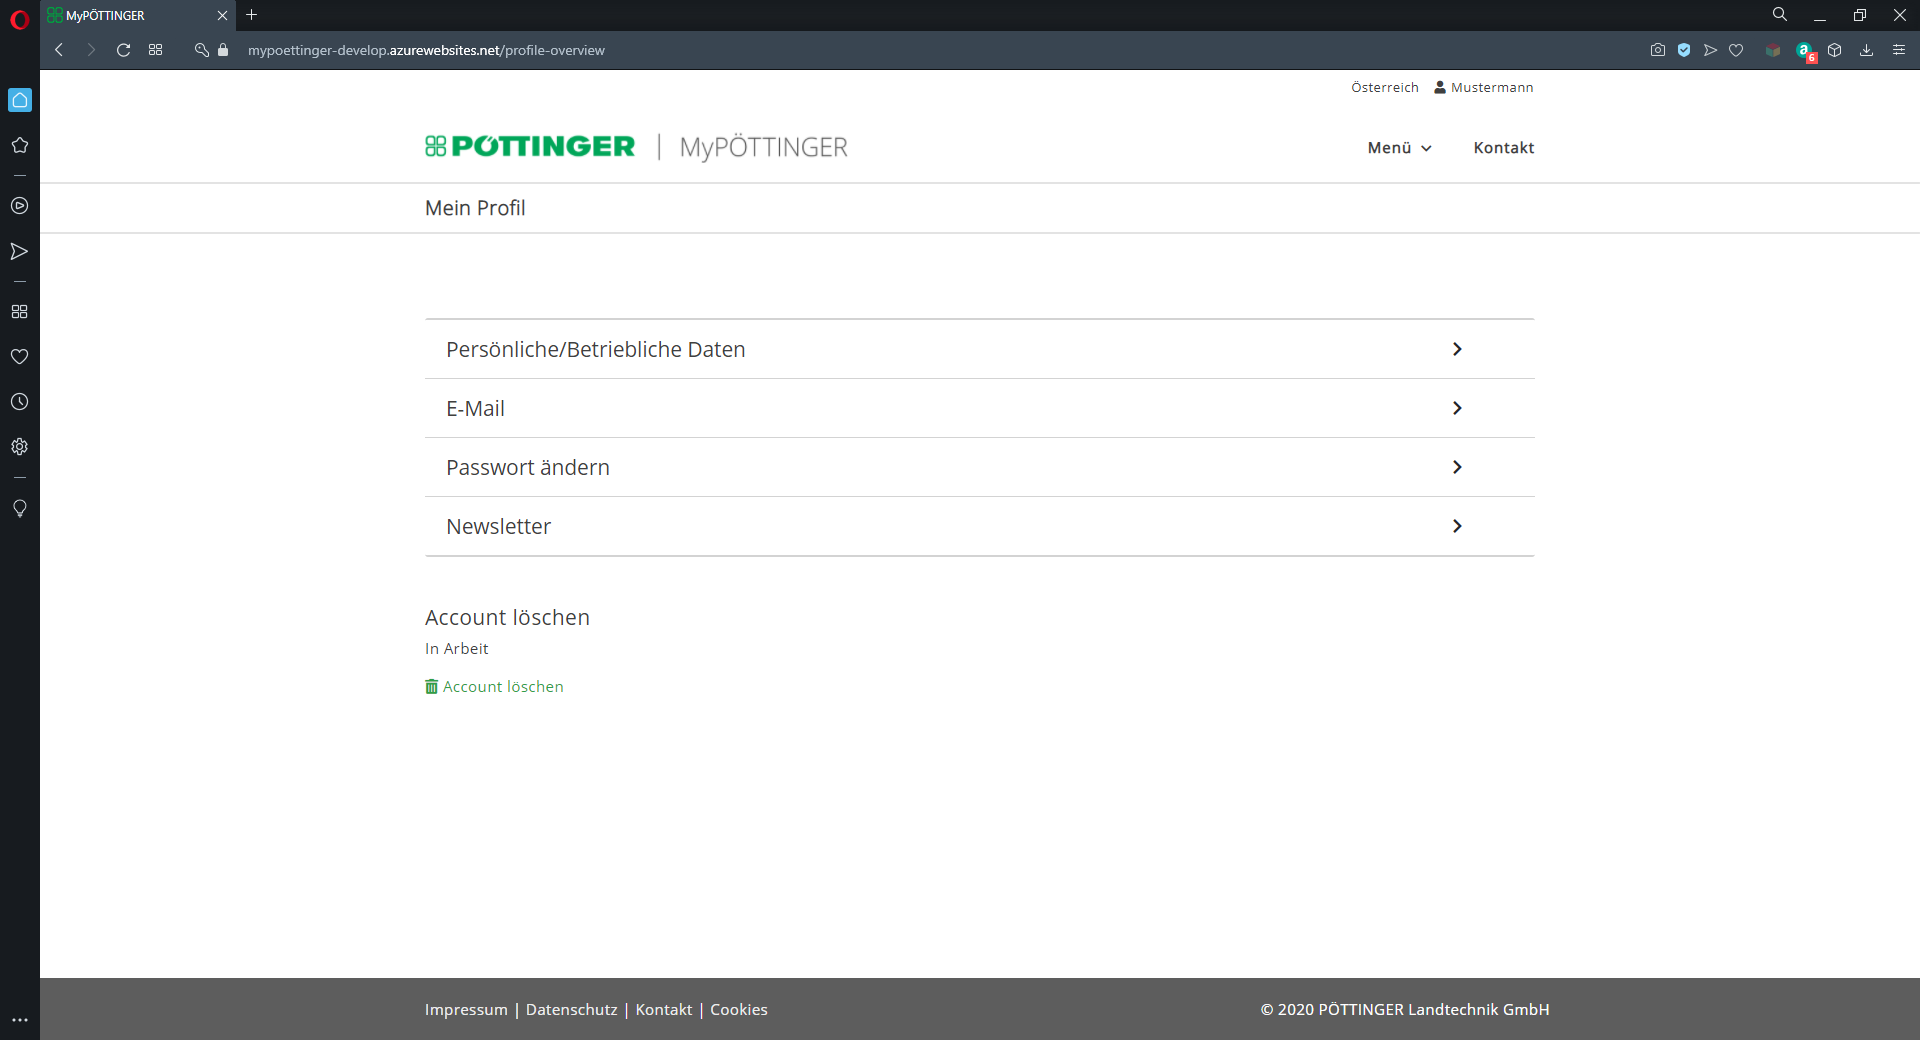
\includegraphics[width=1\textwidth, frame]{./grafiken/erm_profil.png}
	}
	\vskip0pt
	\caption{Screenshot von der Profilübersicht} \label{fig:profil}
\end{figure}

In der Profilübersicht kann man all seine persönlichen Daten einsehen und diese auch bearbeiten. Es besteht auch die Möglichkeit, die E-Mail und das Passwort zu ändern.

\subsection{Persönliche/Betriebliche Daten}

Nach der Registrierung ist es möglich, hier noch weiter persönliche und betriebliche Daten einzutragen. Falls der Benutzer ausgewählt hat, dass er auf dem eigenen oder einem anderen landwirtschaftlichen Betrieb arbeitet, erweitern sich die Dateneingabefelder um einige Felder für den Betrieb. Bei einem Klick auf "Persönliche/Betriebliche Daten" klappt sich ein Datenformular auf, dass man in Abbildung \ref{fig:profilData} sehen kann.

\begin{figure}[H]
	\centerline{
		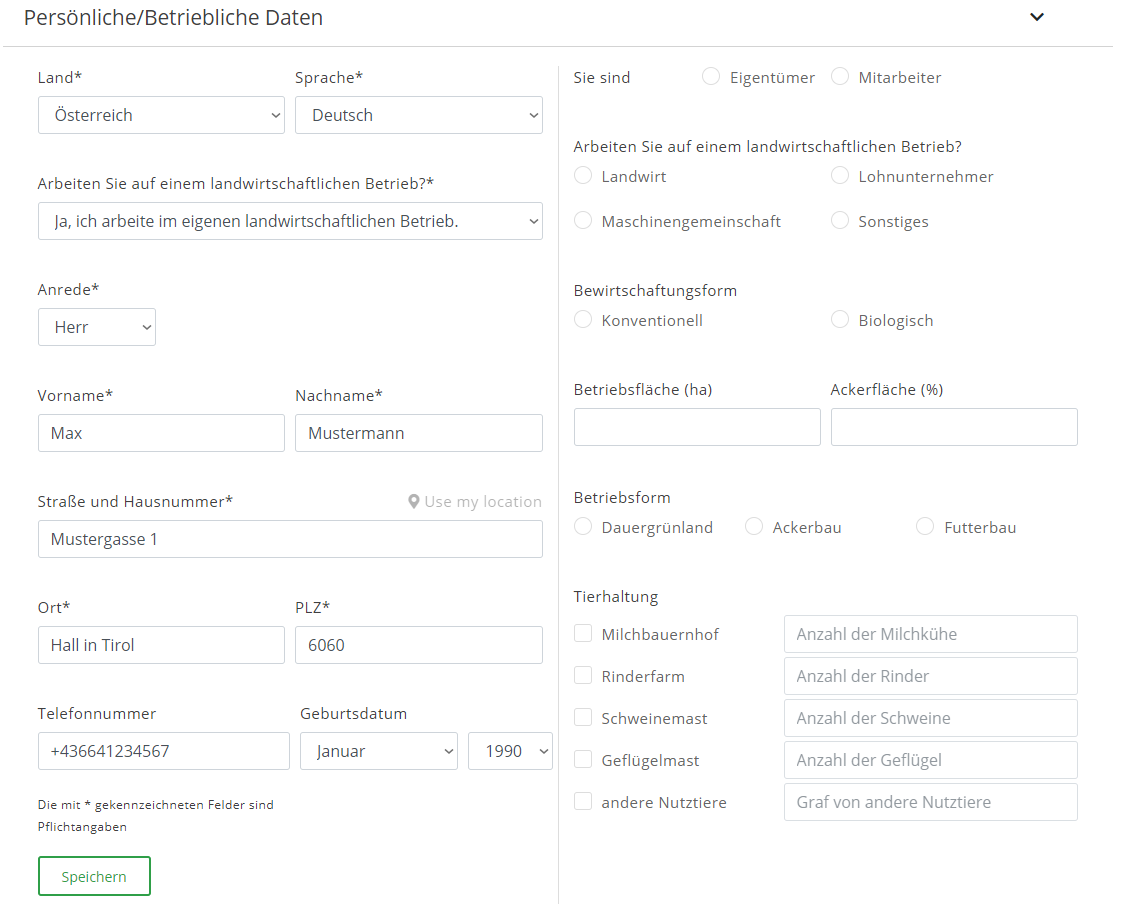
\includegraphics[width=1\textwidth, frame]{./grafiken/erm_profil_daten.png}
	}
	\vskip0pt
	\caption{Persönliche/Betriebliche Daten} \label{fig:profilData}
\end{figure}

Bei den Daten über den Betrieb wird gefragt, wie der Benutzer auf dem Betrieb angestellt ist. Weiters ist auszufüllen, um welche Art von landwirtschaftlichem Betrieb es sich handelt. Die Betriebsfläche ist in Hektar und die Ackerfläche in Prozent anzugeben und für die Bewirtschaftungsform stehen "Konventionell" und "Biologisch" zur Auswahl. Danach wählt man noch die Betriebsform und die Anzahl der jeweiligen Tiere.

\subsection{Newsletter}

Die Firma Pöttinger bietet Newsletter in verschiedenen Sprachen für die Kunden an. Es besteht die Möglichkeit, sich von diesem Newsletter jederzeit an- oder abzumelden. Das geschieht mit einem Klick auf den jeweiligen Knopf unter der gewünschten Sprache. Falls ein Newsletter abonniert ist, sieht man darunter, seit wann man diesen Newsletter erhält.

\begin{figure}[H]
	\centerline{
		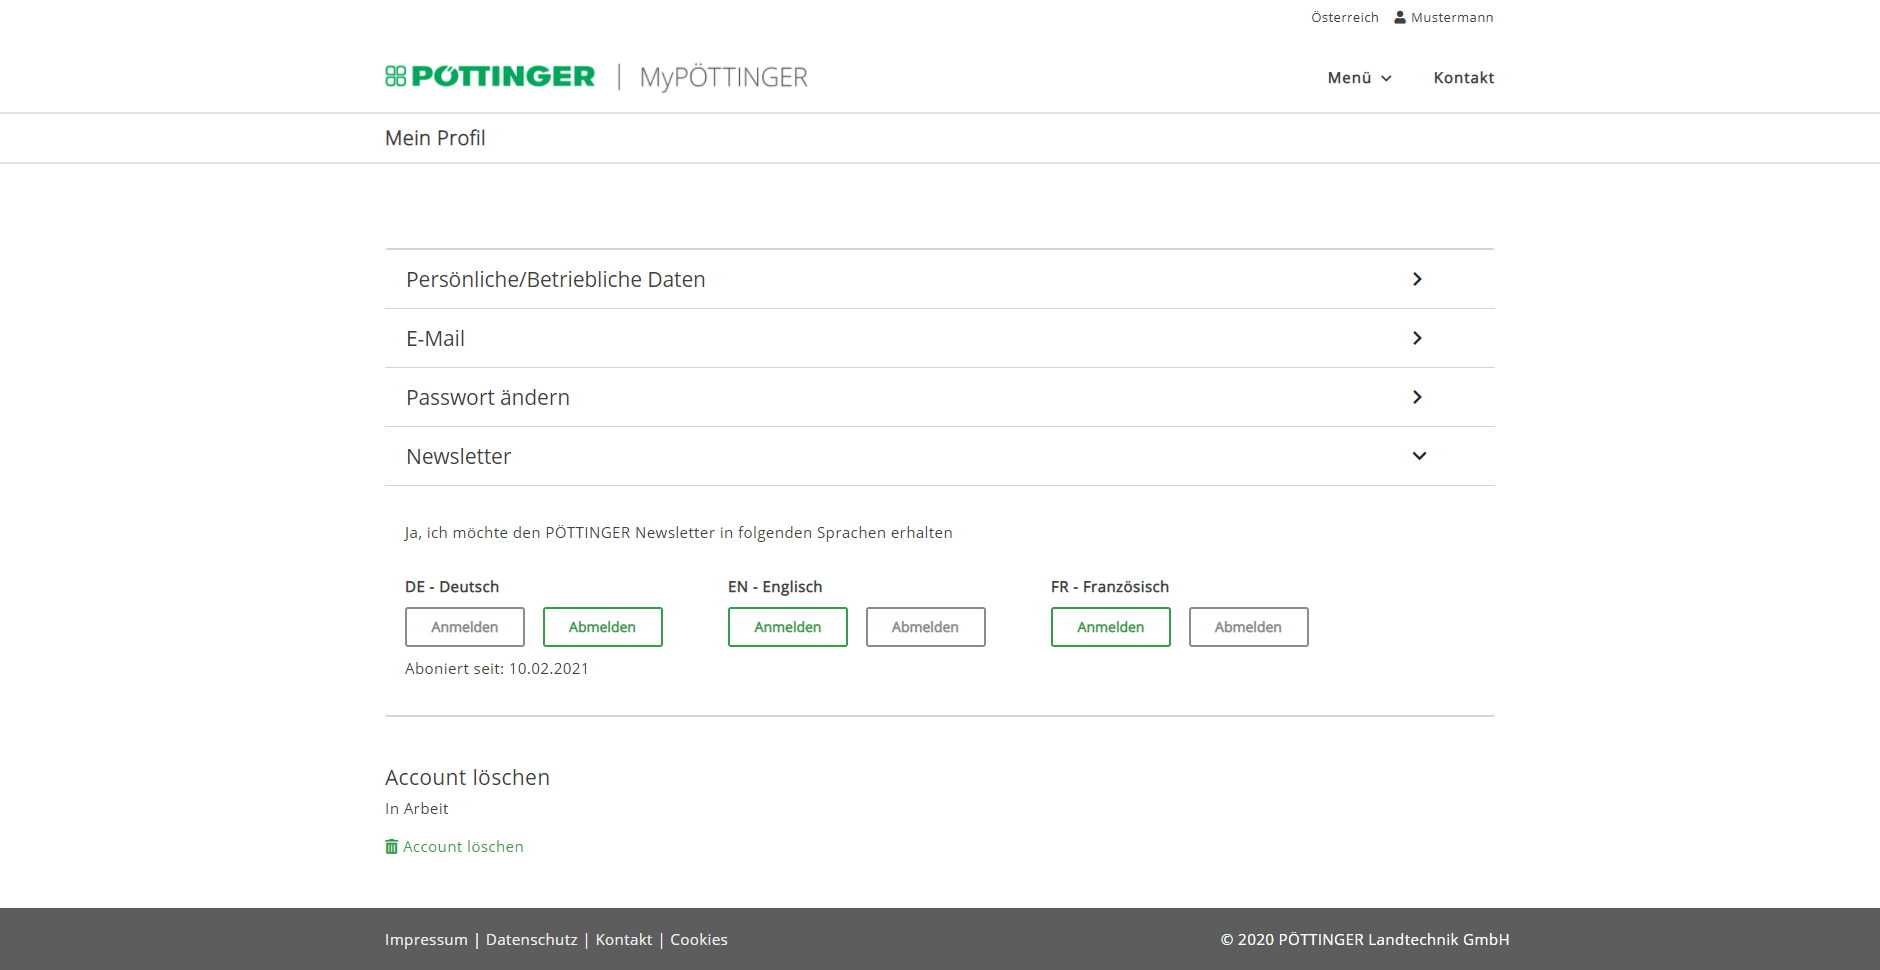
\includegraphics[width=1\textwidth, frame]{./grafiken/erm_profil_newsletter.png}
	}
	\vskip0pt
	\caption{Newsletter} \label{fig:newsletter}
\end{figure}

\section{Produktpalette}

Mit der Produktpalette erhält man eine Vielzahl an Informationen zu den Landmaschinen der Firma Pöttinger. Um die gewünschte Maschine zu finden, gibt es verschiedene Möglichkeiten. Eine Möglichkeit ist, die Maschine in der Produktpalette zu suchen. Dafür klickt man auf "Suche in der Produktpalette" und danach öffnet sich eine Baumstruktur, in der man von oben nach unten in den Kategorien suchen kann. Am Beginn stehen Grünland und Ackerbau zur Auswahl. Öffnet man Grünland, erscheinen die Unterkategorien dieser Art. Es gibt bis zu fünf Ebenen, bis man zu den einzelnen Maschinen gelangt. Diese Suche in der Baumstruktur kann man mit einer Eingabe in der Stichwortsuche über dem Baum noch einschränken. Wenn das eingegebene Stichwort in einer Ebene und darunter nicht vorkommt, ist diese Ebene auch nicht mehr sichtbar. In Abbildung \ref{fig:produktpalette} sieht man die geschlossene Produktpalette. In der Abbildung \ref{fig:produktpaletteOffen} sieht man ein Beispiel für Produktpalette mit geöffneten Unterebenen und die Abbildung \ref{fig:produktpaletteMitStichwort} zeigt den Unterschied, wenn man die offene Produktpalette mit einer Stichworteingabe verbindet.

\begin{figure}[H]
	\centerline{
		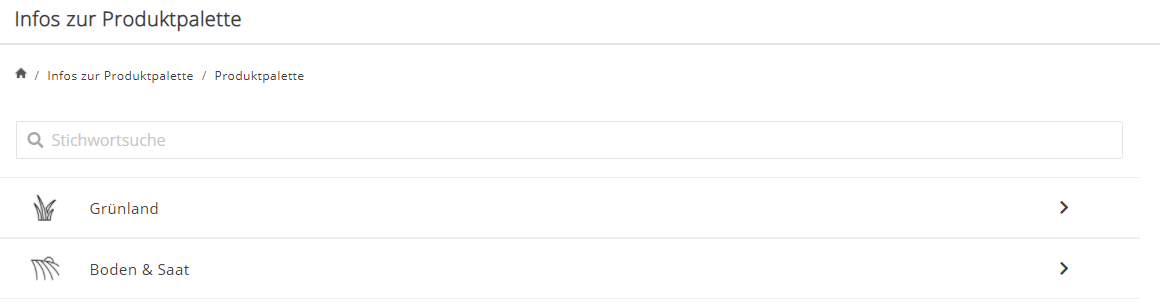
\includegraphics[width=1\textwidth, frame]{./grafiken/erm_produktpalette_neu_.png}
	}
	\vskip0pt
	\caption{Produktpalette} \label{fig:produktpalette}
\end{figure}

\begin{figure}[H]
	\centerline{
		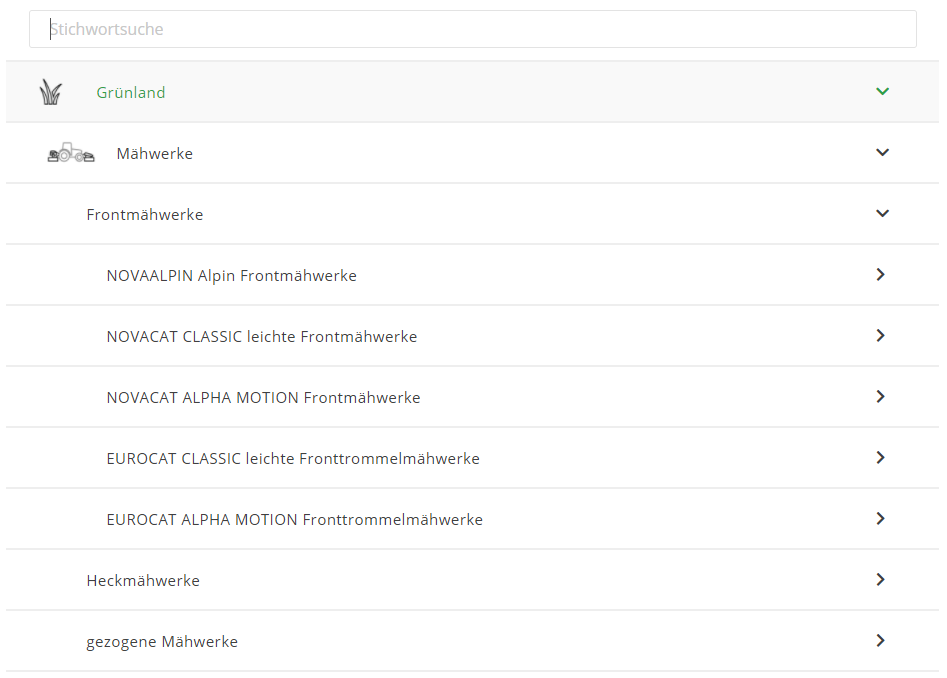
\includegraphics[width=1\textwidth, frame]{./grafiken/erm_produktpalette_offen.png}
	}
	\vskip0pt
	\caption{Offene Produktpalette} \label{fig:produktpaletteOffen}
\end{figure}

\begin{figure}[H]
	\centerline{
		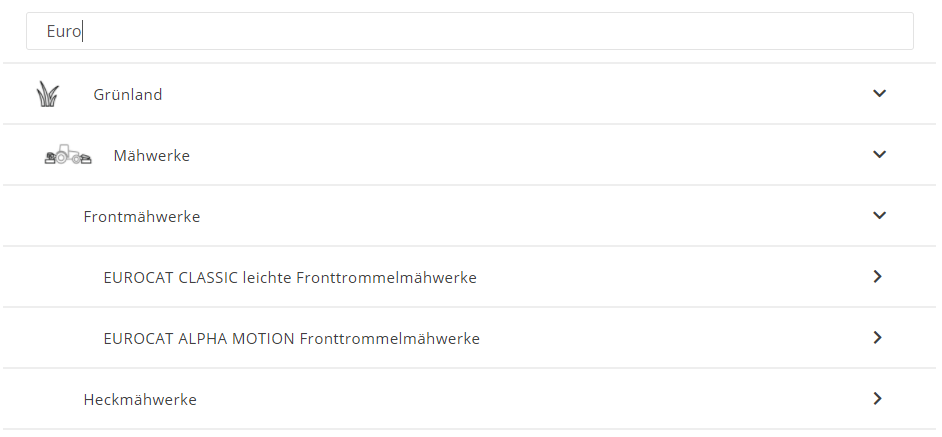
\includegraphics[width=1\textwidth, frame]{./grafiken/erm_produktpalette_offen_stichwort.PNG}
	}
	\vskip0pt
	\caption{Offene Produktpalette mit Stichwortsuche} \label{fig:produktpaletteMitStichwort}
\end{figure}

Eine andere Möglichkeit ist außerdem die Suche mit einer gültigen Maschinennummer. Wird diese Nummer eingegeben, gelangt man direkt zur Produktübersicht.

\section{Produktübersicht}

Wurde eine Maschine in der Produktpalette, direkt mit der Maschinennummer oder eine im Maschinenpark gespeicherte Maschine gesucht, gelangt man auf die Produktübersicht, die man in Abbildung \ref{fig:produktübersicht} erkennen kann. Hier findet man jegliche nützliche Informationen über die ausgewählte Maschine. Die angezeigten Informationen variieren je nach Maschine und Verfügbarkeit.

\begin{figure}[H]
	\centerline{
		\includegraphics[width=1\textwidth, frame]{./grafiken/erm_produktübersicht.png}
	}
	\vskip0pt
	\caption{Produktübersicht} \label{fig:produktübersicht}
\end{figure}

\subsection{Highlights}

Bei den Highlights des Produktes werden wissenswerte Informationen in Form eines Bildes mit einer Überschrift aufgelistet. Das zeigt die Abbildung \ref{fig:highlight}.
\begin{figure}[H]
	\centerline{
		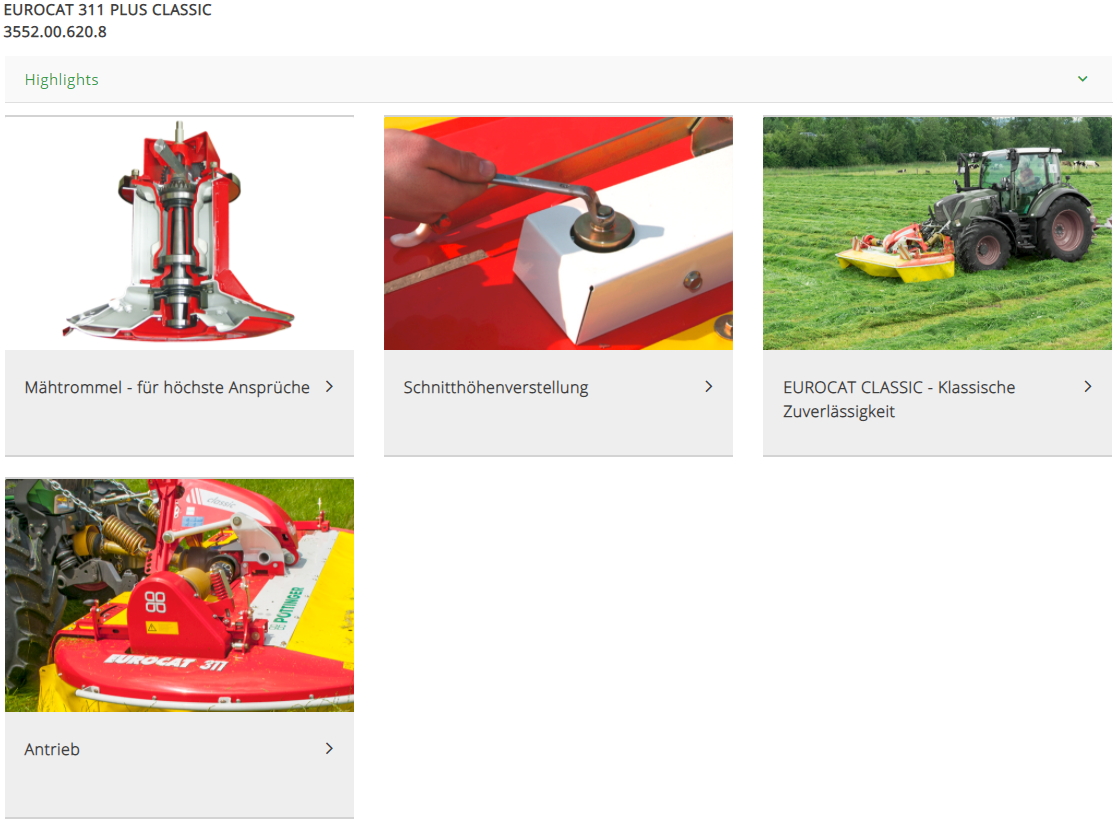
\includegraphics[width=1\textwidth, frame]{./grafiken/erm_detailansicht_highlights.PNG}
	}
	\vskip0pt
	\caption{Highlights} \label{fig:highlight}
\end{figure}
 Wird nun ein Highlight ausgewählt, gelangt man zu einer genaueren Beschreibung der jeweiligen Besonderheit. Einen dieser Artikel sieht man in Abbildung \ref{fig:highlightbeschreibung}.
\begin{figure}[H]
	\centerline{
		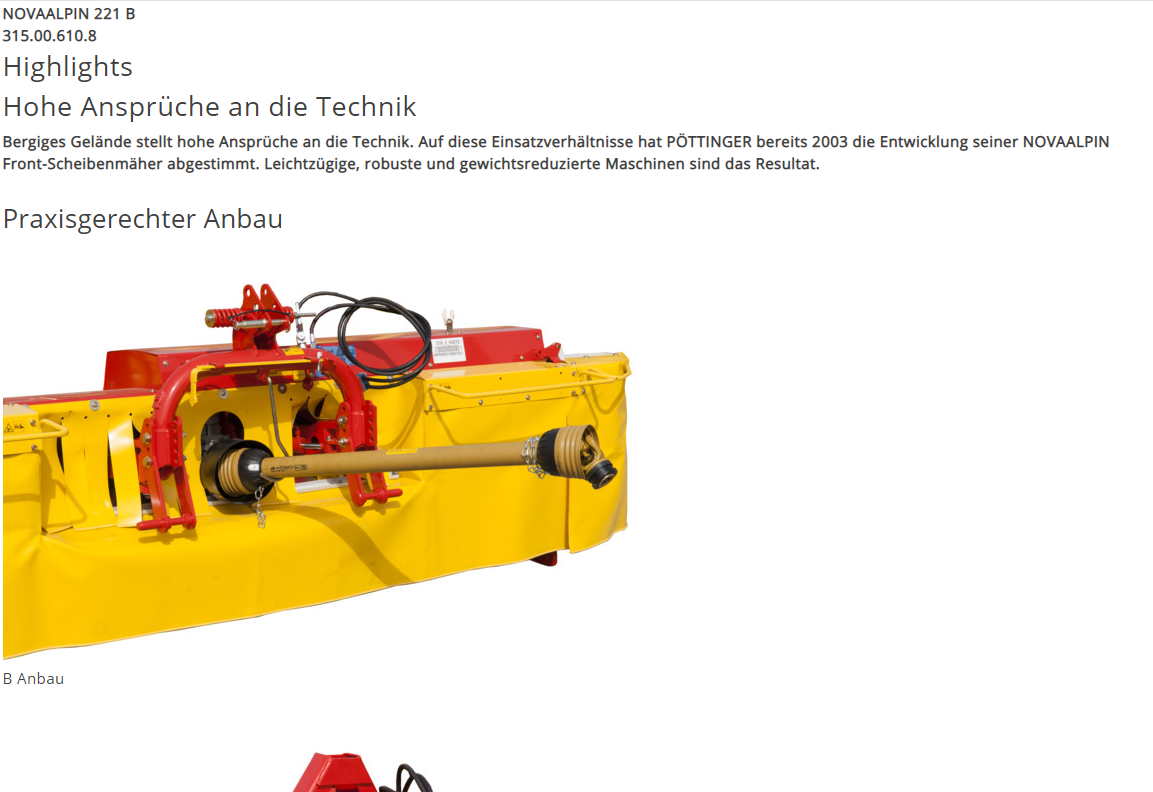
\includegraphics[width=1\textwidth, frame]{./grafiken/erm_detailansicht_highlights_beschreibung.PNG}
	}
	\vskip0pt
	\caption{Highlight-Beschreibung} \label{fig:highlightbeschreibung}
\end{figure}

\subsection{Ausstattung}

Bei der Ausstattung findet man die verbauten Teile. Wie in Abbildung \ref{fig:ausstattung} sieht man diese Teile mit der jeweiligen Materialnummer und einer Bezeichnung aufgelistet. Darunter sind noch optionale Ausrüstungen aufgelistet, die mit dieser Maschine kompatibel sind.

\begin{figure}[H]
	\centerline{
		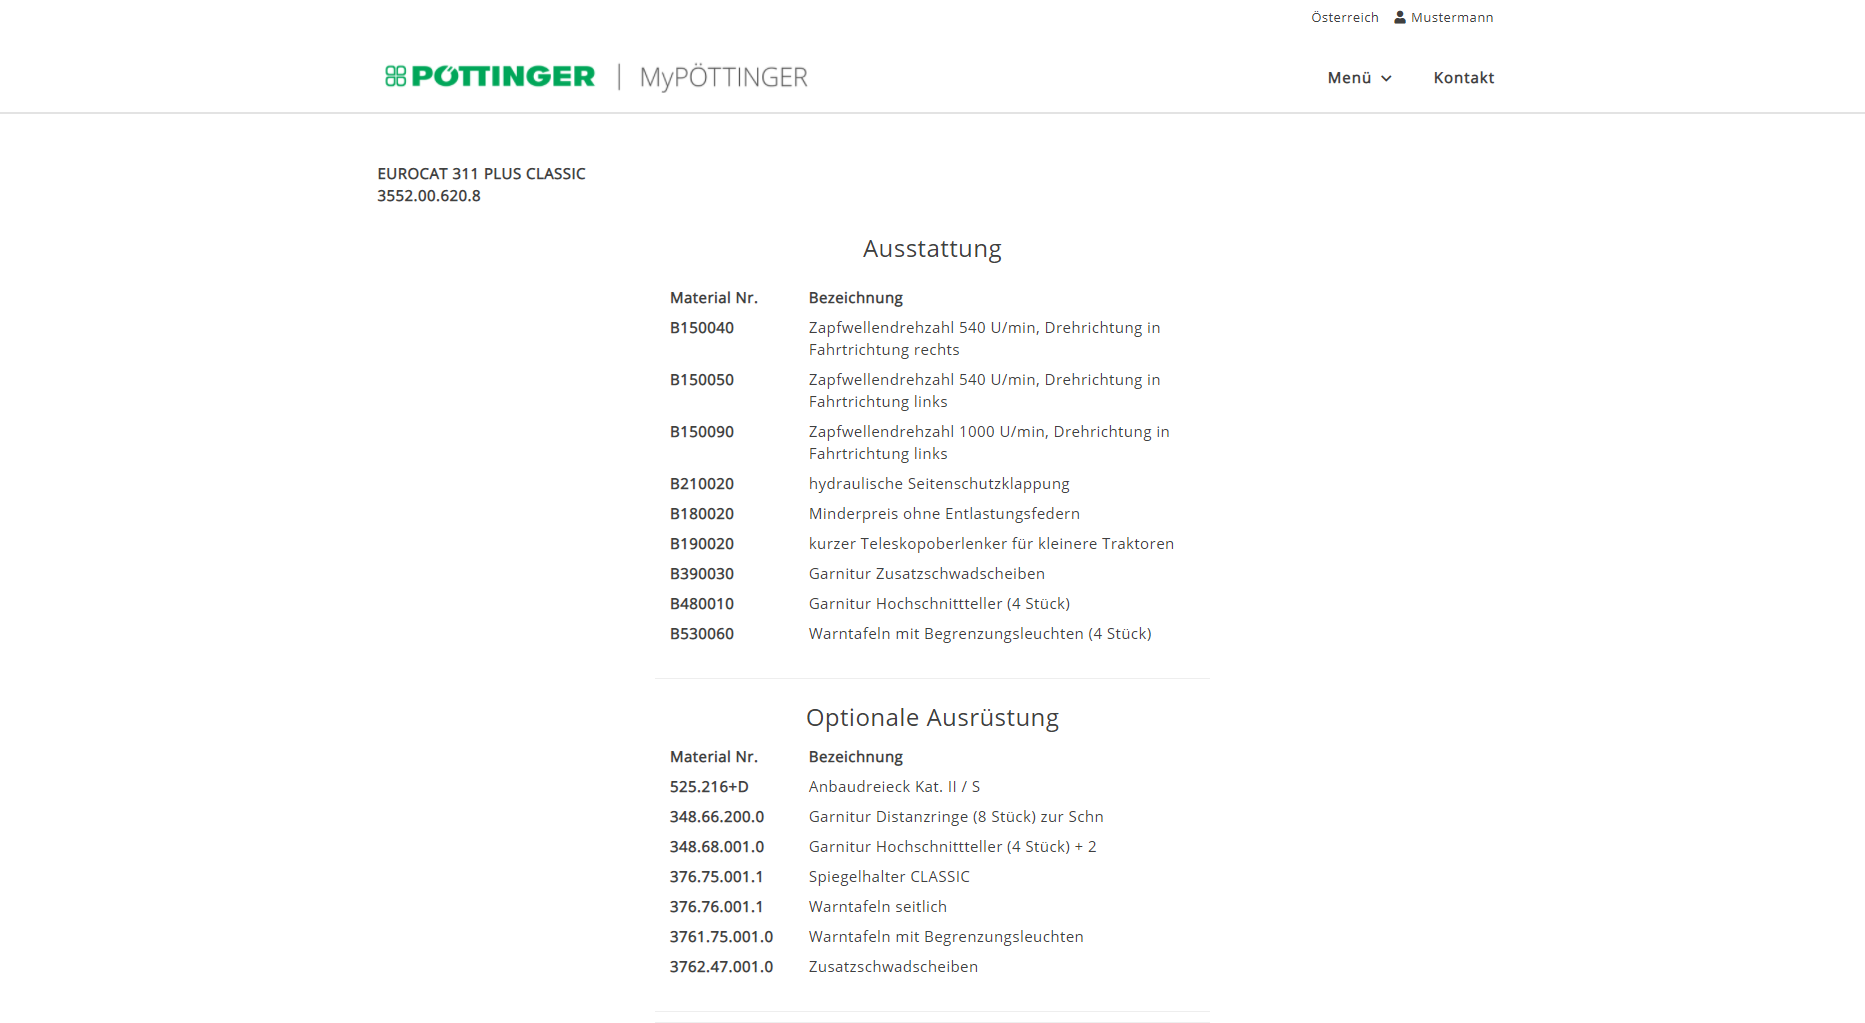
\includegraphics[width=1\textwidth, frame]{./grafiken/erm_detailansicht_ausstattung.PNG}
	}
	\vskip0pt
	\caption{Ausstattung} \label{fig:ausstattung}
\end{figure}

\subsection{Technische Daten}

Bei den technischen Daten in Abbildung \ref{fig:technischeDaten} findet man nützliche Informationen wie Anbau, Gewicht, Arbeitsbreite, Transportbreite, Kraftbedarf und vieles mehr.

\begin{figure}[H]
	\centerline{
		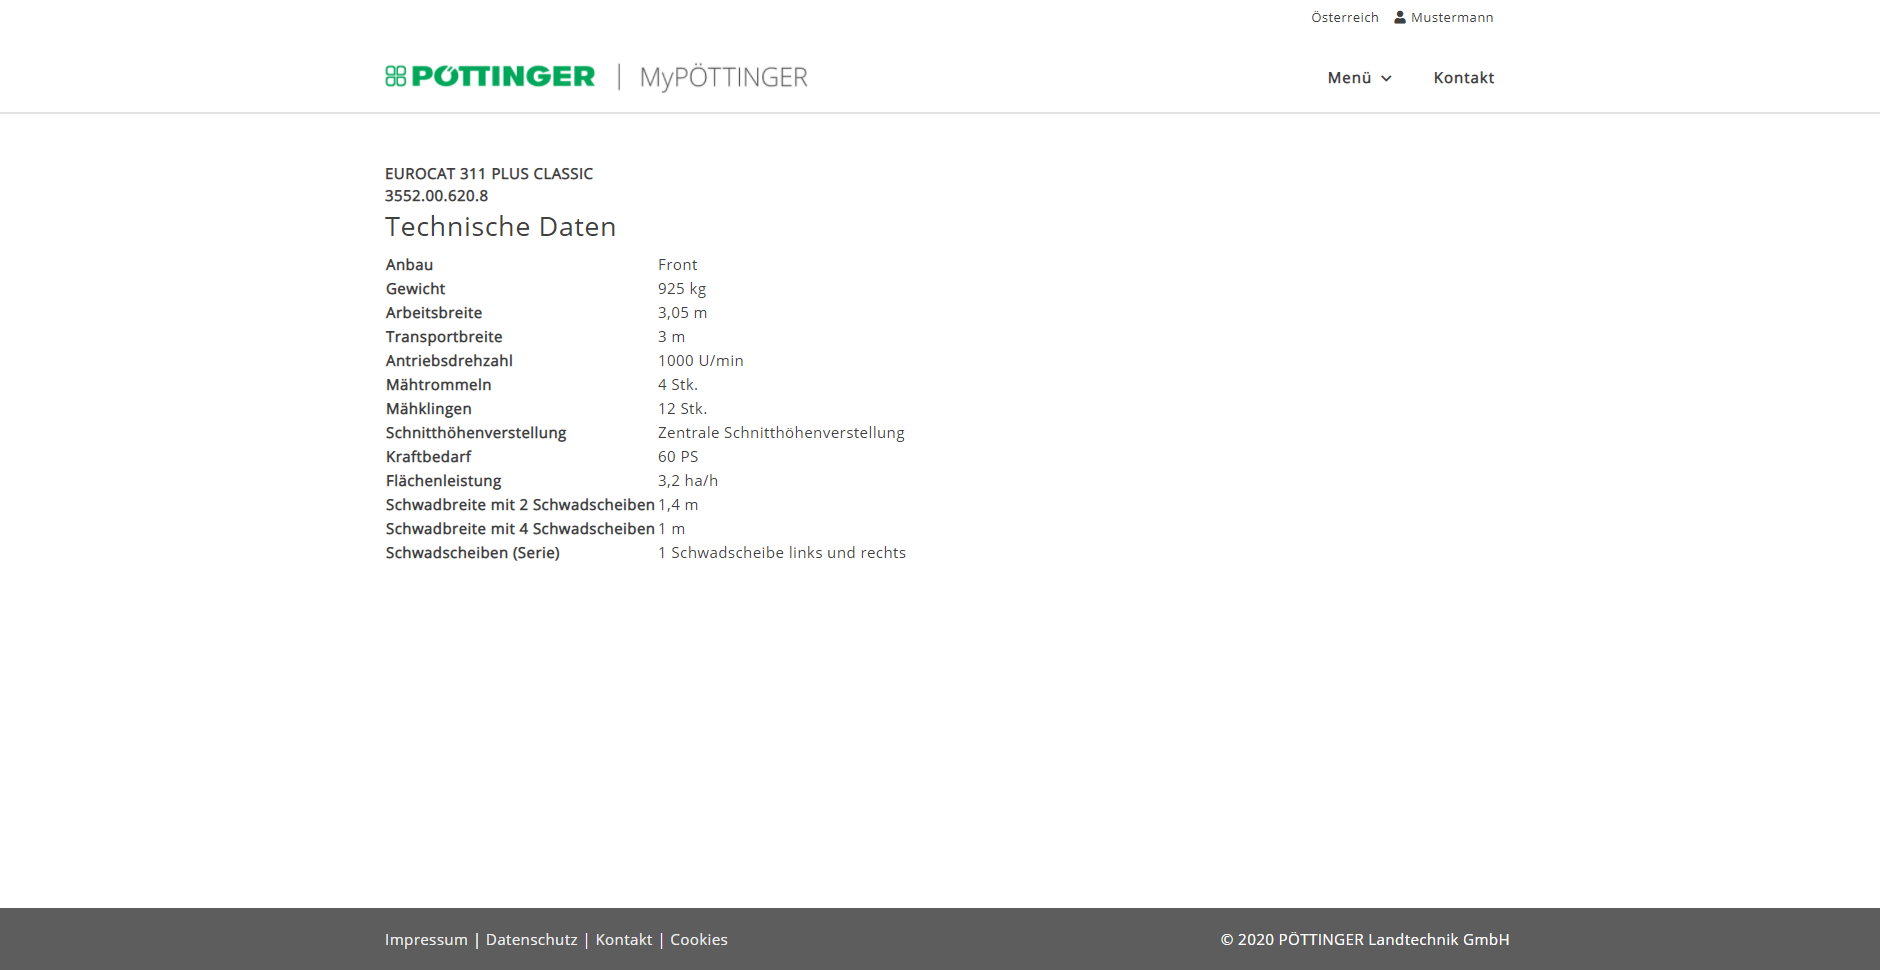
\includegraphics[width=1\textwidth, frame]{./grafiken/erm_detailansicht_technisch.PNG}
	}
	\vskip0pt
	\caption{Ausstattung} \label{fig:technischeDaten}
\end{figure}
\subsection{Videos, Bilder, Prospekte und Betriebsanleitung}
In diesen Kategorien findet man Videos, Bilder, Prospekte und eine Betriebsanleitung für die Maschine. Diese Videos werden mit YouTube abgespielt. Die Prospekte und die Betriebsanleitung sind zum Download verfügbar. Da nicht von jeder Maschine Bilder oder Videos vorhanden sind, gibt es dieses Feld auch nicht bei jeder Detailansicht.
\section{Maschinenpark}

In Abbildung \ref{fig:maschinenpark} sieht man den Maschinenpark, in dem eine Auflistung aller gespeicherten Maschinen des Benutzers gezeigt wird. Somit hat der Nutzer einen schnellen Zugriff auf nützliche Tipps zur der gespeicherten Maschine, sowie zu Bedienungsanleitungen, Ersatzteillisten, Wartungsinformationen und allen technischen Details und Unterlagen.

\begin{figure}[H]
	\centerline{
		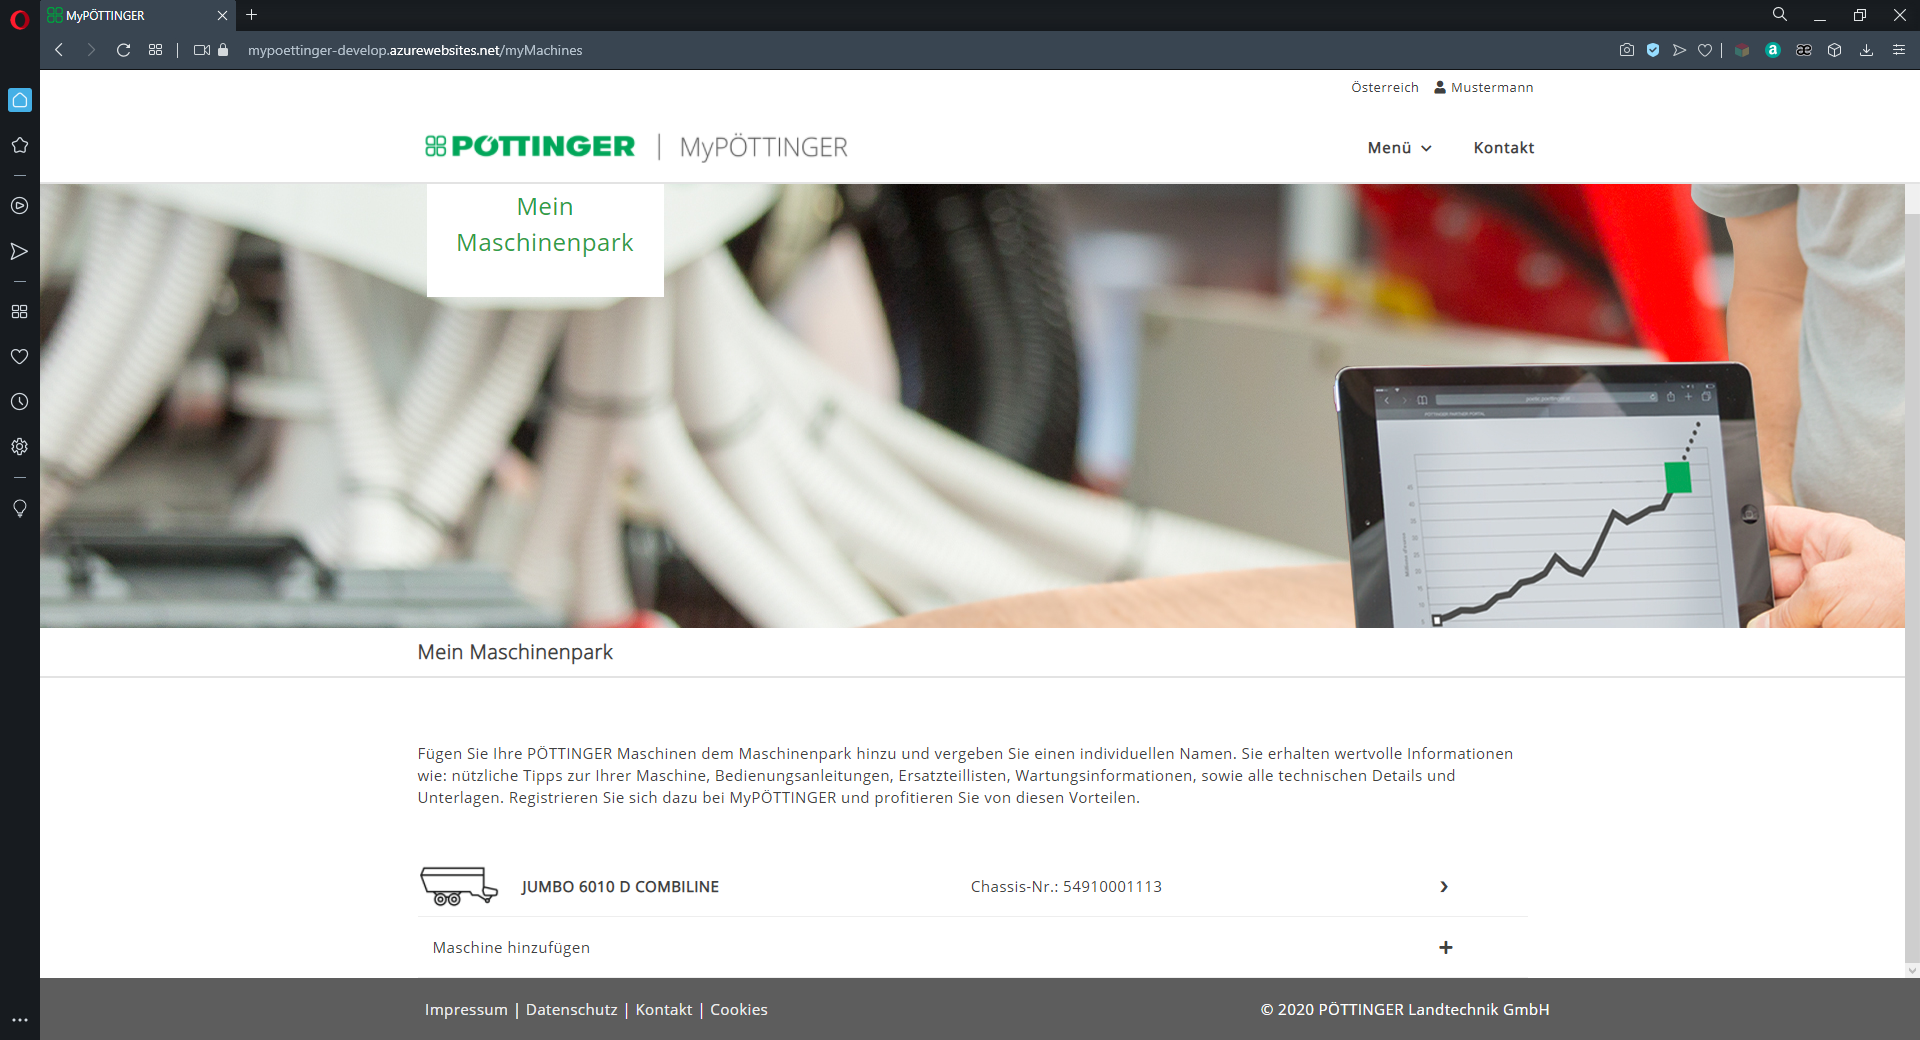
\includegraphics[width=1\textwidth, frame]{./grafiken/erm_maschinenpark.png}
	}
	\vskip0pt
	\caption{Maschinenpark} \label{fig:maschinenpark}
\end{figure}

Navigiert man über den Maschinenpark zu der gespeicherten Maschine, ändert sich die Detailansicht, wie in Abbildung \ref{fig:savedMaschine} ersichtlich, etwas. Hinzu kommt ein Bild der Maschine und es wird die Möglichkeit geboten, dieser Maschine einen individuellen Namen zu geben.

\begin{figure}[H]
	\centerline{
		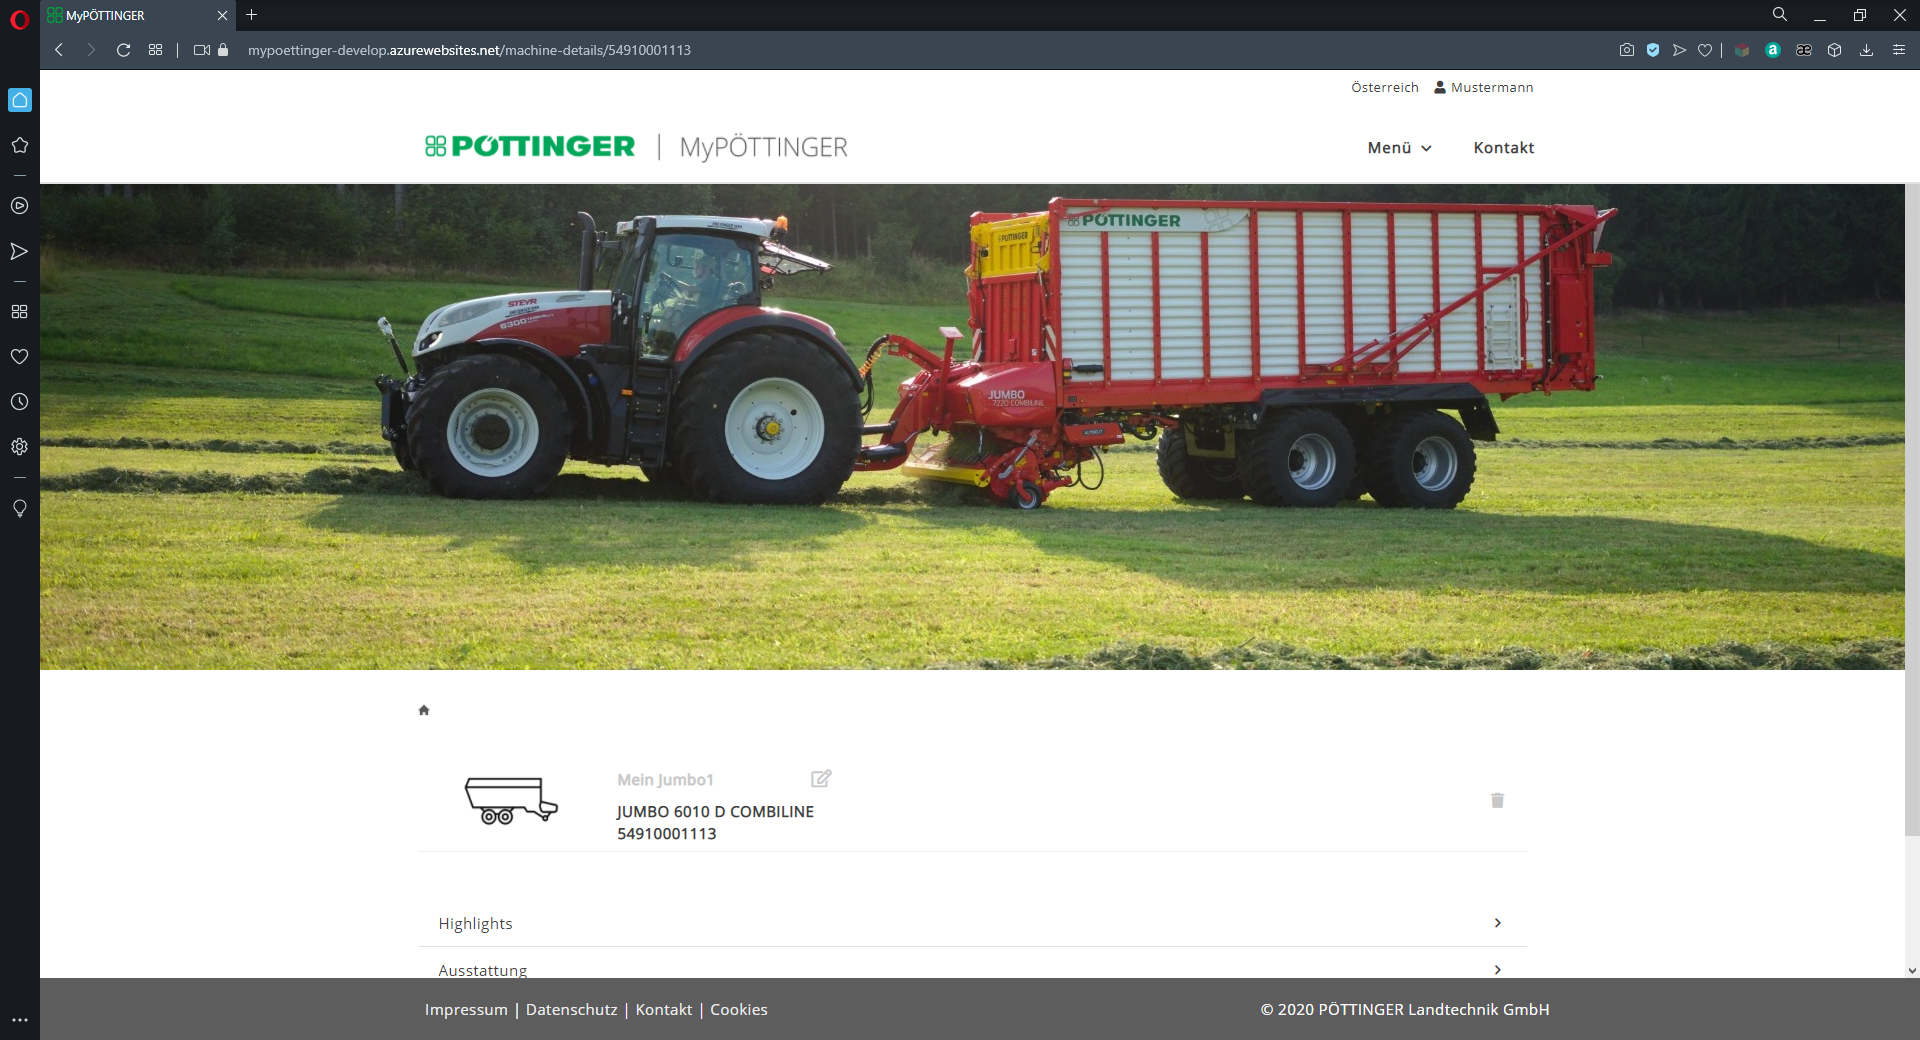
\includegraphics[width=1\textwidth, frame]{./grafiken/erm_detailansicht_saved_machine.png}
	}
	\vskip0pt
	\caption{Detailansicht der gespeicherten Maschine} \label{fig:savedMaschine}
\end{figure}

Wenn die Maschine einen individuellen Namen erhalten hat, wird dieser Name auch im eigenen Maschinenpark wie in Abbildung \ref{fig:benannteMaschine} angezeigt:
 
\begin{figure}[H]
	\centerline{
		
\includegraphics[width=1\textwidth, frame]{./grafiken/erm_maschinenpark_benannteMaschine.png}
	}
	\vskip0pt
	\caption{Benannte Maschine} \label{fig:benannteMaschine}
\end{figure}
	
	%%%%%%%%%%%%%%%%%%%%%%%%%%%%%%%%%%%%%%%%%
	%%%   DANKSAGUNG   %%%%%%%%%%%%%%%%%%%%%%
	%%%%%%%%%%%%%%%%%%%%%%%%%%%%%%%%%%%%%%%%%
	
	\chapter{Danksagung}
Einen Großen Dank wollen wir an unsere Eltern aussprechen, die es uns ermöglicht haben, die HTBLA Grieskirchen zu besuchen.\\
Wir möchten uns auch sehr herzlich beim Auftraggeber unserer Diplomarbeit, dem Unternehmen \ThPartnerName \,, für das Vertrauen und die Bereitstellung der Diplomarbeit bedanken.\\
Ebenfalls bedanken wir uns bei allen Professorinnen und Professoren, die uns bei technischen und organisatorischen Fragen Ihre Hilfen angeboten haben. Besonders möchten wir unseren Dank gegenüber unserem Diplomarbeitsbetreuer \ThSupervisorName \, aussprechen.
	
	%%%%%%%%%%%%%%%%%%%%%%%%%%%%%%%%%%%%%%%%%
	%%%   BIBLIOGRAPHY   %%%%%%%%%%%%%%%%%%%%
	%%%%%%%%%%%%%%%%%%%%%%%%%%%%%%%%%%%%%%%%%
	
	\pagestyle{empty}
	\rfoot{}
	\lfoot{}
	\renewcommand{\footrulewidth}{0pt}
	\printbibliography[title={\hspace{\fill}Literaturverzeichnis}]
	\thispagestyle{empty}
	
	%%%%%%%%%%%%%%%%%%%%%%%%%%%%%%%%%%%%%%%%%
	%%%   BEGLEITPROTOKOLL   %%%%%%%%%%%%%%%%
	%%%%%%%%%%%%%%%%%%%%%%%%%%%%%%%%%%%%%%%%%
	
	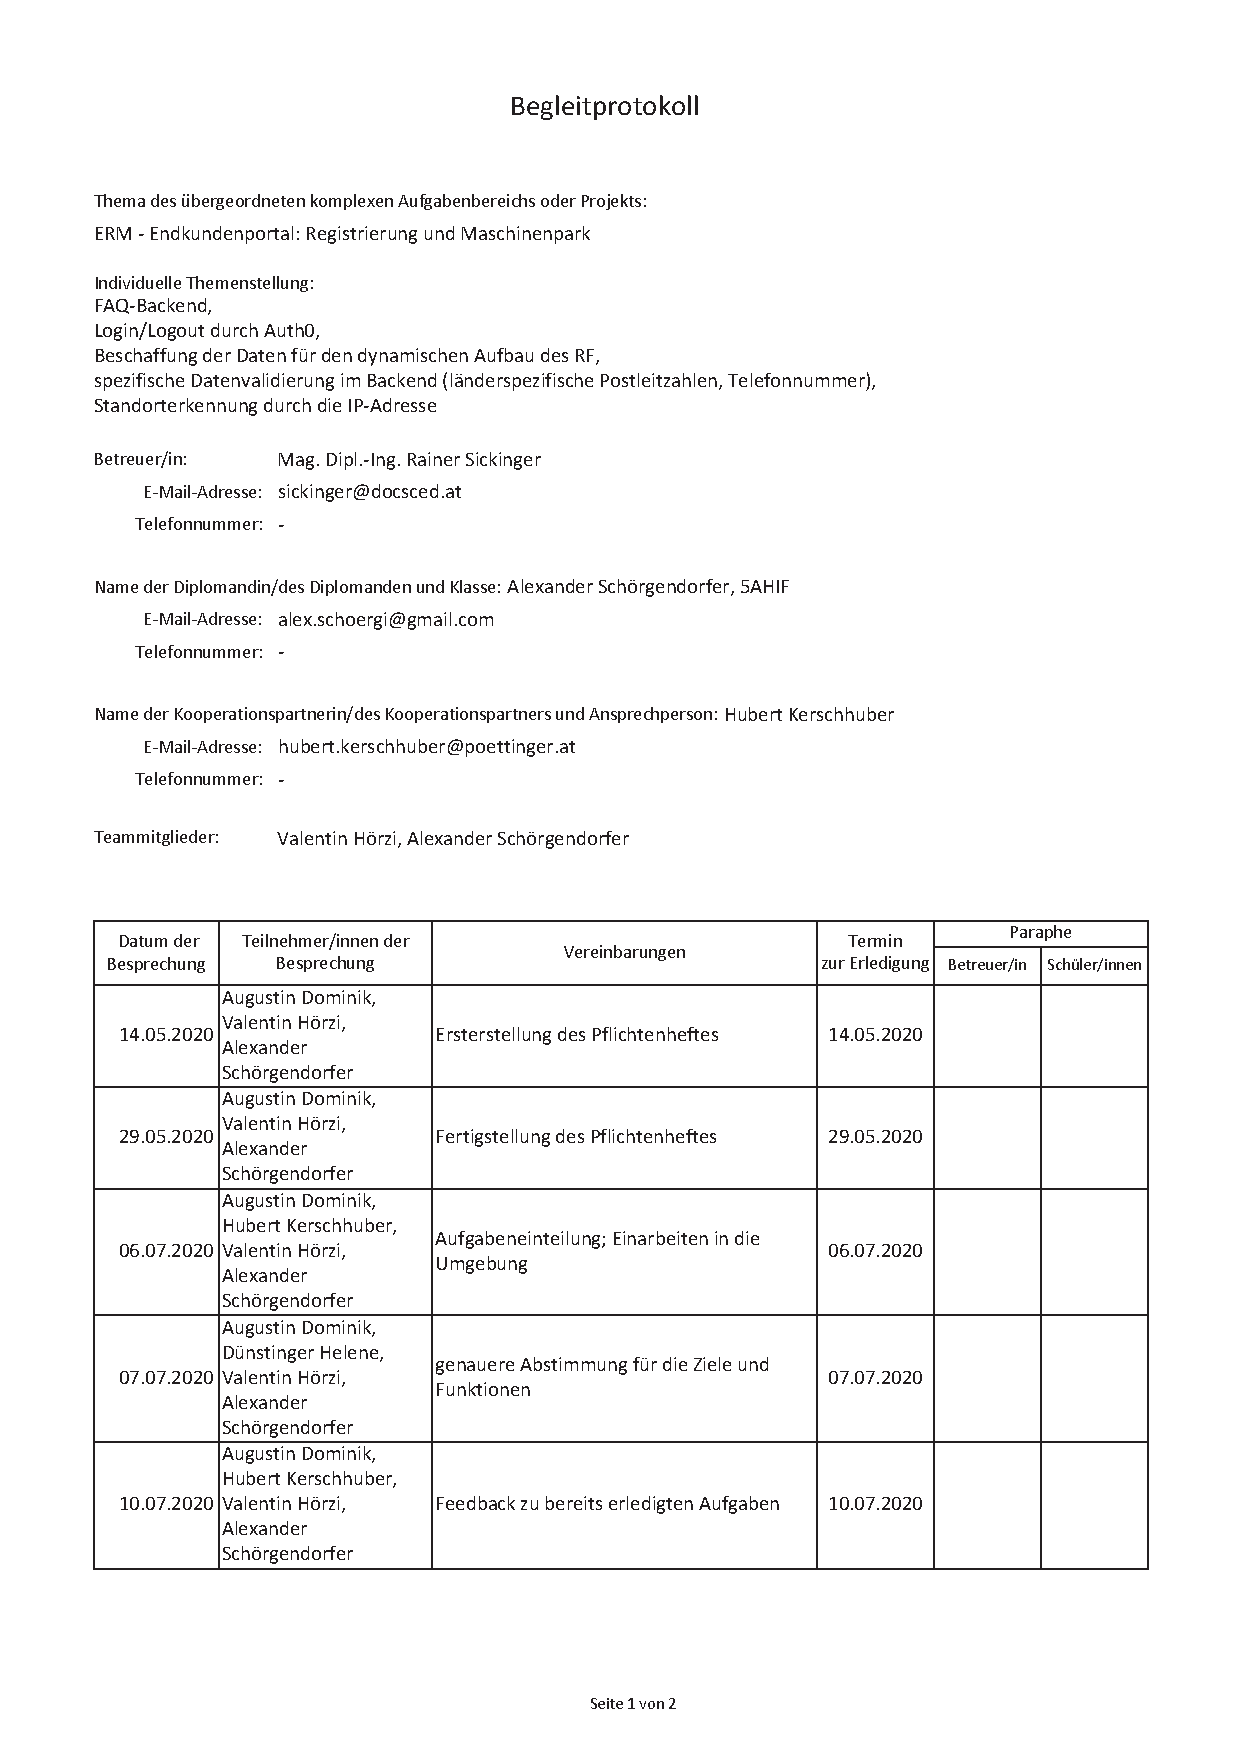
\includepdf[pages={1-2}]{./kapitel/anhang/Begleitprotokoll_schoergendorfer_to_show.PDF}
	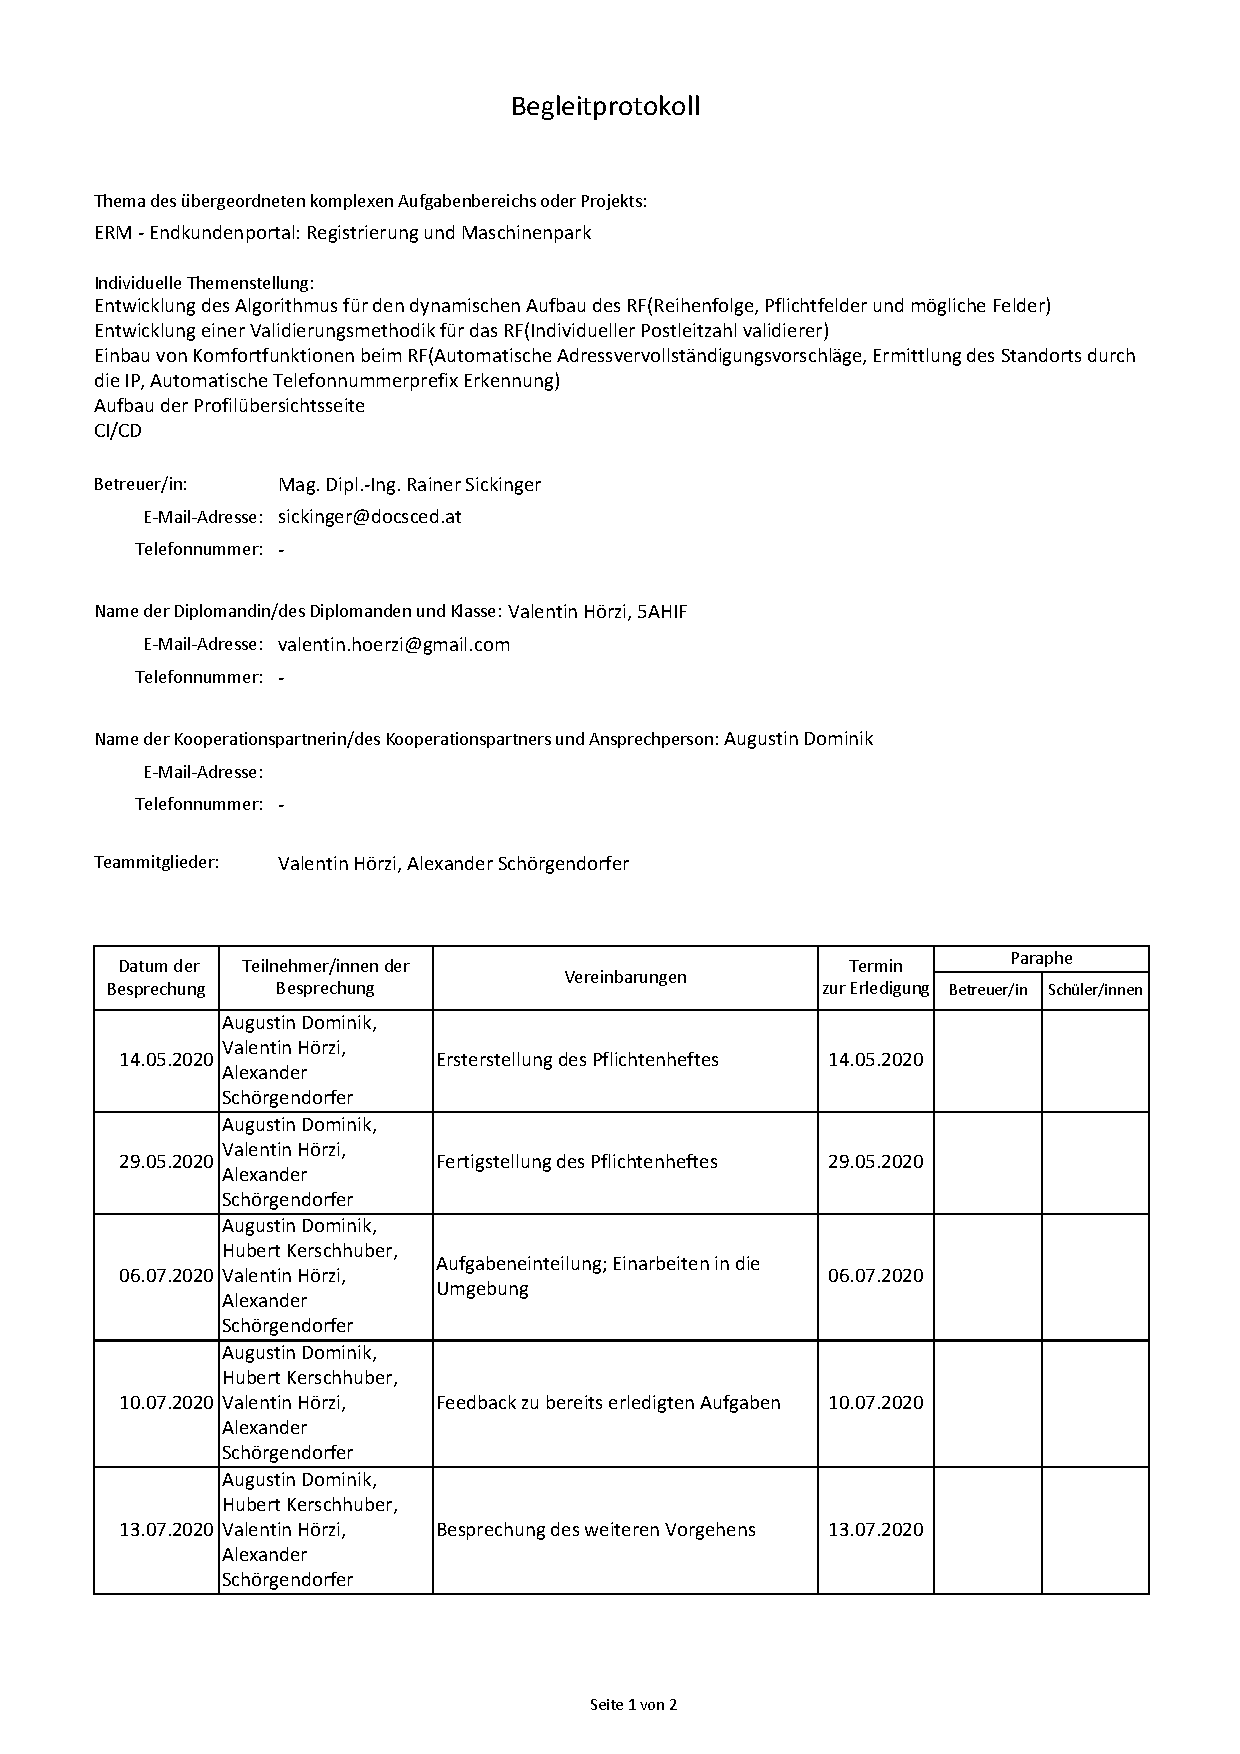
\includepdf[pages={1-2}]{./kapitel/anhang/Begleitprotokoll_hoerzi_to_show.PDF}
	
	%%%%%%%%%%%%%%%%%%%%%%%%%%%%%%%%%%%%%%%%%
	%%%   LIST OF FIGURES   %%%%%%%%%%%%%%%%%
	%%%%%%%%%%%%%%%%%%%%%%%%%%%%%%%%%%%%%%%%%
	
	\rfoot{}
	\lfoot{}
	%%%%%%%%% untenstehende Gruppe ist dafür, dass keine Pagenumber beim Abbildungsverzeichnis ist
	\clearpage
	\begingroup 
	\makeatletter
	\let\ps@plain\ps@empty
	\makeatother
	
	\pagestyle{empty}
	\renewcommand{\listfigurename}{Abbildungsverzeichnis}
	\listoffigures
	\cleardoublepage
	\endgroup

	\pagebreak
	
	%%%%%%%%%%%%%%%%%%%%%%%%%%%%%%%%%%%%%%%%%
	%%%   LIST OF LISTINGS  %%%%%%%%%%%%%%%%%
	%%%%%%%%%%%%%%%%%%%%%%%%%%%%%%%%%%%%%%%%%
	
	\renewcommand{\lstlistlistingname}{Listingverzeichnis}
	\lstlistoflistings	
	\thispagestyle{empty}
	\pagebreak
	
	%%%%%%%%%%%%%%%%%%%%%%%%%%%%%%%%%%%%%%%%%
	%%%   LIST OF Tables  %%%%%%%%%%%%%%%%%%%
	%%%%%%%%%%%%%%%%%%%%%%%%%%%%%%%%%%%%%%%%%
	
	\renewcommand{\listtablename}{Tabellenverzeichnis}
	\listoftables	
	\thispagestyle{empty}
	\begin{table}[H]
		\centering
		{\rowcolors{2}{gray!20}{gray!10}
			\setlength{\arrayrulewidth}{1pt}
			\begin{tabular}[h]{|l|p{8cm}|p{2.5cm}|p{2.5cm}|}
				\hline
				\rowcolor[gray]{.6}	Abkürzung & Bedeutung \\
				\hline
				JWT & JSON Web Token\\
				\hline
				FAQ & Frequently Asked Questions \\	
				\hline
				DI & Dependency Injection \\
				\hline
				RF & Registrierungsformular \\
				\hline
				DOM & Document Object Model \\
				\hline
				API & Application Programming Interface \\
				\hline
			\end{tabular}
		}
		\caption{Abkürzungen}
	\end{table}
	
	\pagebreak
	
	%%%%%%%%%%%%%%%%%%%%%%%%%%%%%%%%%%%%%%%%%
	%%%   APPENDIX  %%%%%%%%%%%%%%%%%%%%%%%%%
	%%%%%%%%%%%%%%%%%%%%%%%%%%%%%%%%%%%%%%%%%
	
	\Appendix{
		\thispagestyle{empty}
		\begin{figure}[!hb]
			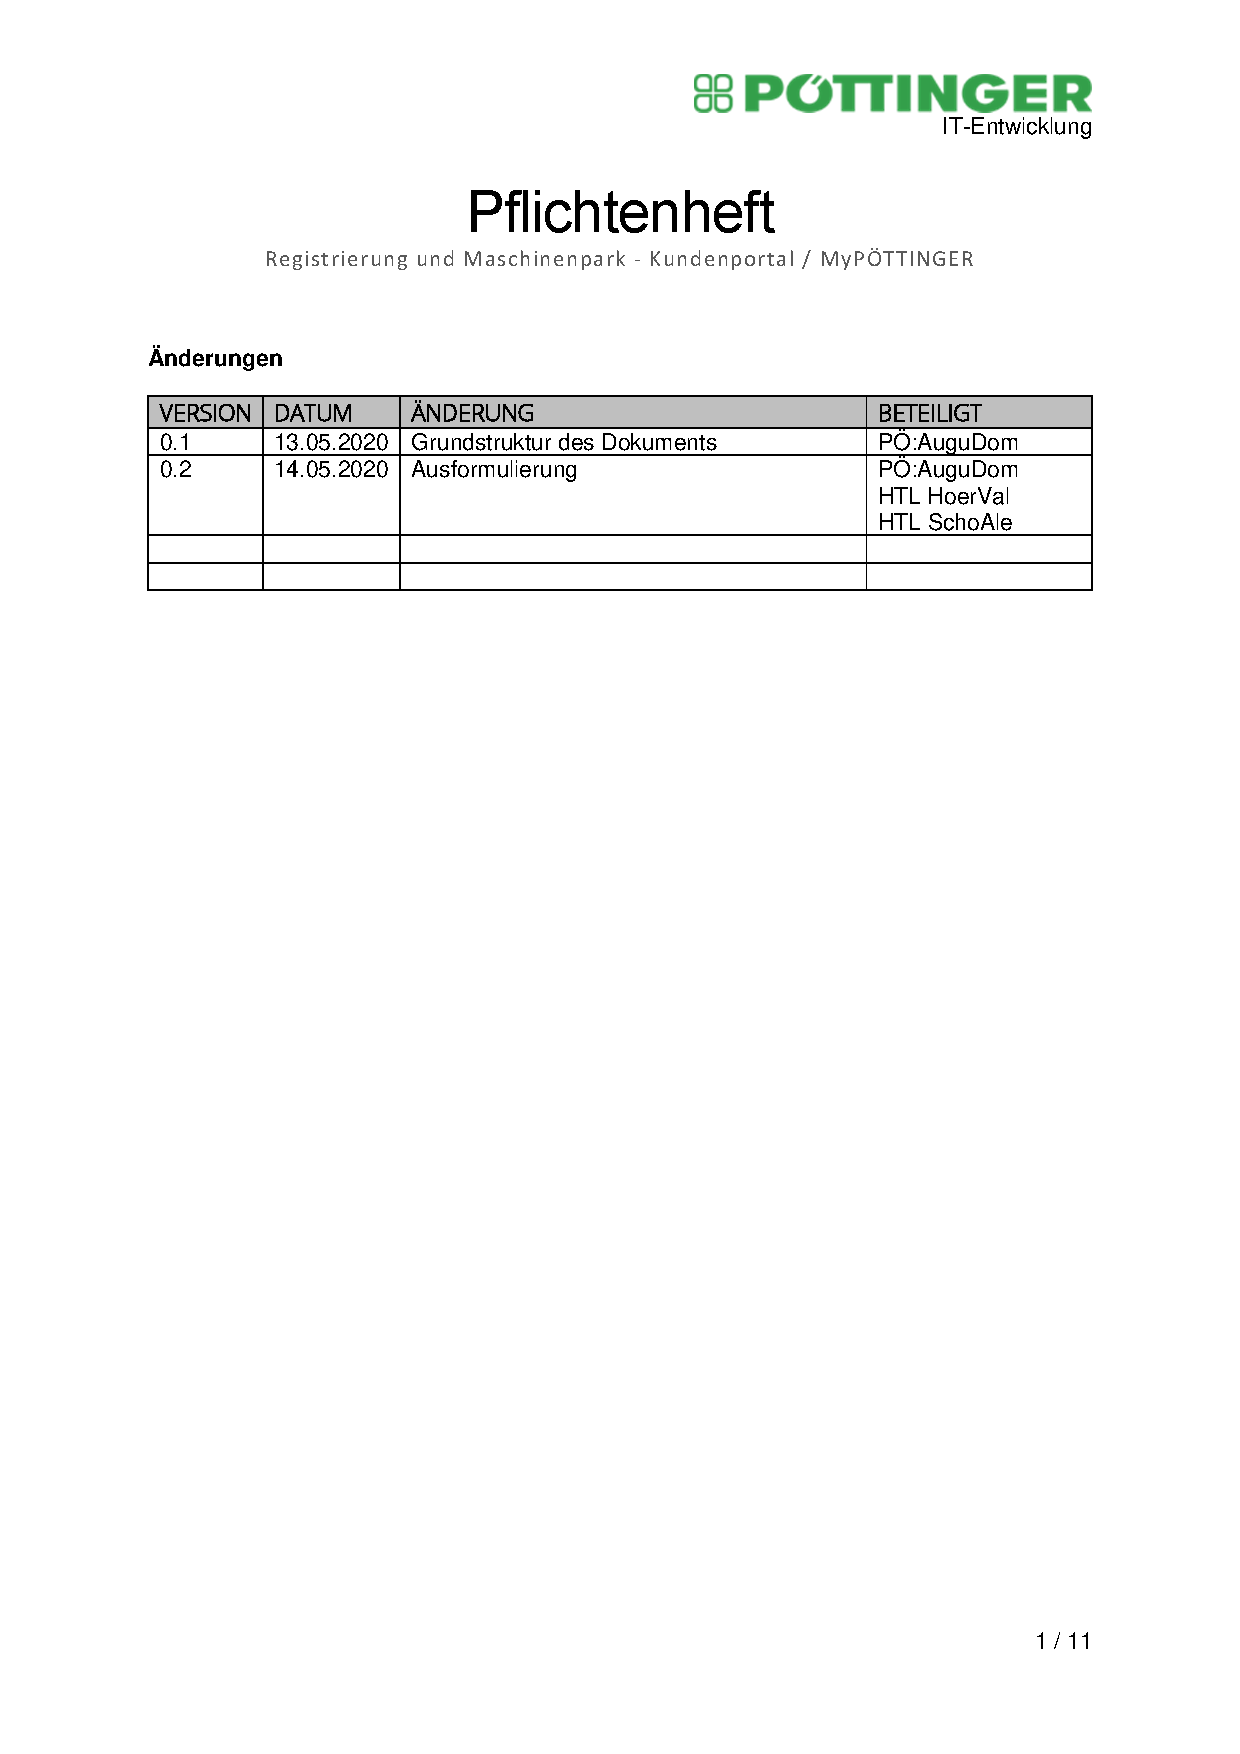
\includepdf[pages={1},  scale=.65, frame=true, pagecommand={}]{./kapitel/anhang/Pflichtenheft_ERM.pdf}
		\end{figure}
		\includepdf[pages={2-11},  scale=.65, frame=true, pagecommand={}]{./kapitel/anhang/Pflichtenheft_ERM.pdf}
	}

\end{document}